\clearpage
\section{IO checks with full simulation MC samples}
\label{app:IO_results}

Additional IO check is performed by repeating the amplitude analysis on 250 sets of toy samples considering the detector response. The signal components are generated by the bootstrap method. The size of each toy is the same as data. Pull distributions for $\alpha_0$ and $\sin\Delta_0$, FFs, decay asymmetry parameters and amplitude magnitudes and phase for the $e^+e^-\to\lcp\lcm$ decay are shown in Figure~\ref{fig:io_wo_bkg_pull_alpha0}-\ref{fig:io_wo_bkg_pull_phase}. The fit results of pull distributions are listed in Table~\ref{tab:fit_io_wo_bkg_pull_polarization}-\ref{tab:fit_io_wo_bkg_pull_gls}. After the same correction mentioned in Sec~\ref{sec:io_check}, the corrected results from two IO checks are consistent within 1$\sigma$ statistical error.
%The output values are consistent with input values within 1$\sigma$ statistical error.

\begin{figure}[h]\centering
    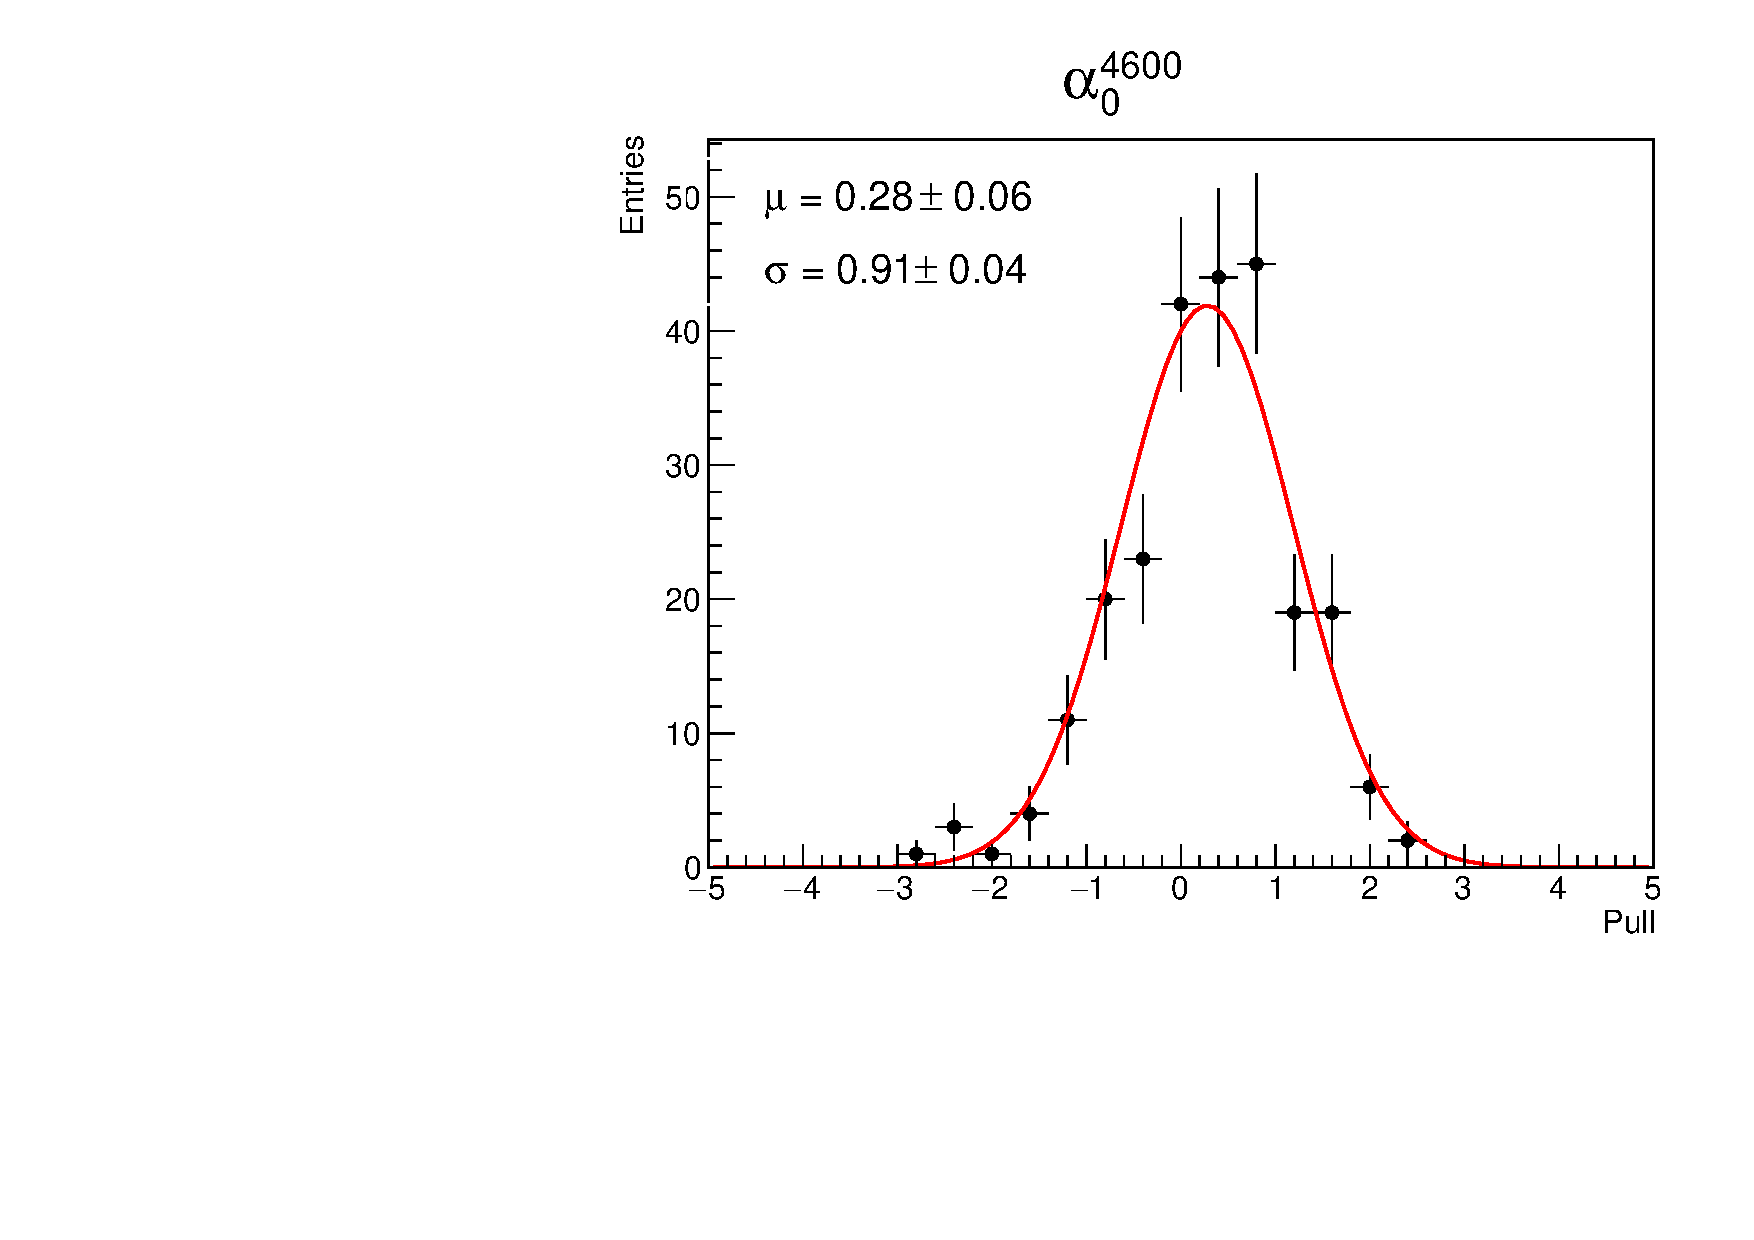
\includegraphics[width=0.24\textwidth]{figure/io_full_sim/polarization/pull_polarization_alpha0_4600.pdf}
    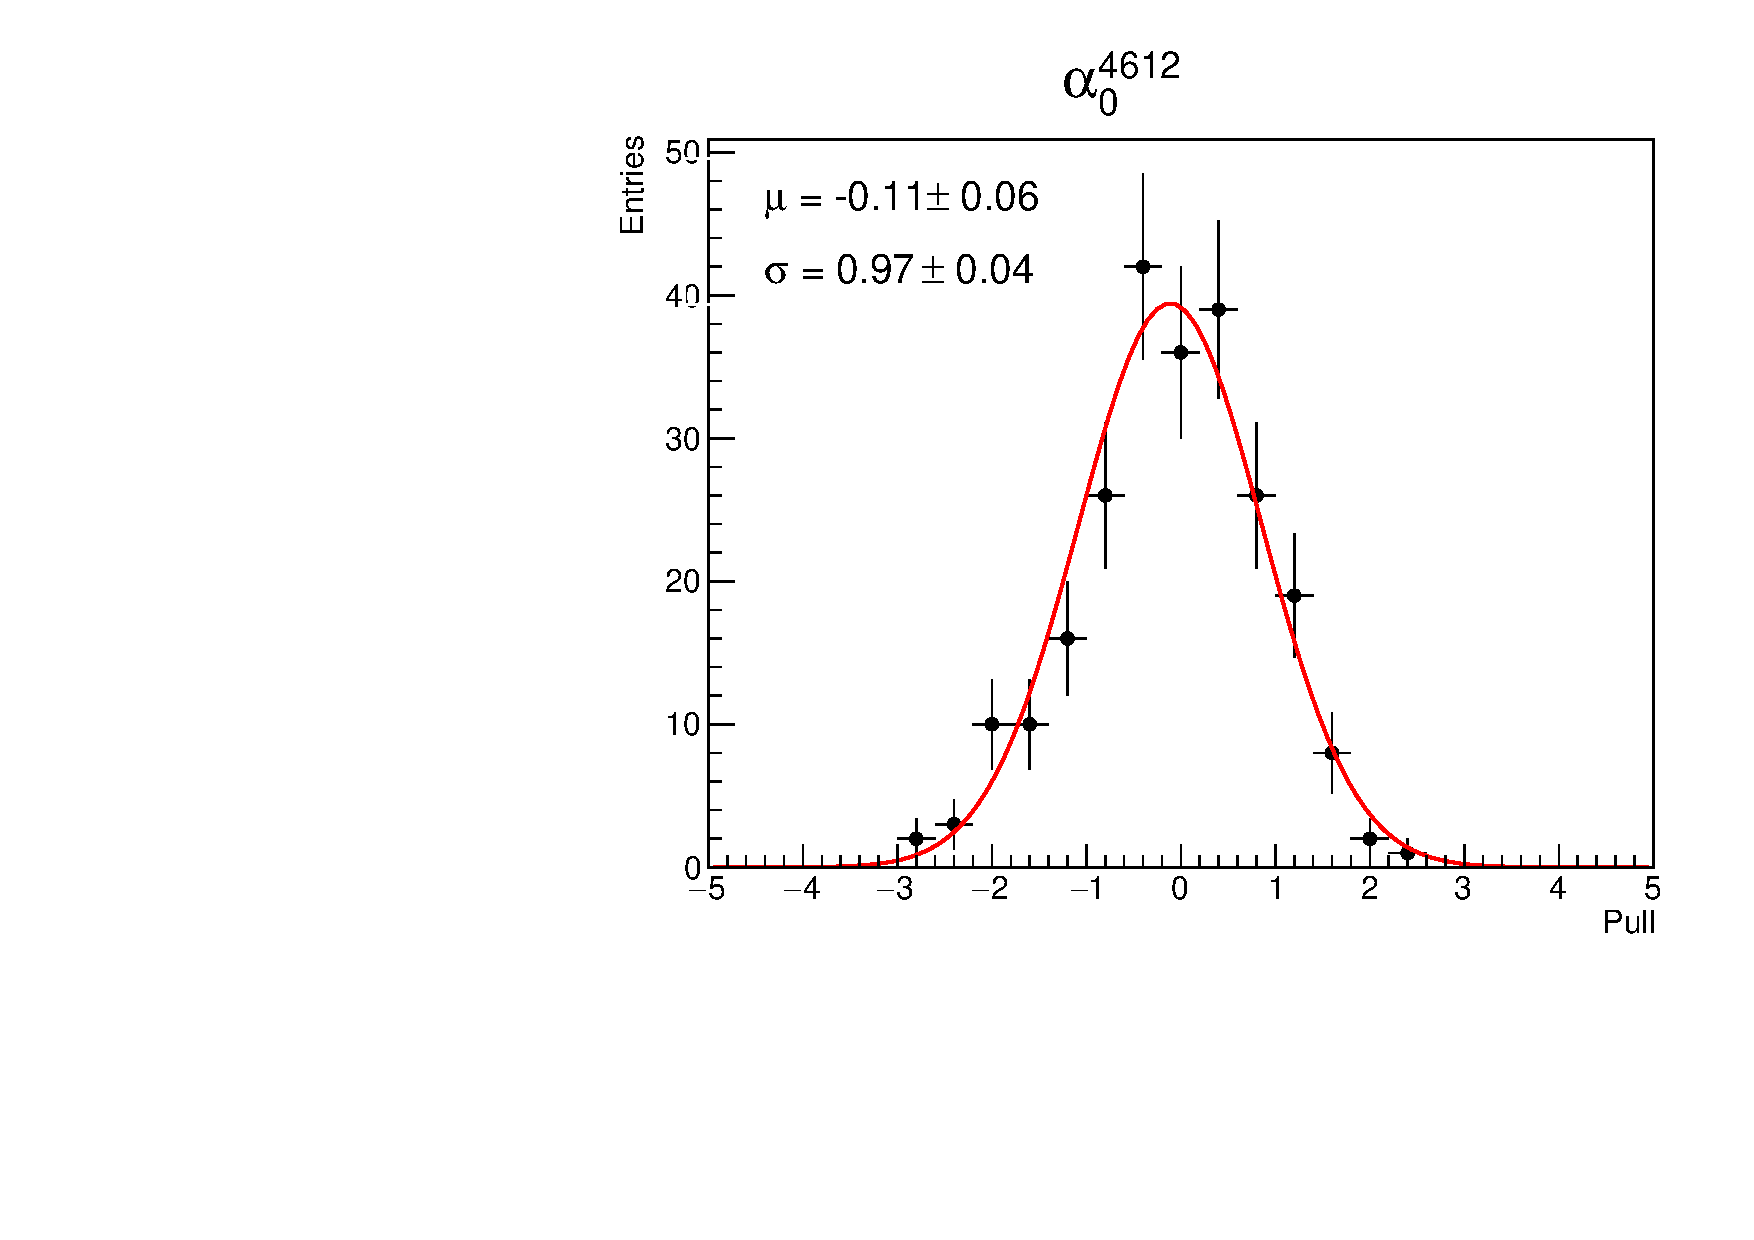
\includegraphics[width=0.24\textwidth]{figure/io_full_sim/polarization/pull_polarization_alpha0_4612.pdf}
    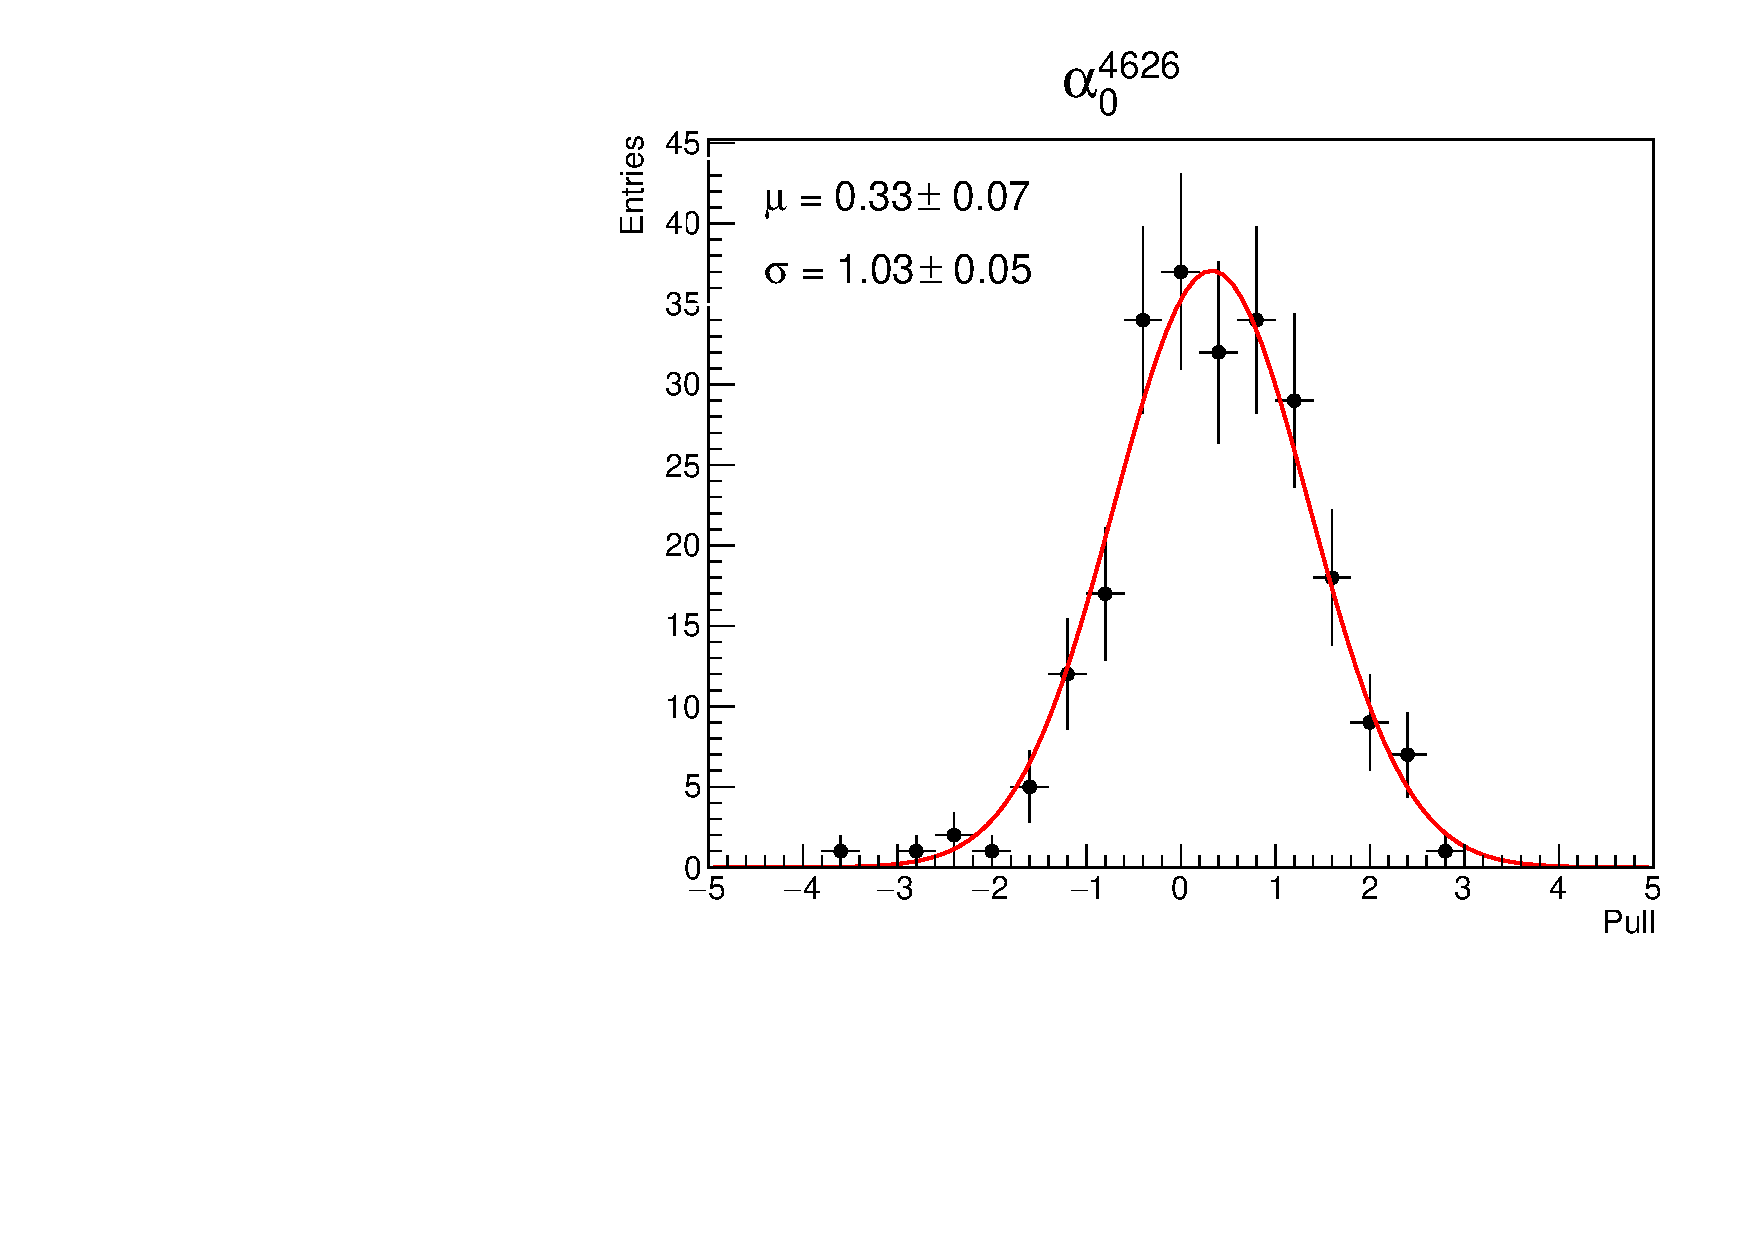
\includegraphics[width=0.24\textwidth]{figure/io_full_sim/polarization/pull_polarization_alpha0_4626.pdf}
    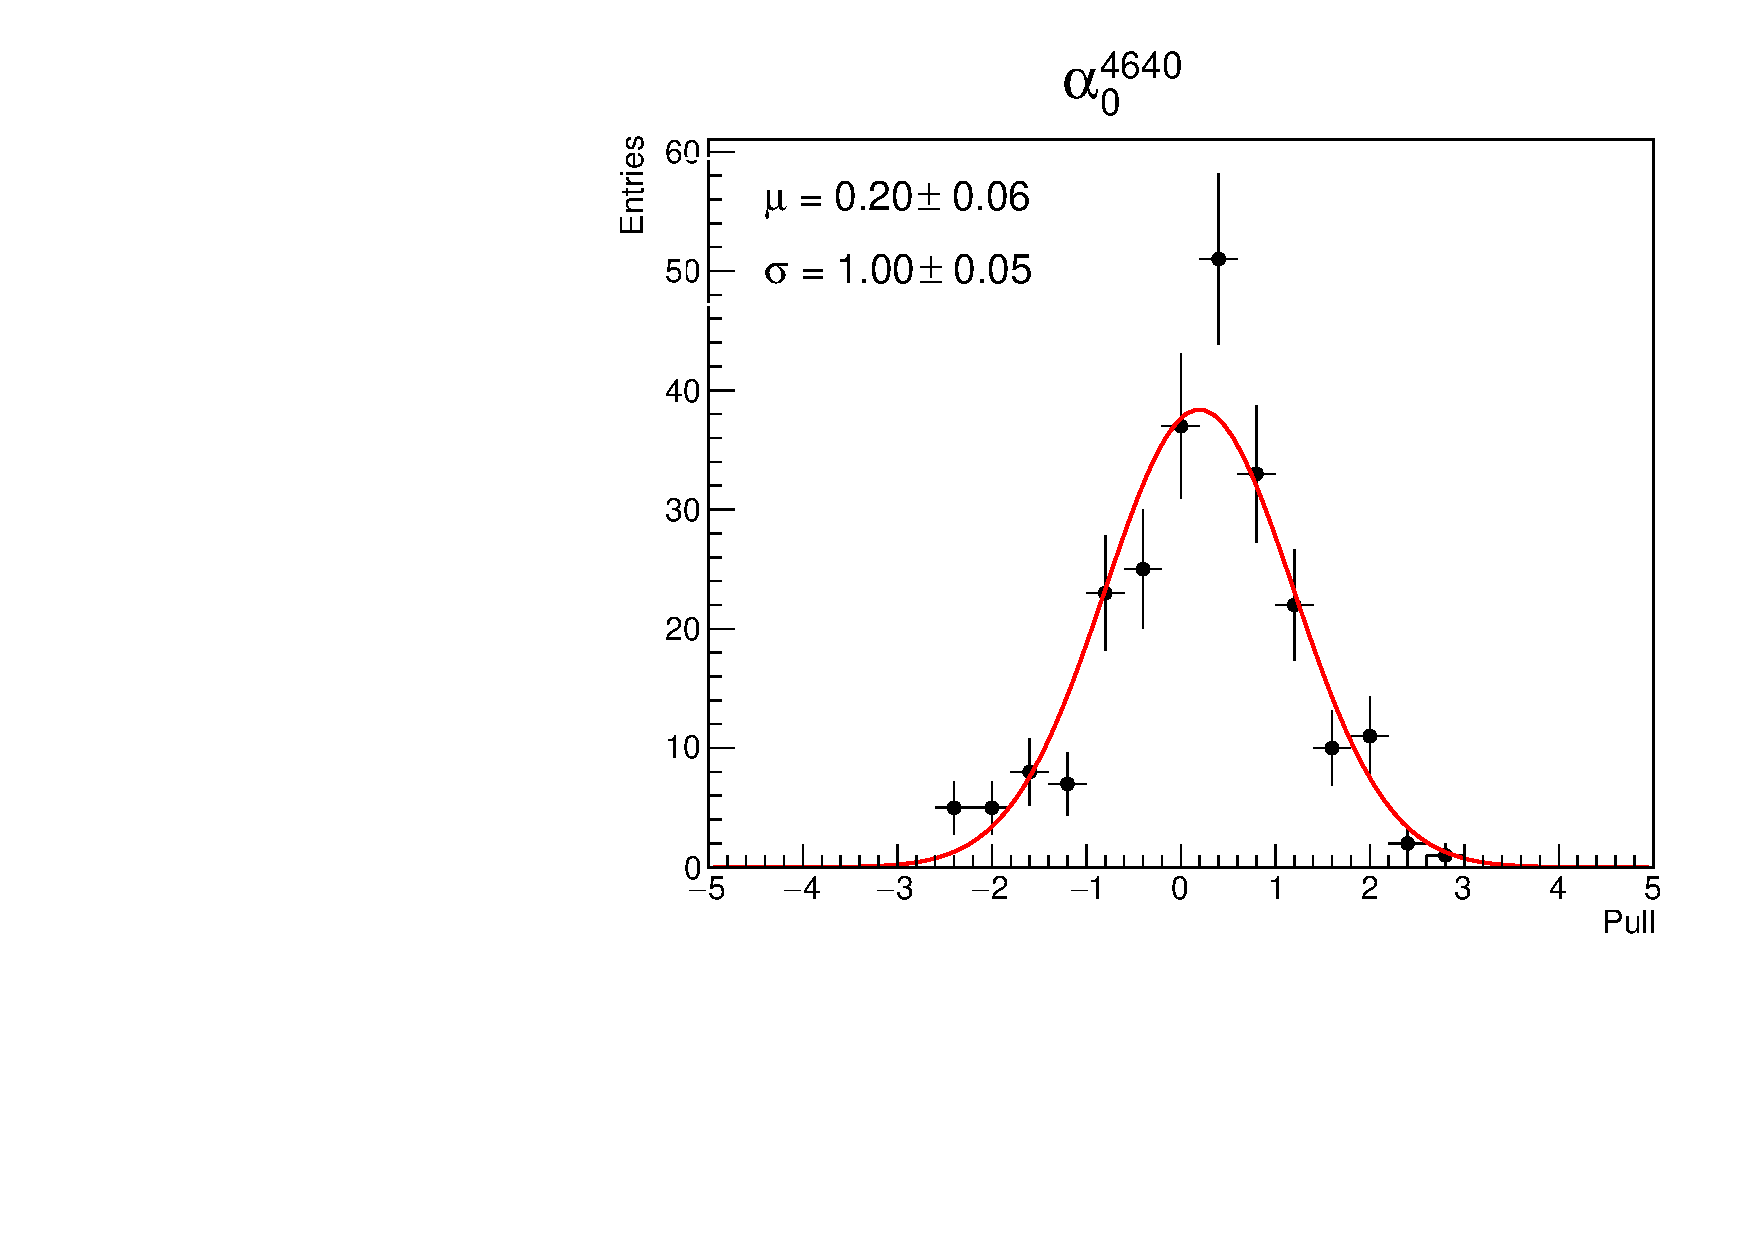
\includegraphics[width=0.24\textwidth]{figure/io_full_sim/polarization/pull_polarization_alpha0_4640.pdf}
    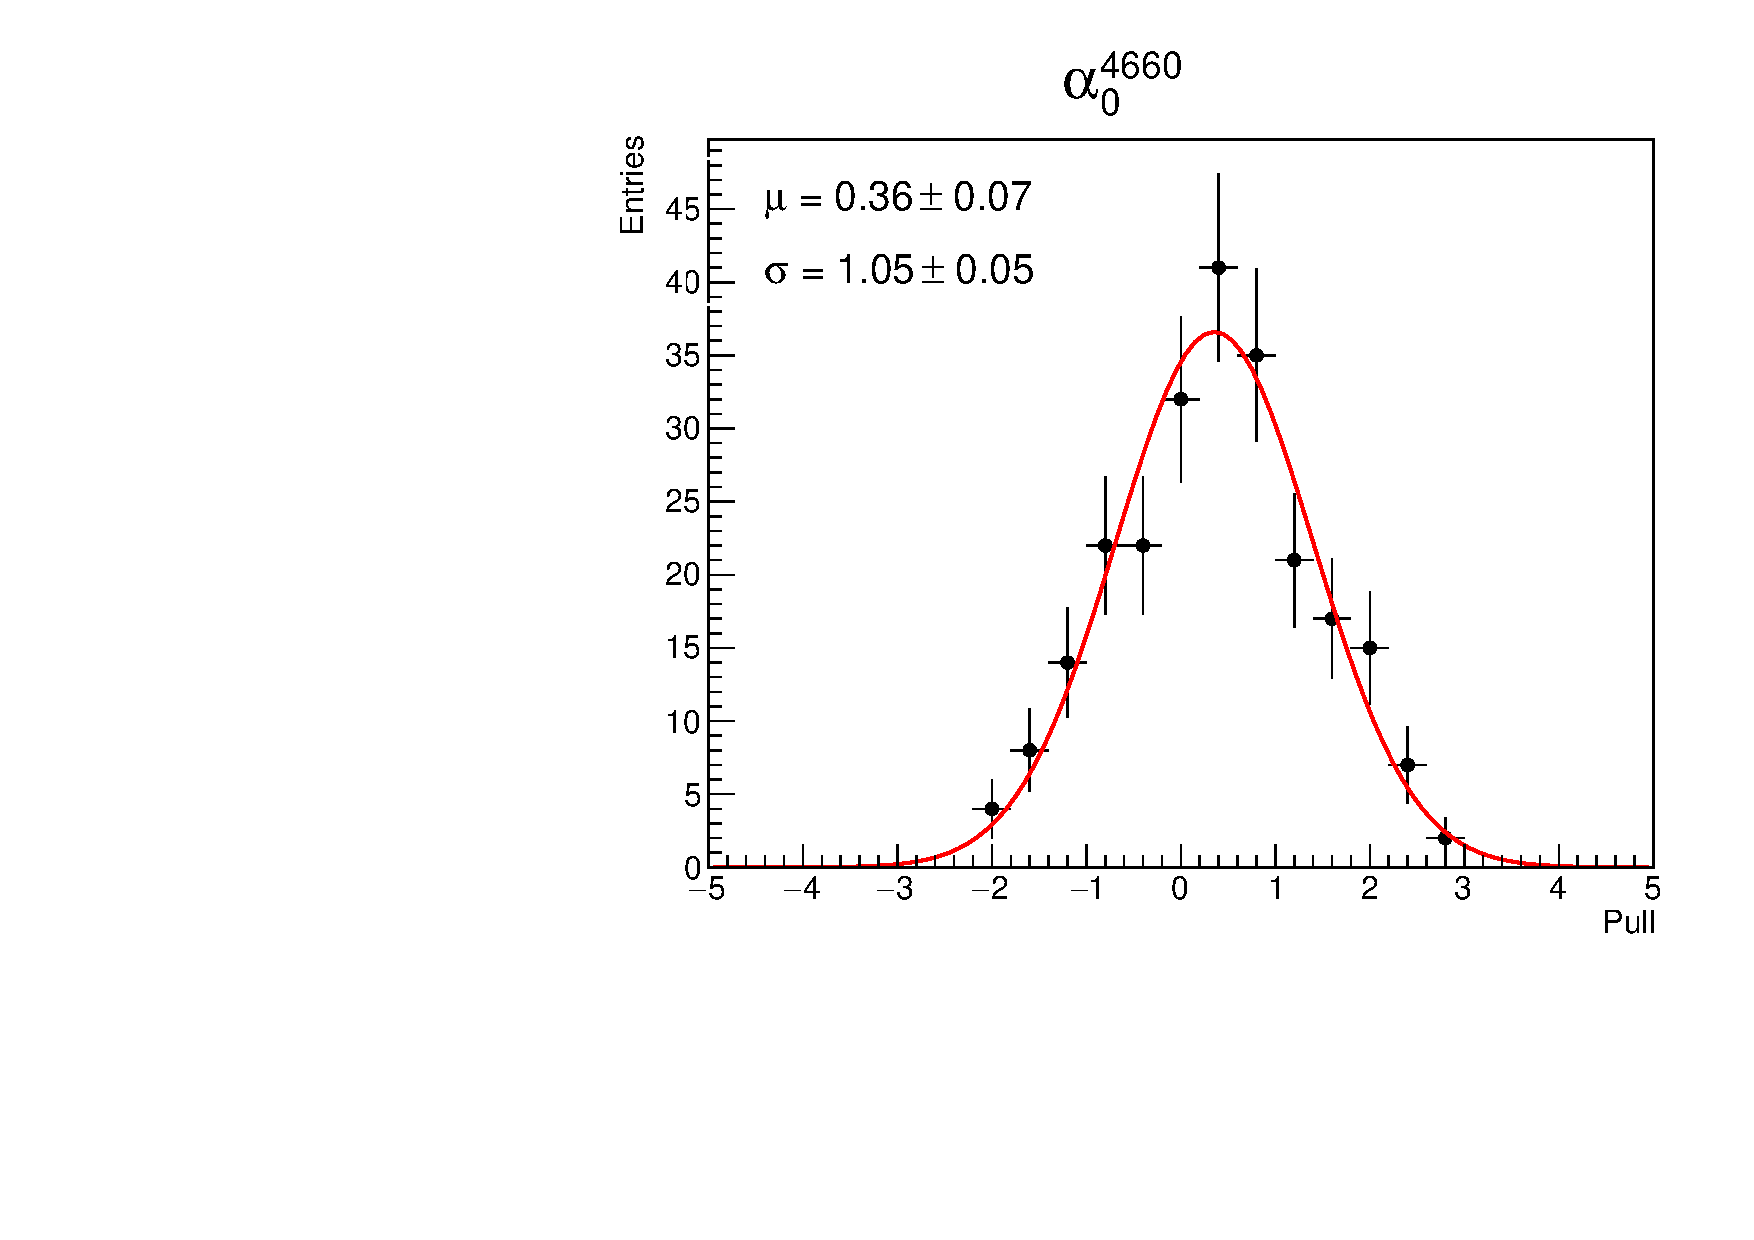
\includegraphics[width=0.24\textwidth]{figure/io_full_sim/polarization/pull_polarization_alpha0_4660.pdf}
    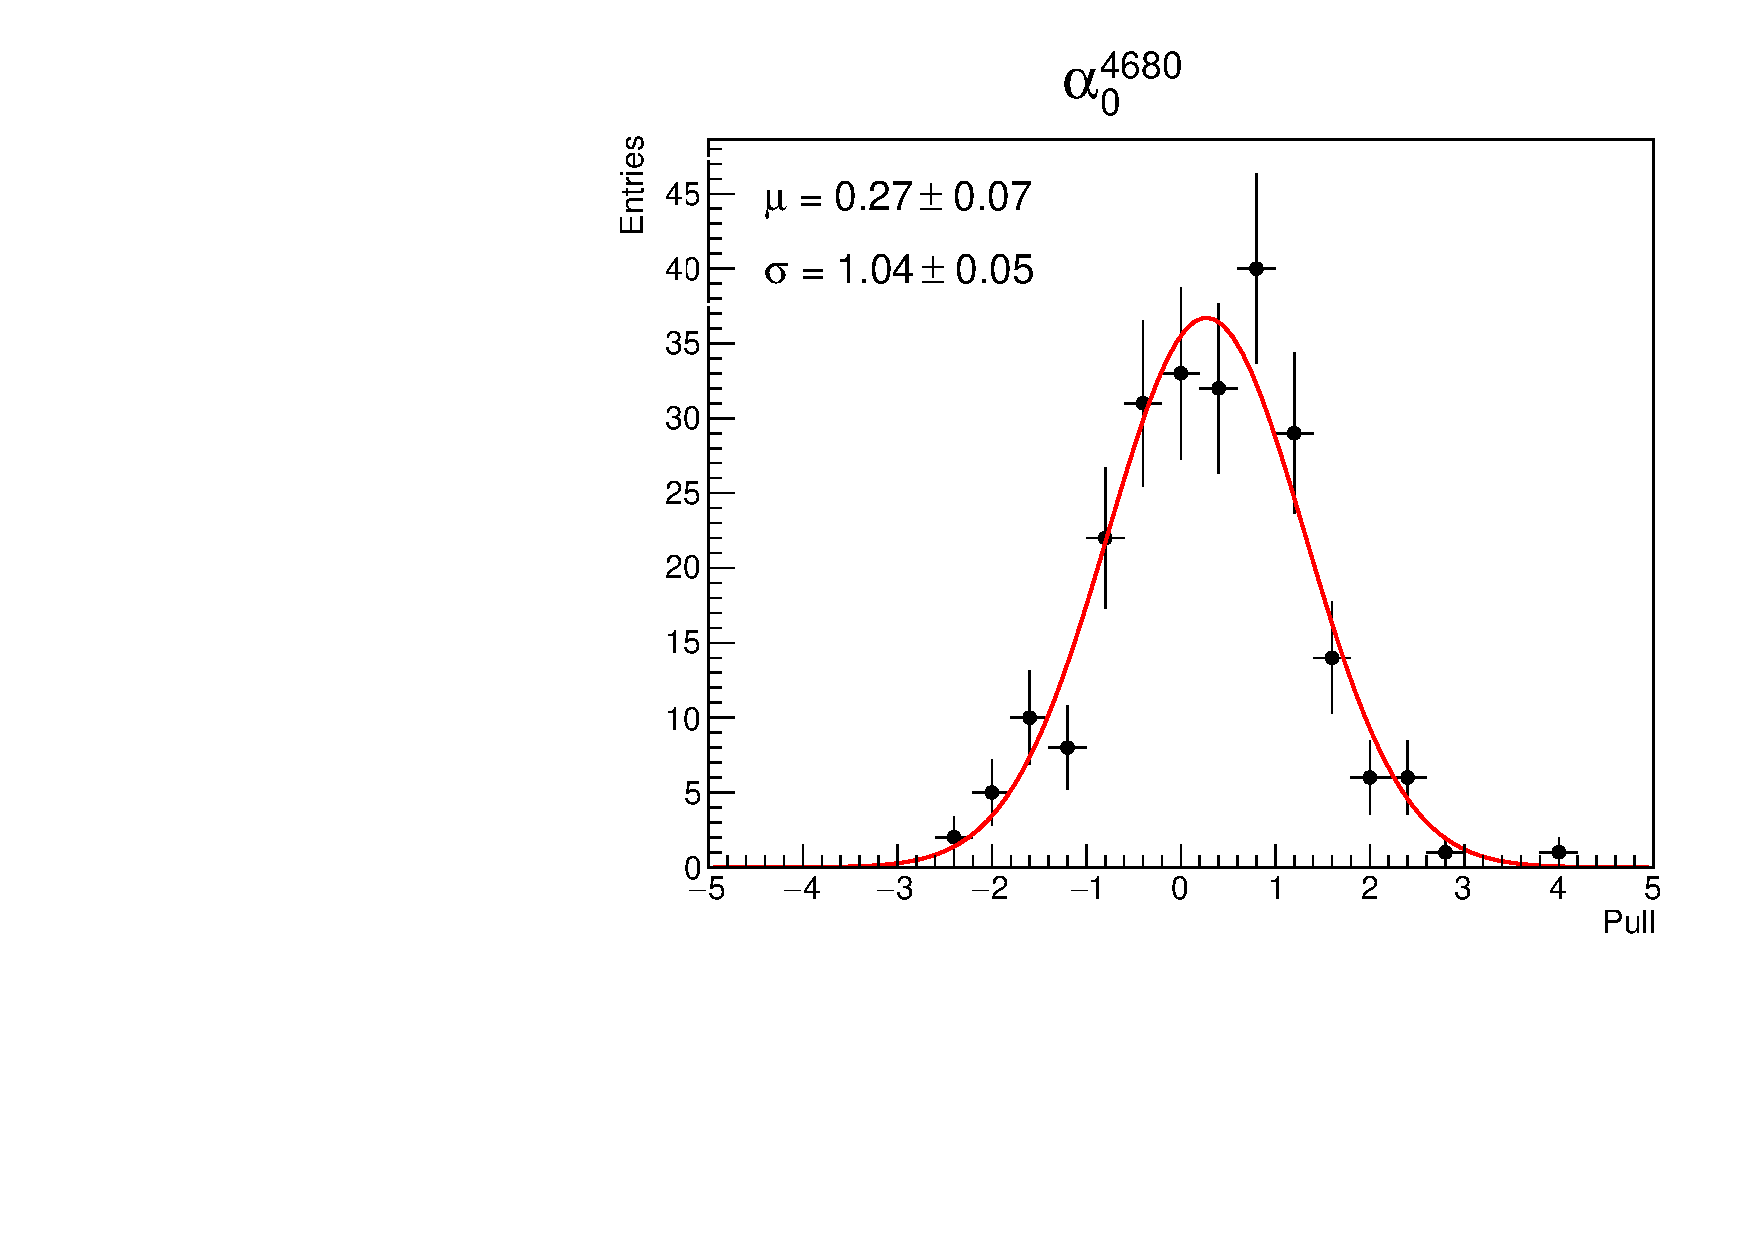
\includegraphics[width=0.24\textwidth]{figure/io_full_sim/polarization/pull_polarization_alpha0_4680.pdf}
    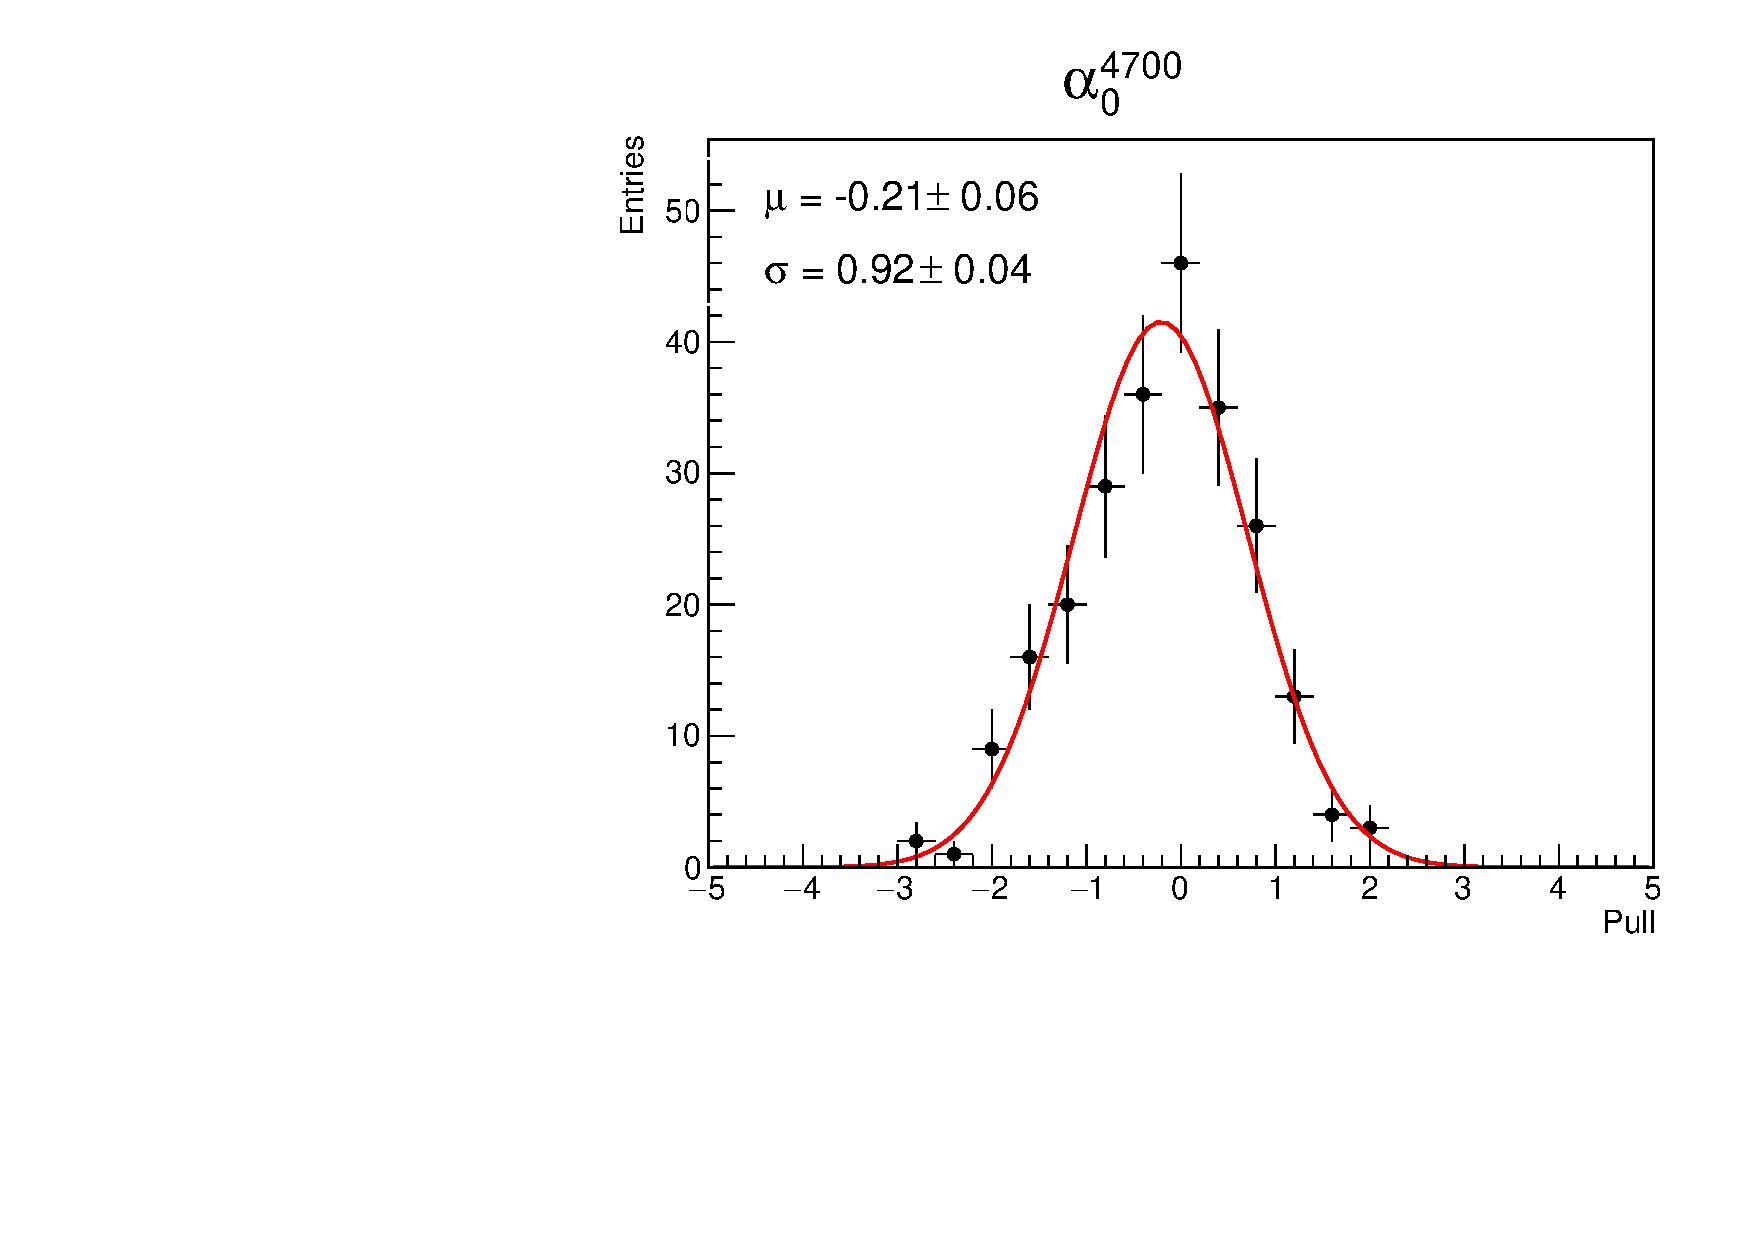
\includegraphics[width=0.24\textwidth]{figure/io_full_sim/polarization/pull_polarization_alpha0_4700.pdf}
    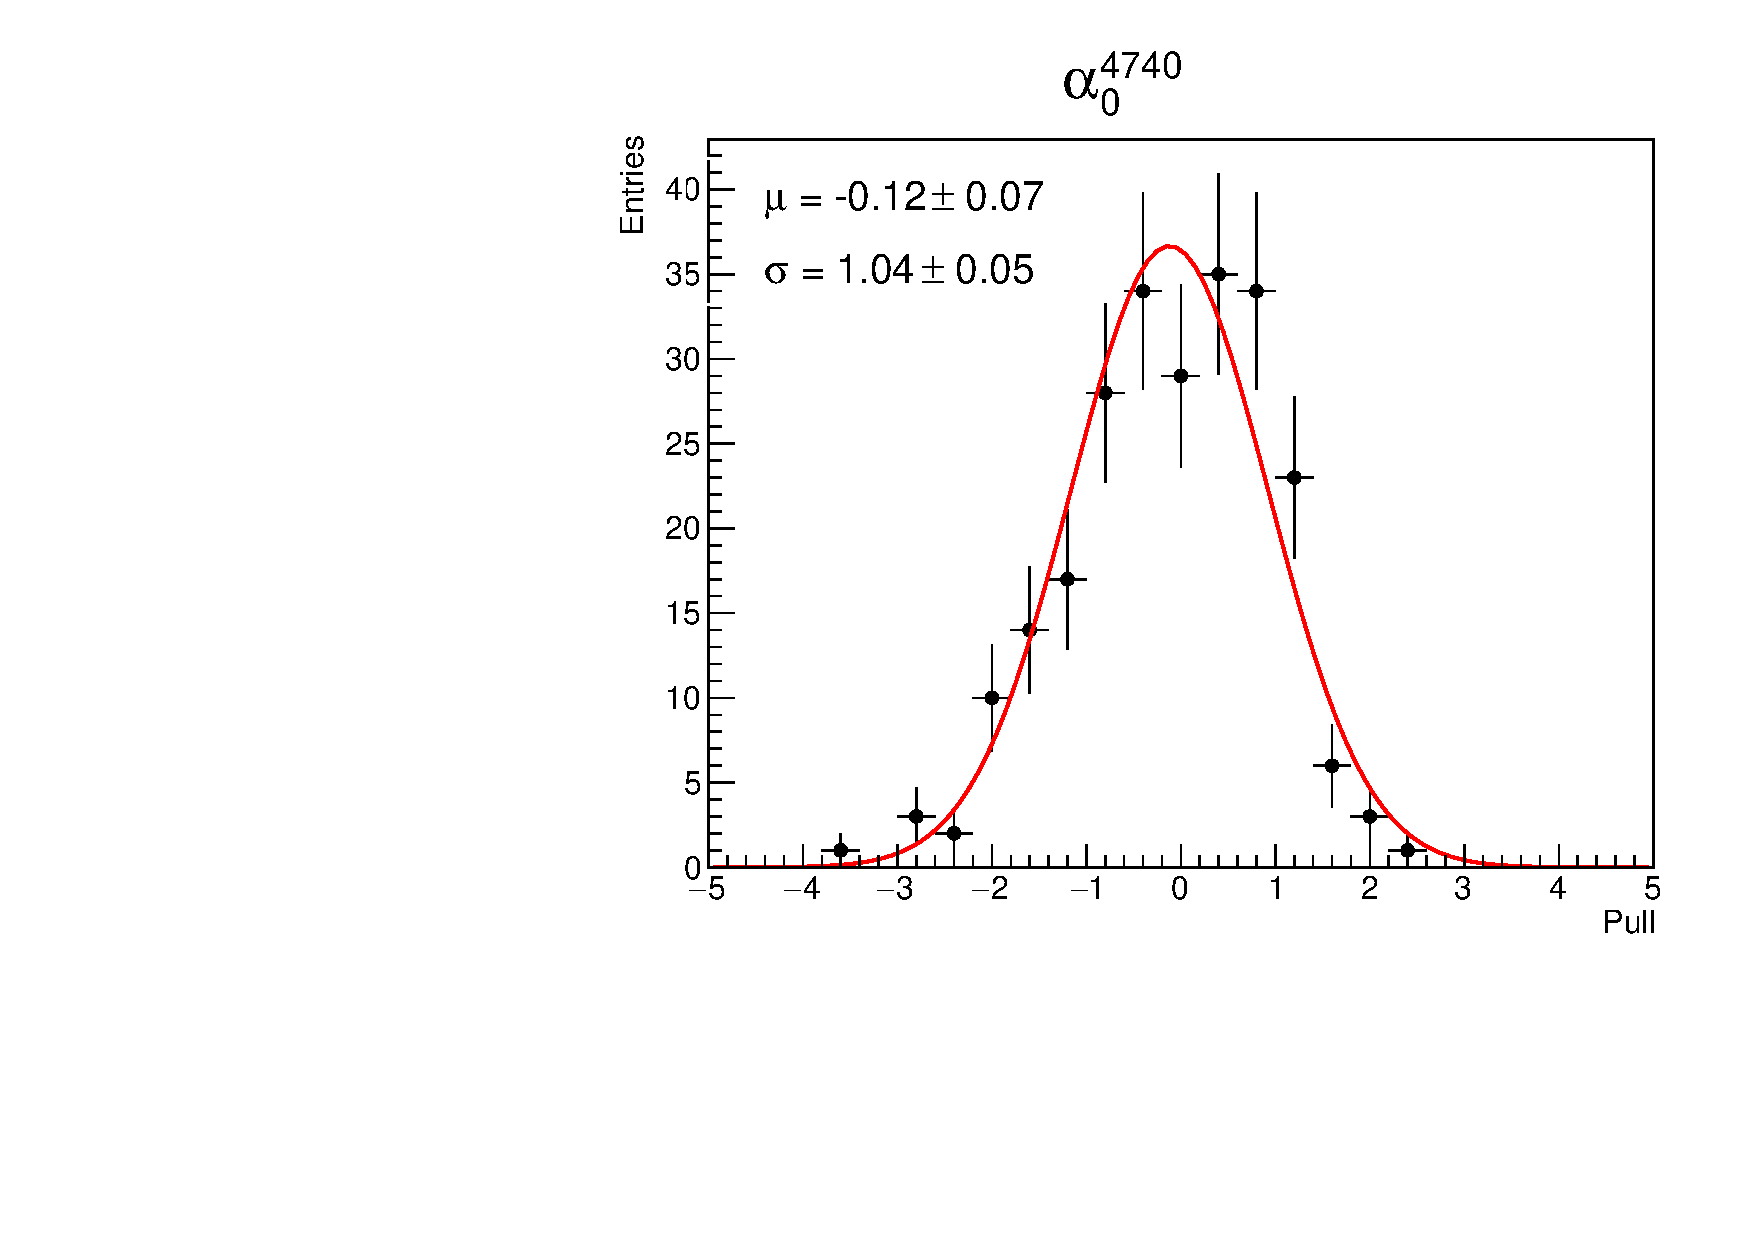
\includegraphics[width=0.24\textwidth]{figure/io_full_sim/polarization/pull_polarization_alpha0_4740.pdf}
    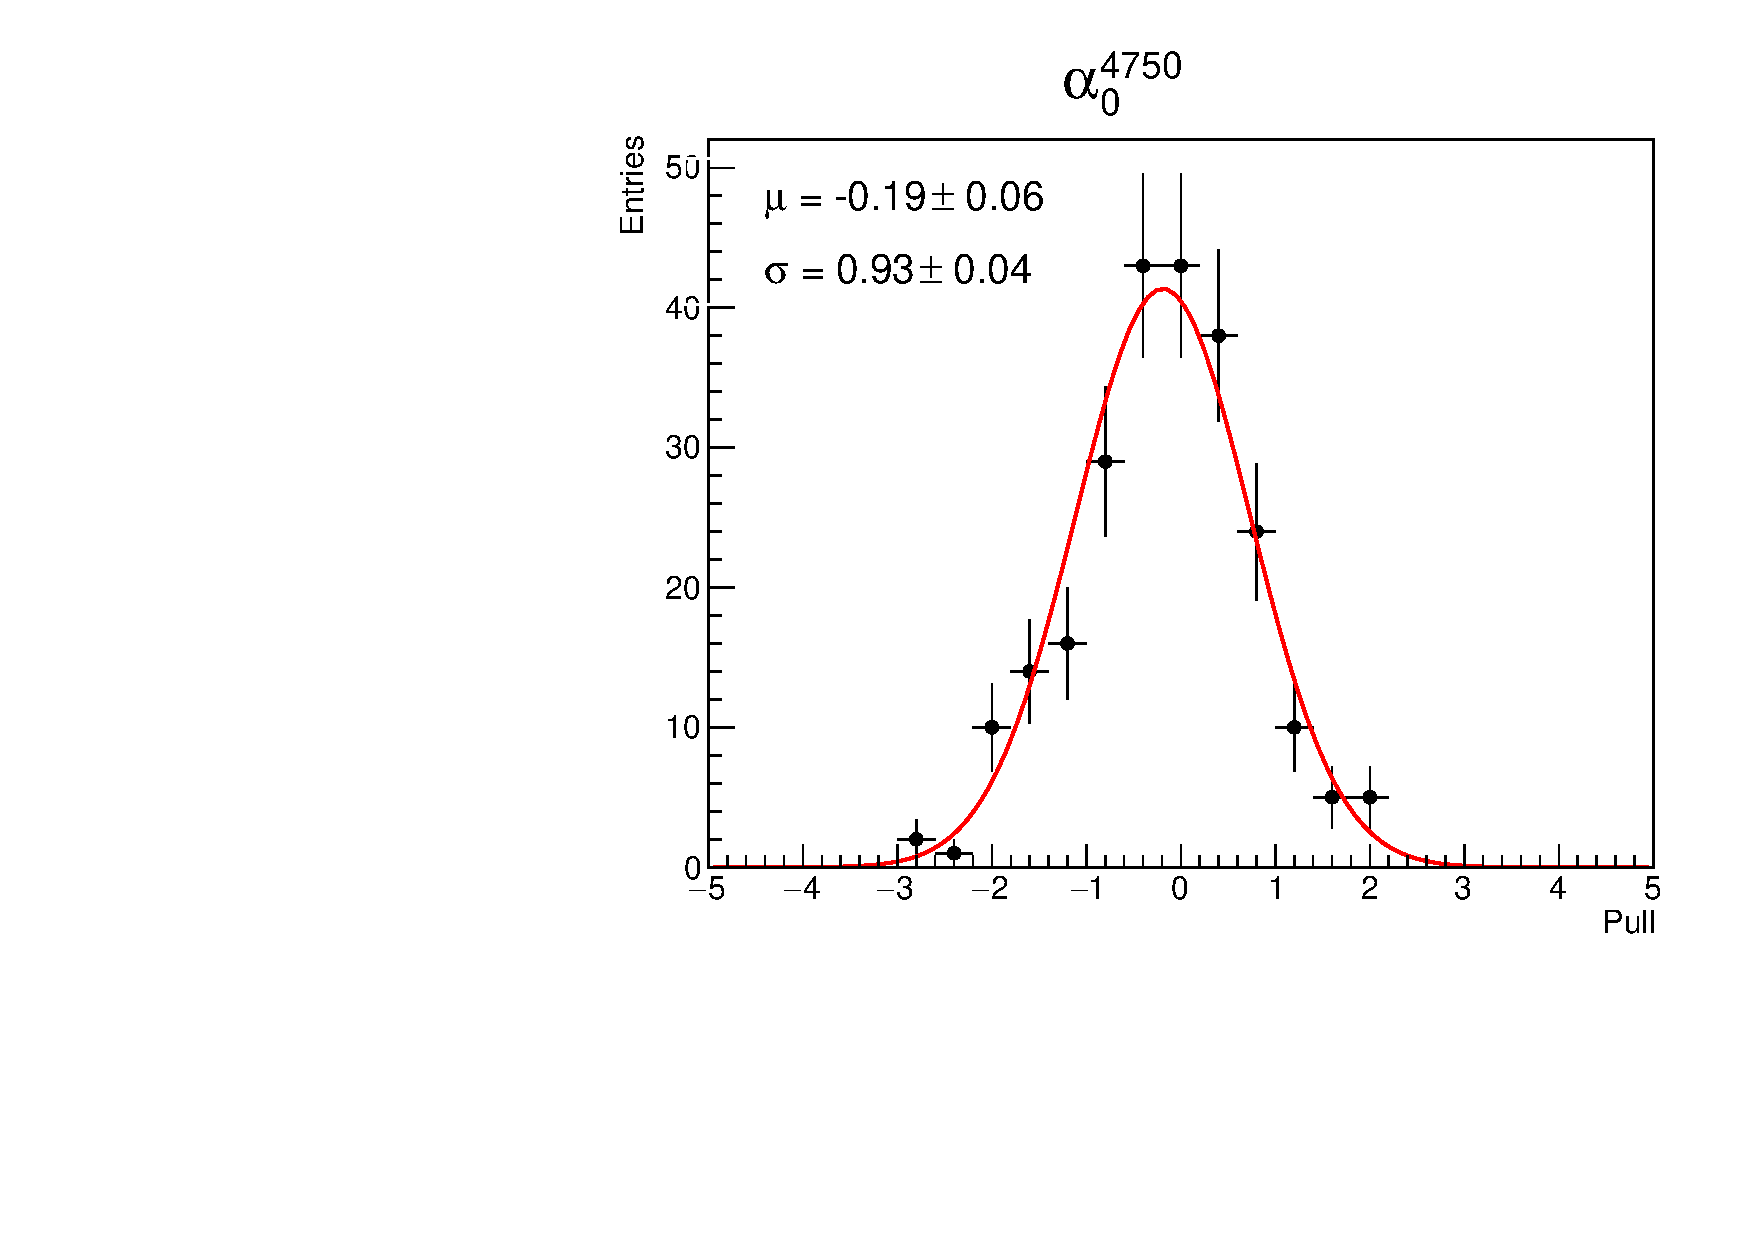
\includegraphics[width=0.24\textwidth]{figure/io_full_sim/polarization/pull_polarization_alpha0_4750.pdf}
    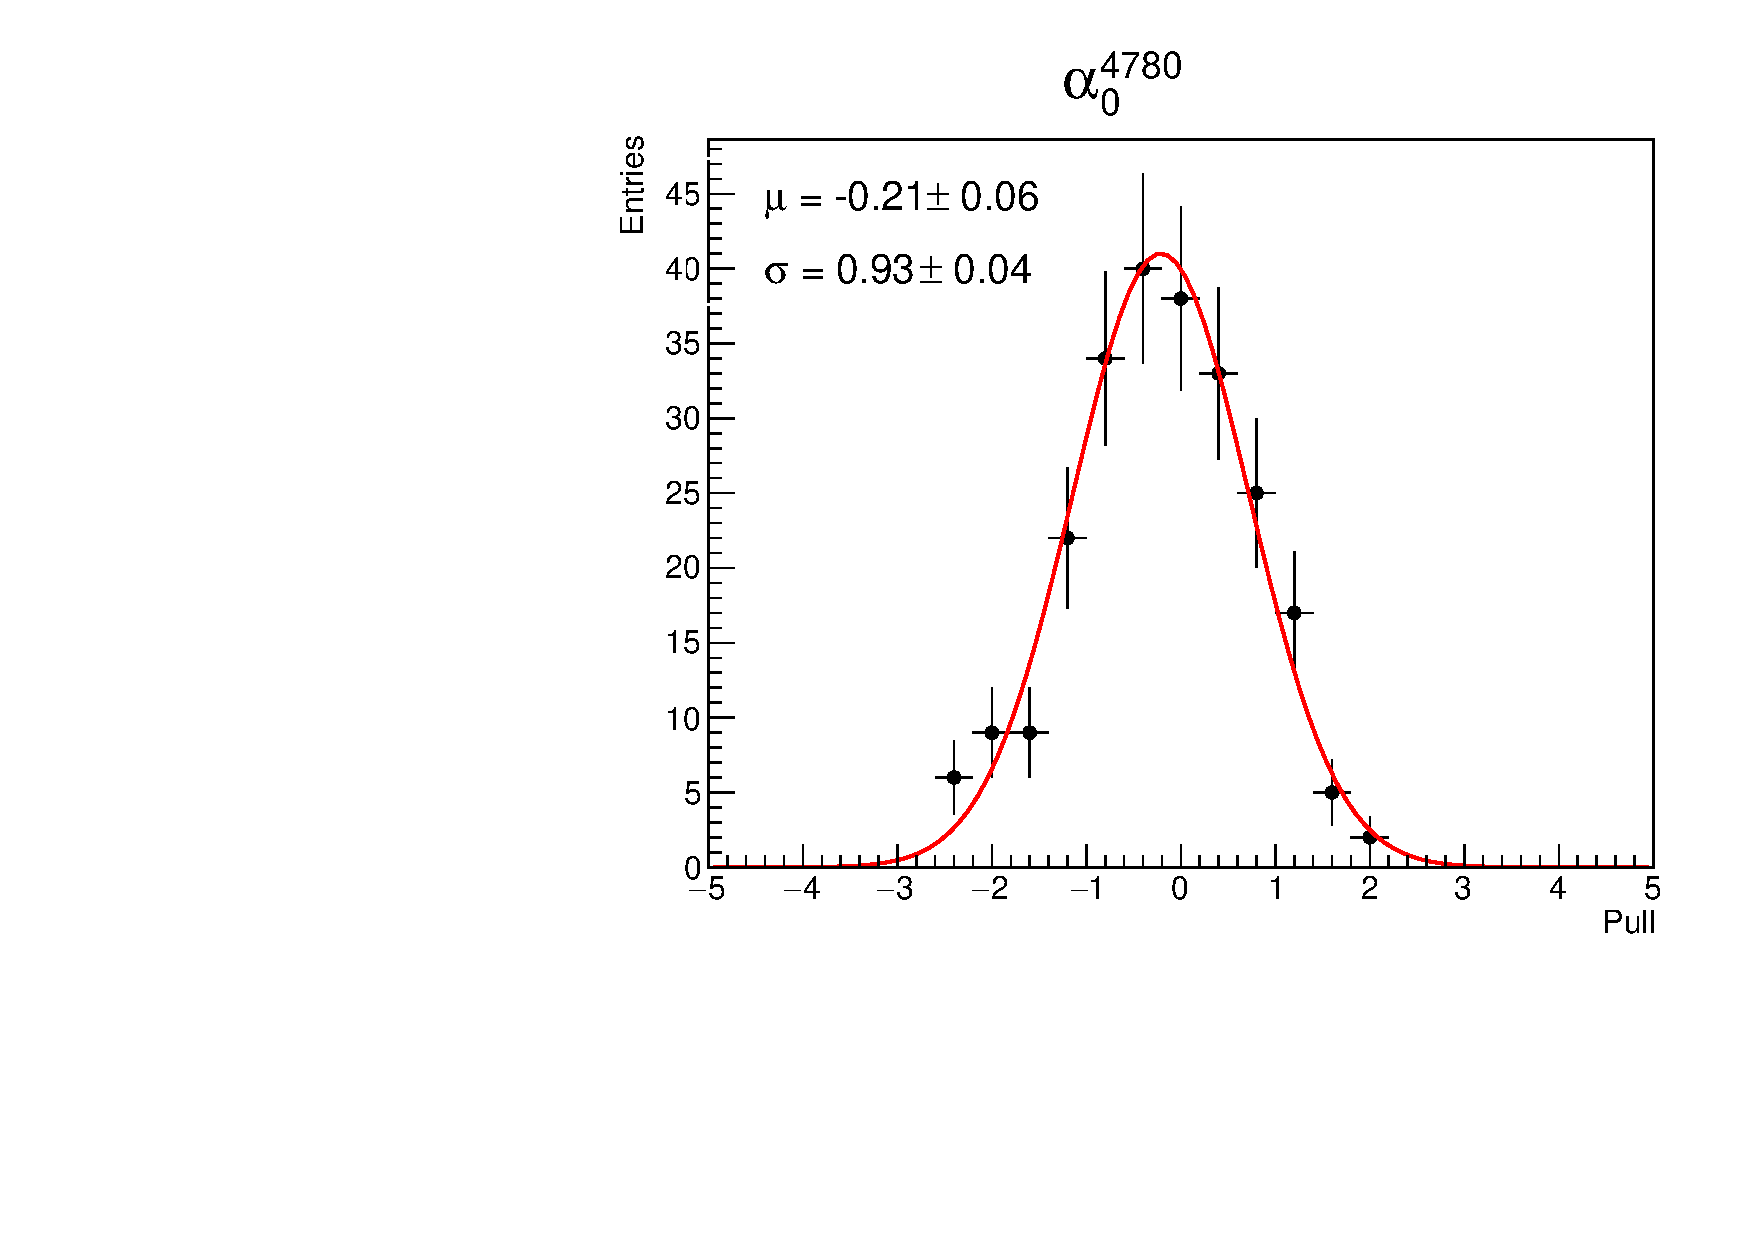
\includegraphics[width=0.24\textwidth]{figure/io_full_sim/polarization/pull_polarization_alpha0_4780.pdf}
    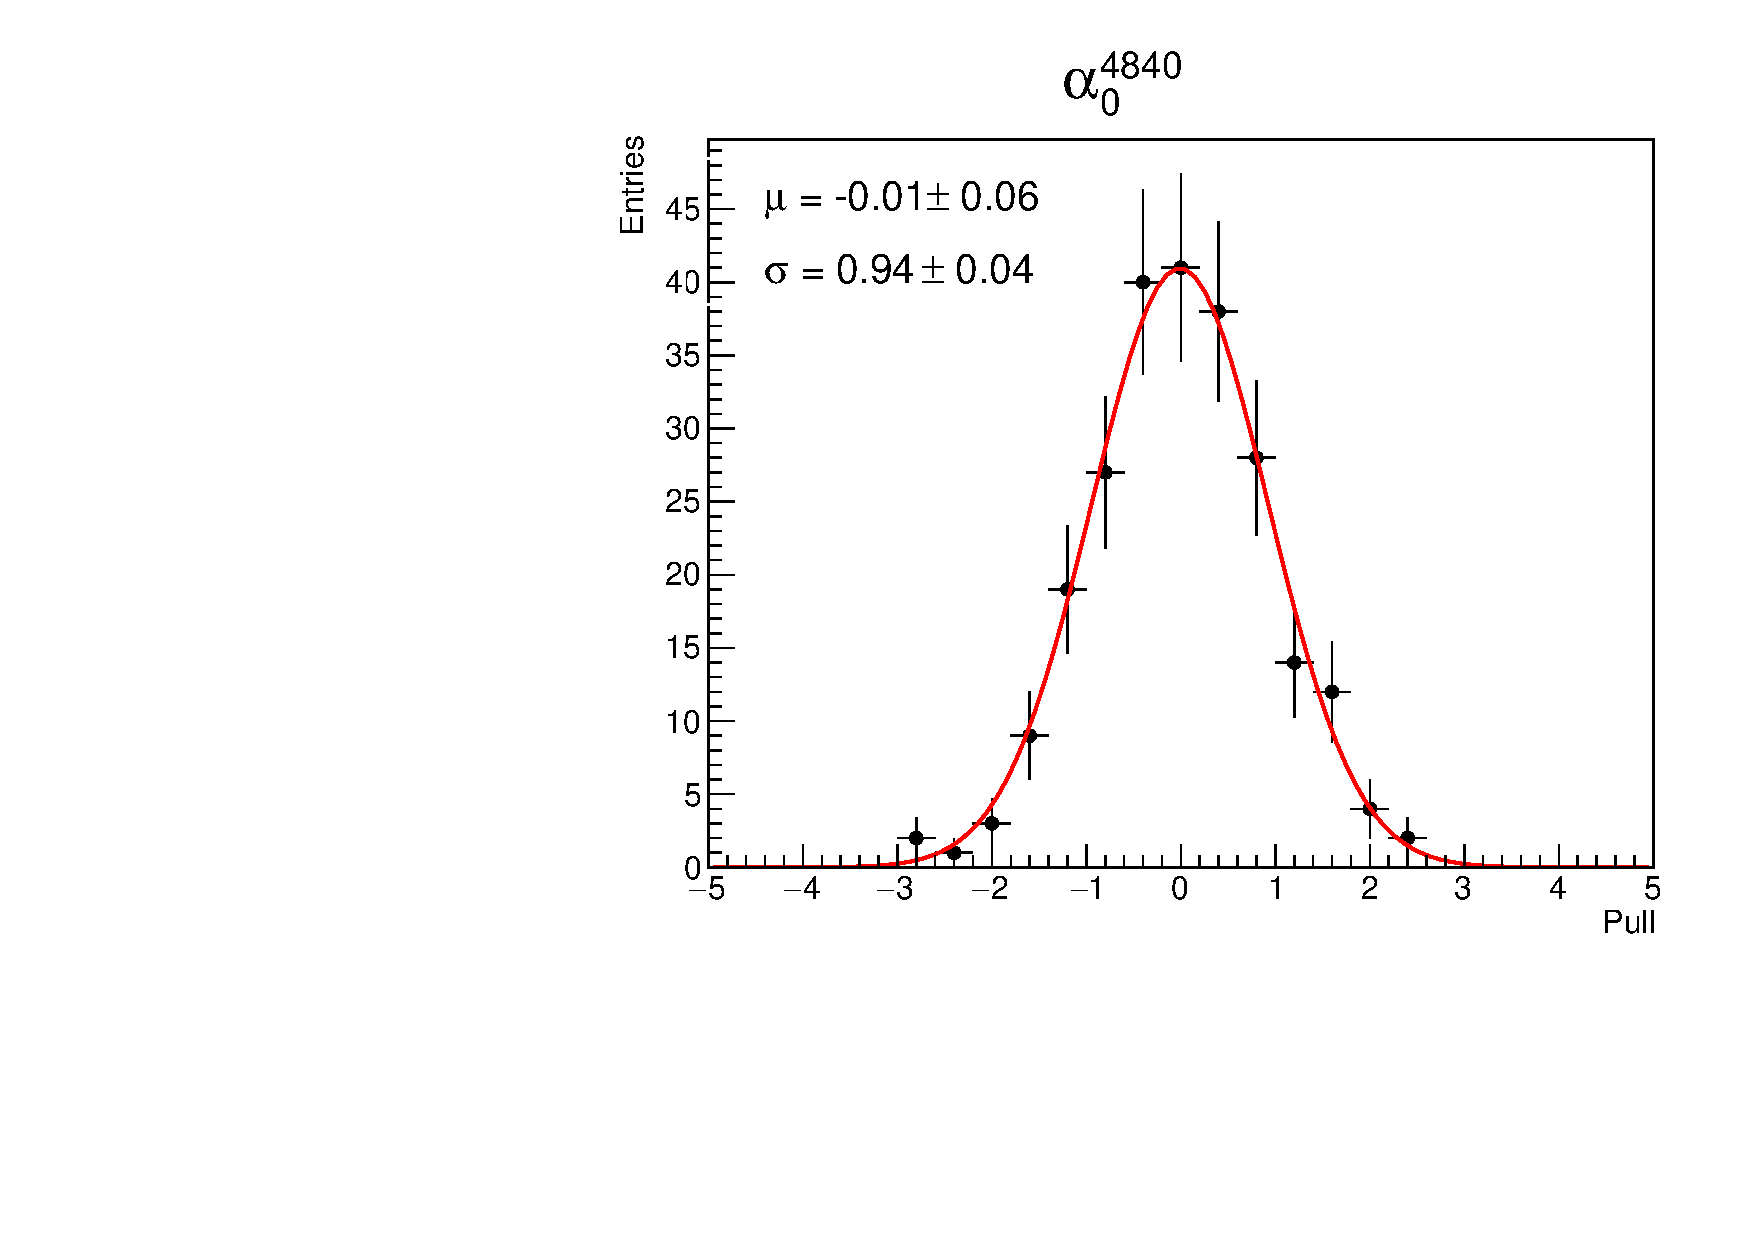
\includegraphics[width=0.24\textwidth]{figure/io_full_sim/polarization/pull_polarization_alpha0_4840.pdf}
    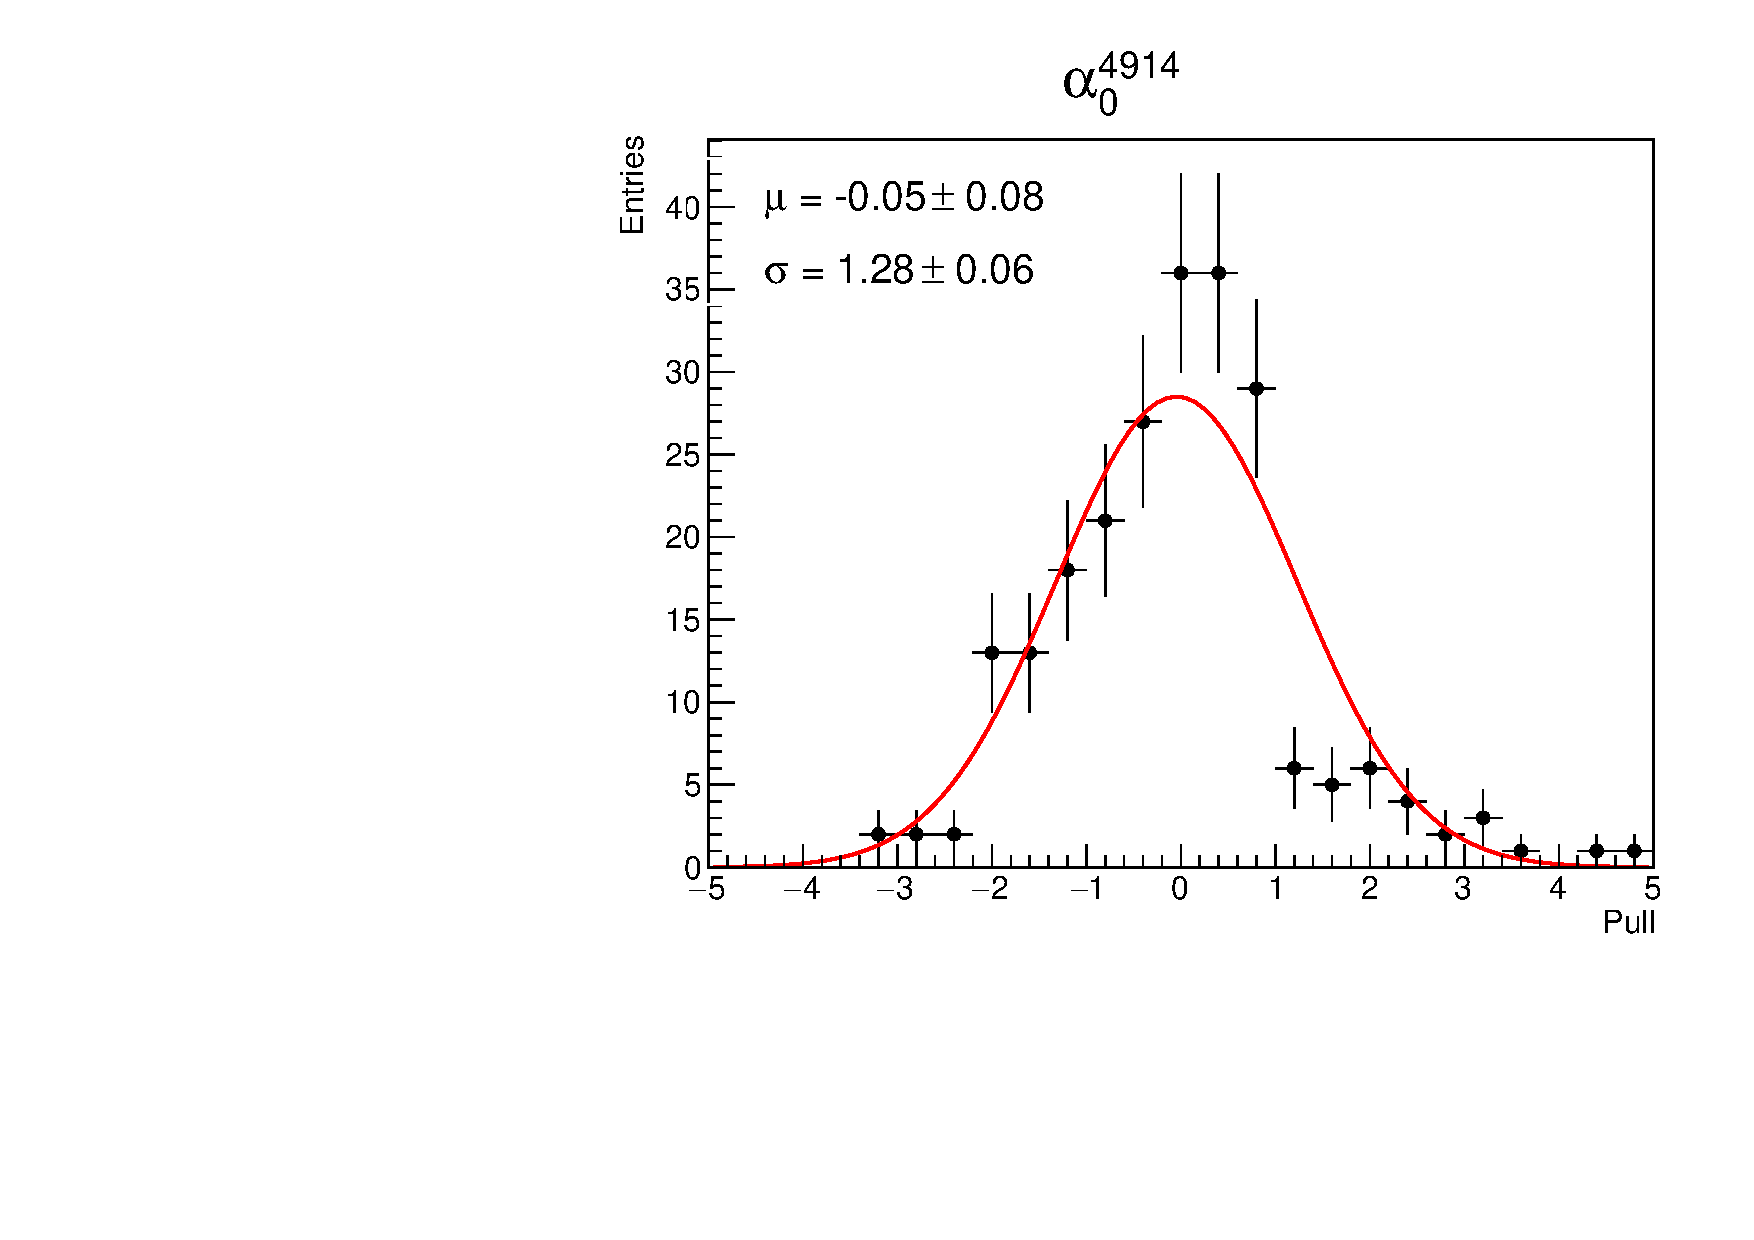
\includegraphics[width=0.24\textwidth]{figure/io_full_sim/polarization/pull_polarization_alpha0_4914.pdf}
    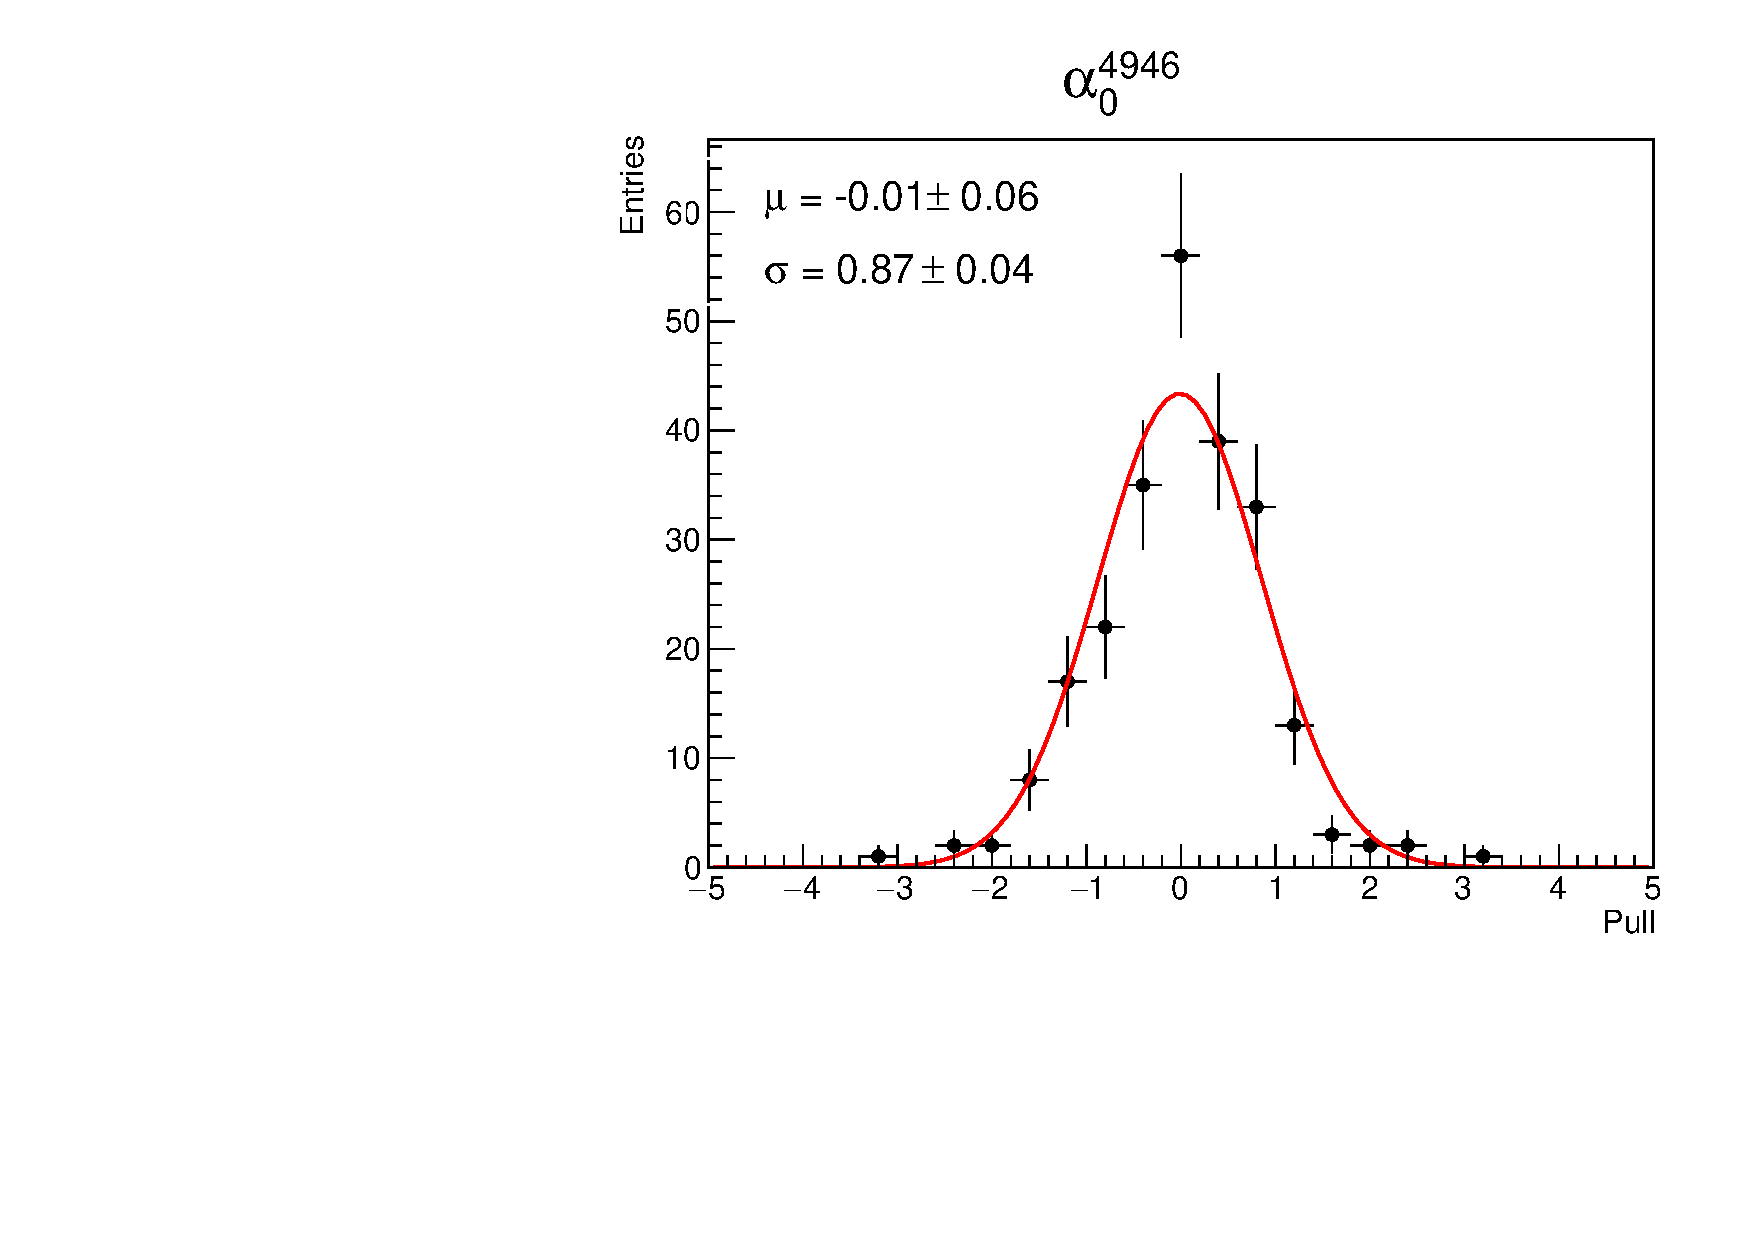
\includegraphics[width=0.24\textwidth]{figure/io_full_sim/polarization/pull_polarization_alpha0_4946.pdf}
    \caption{Pull distributions of $\alpha_0$ for each energy point.}
\label{fig:io_wo_bkg_pull_alpha0}
\end{figure}

\begin{figure}[h]\centering
    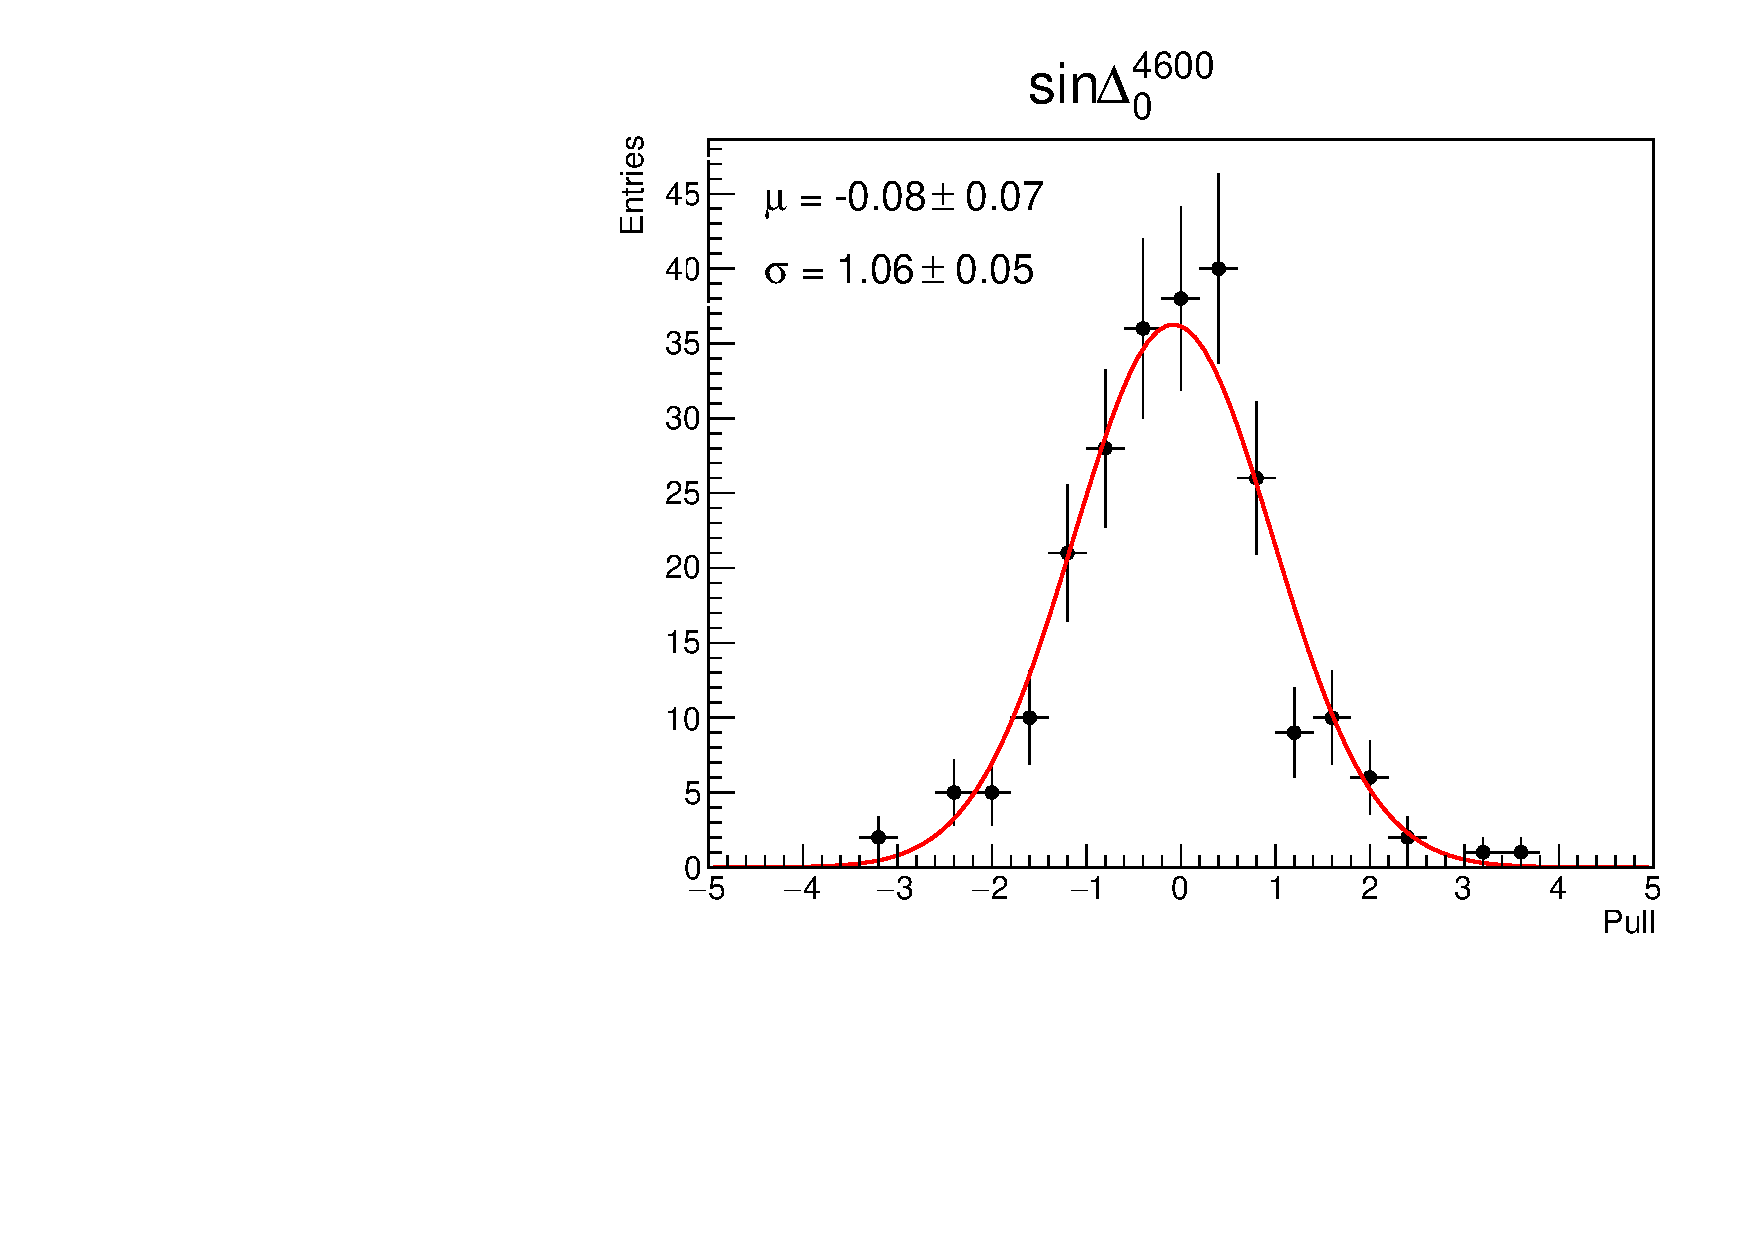
\includegraphics[width=0.24\textwidth]{figure/io_full_sim/polarization/pull_polarization_delta0_4600.pdf}
    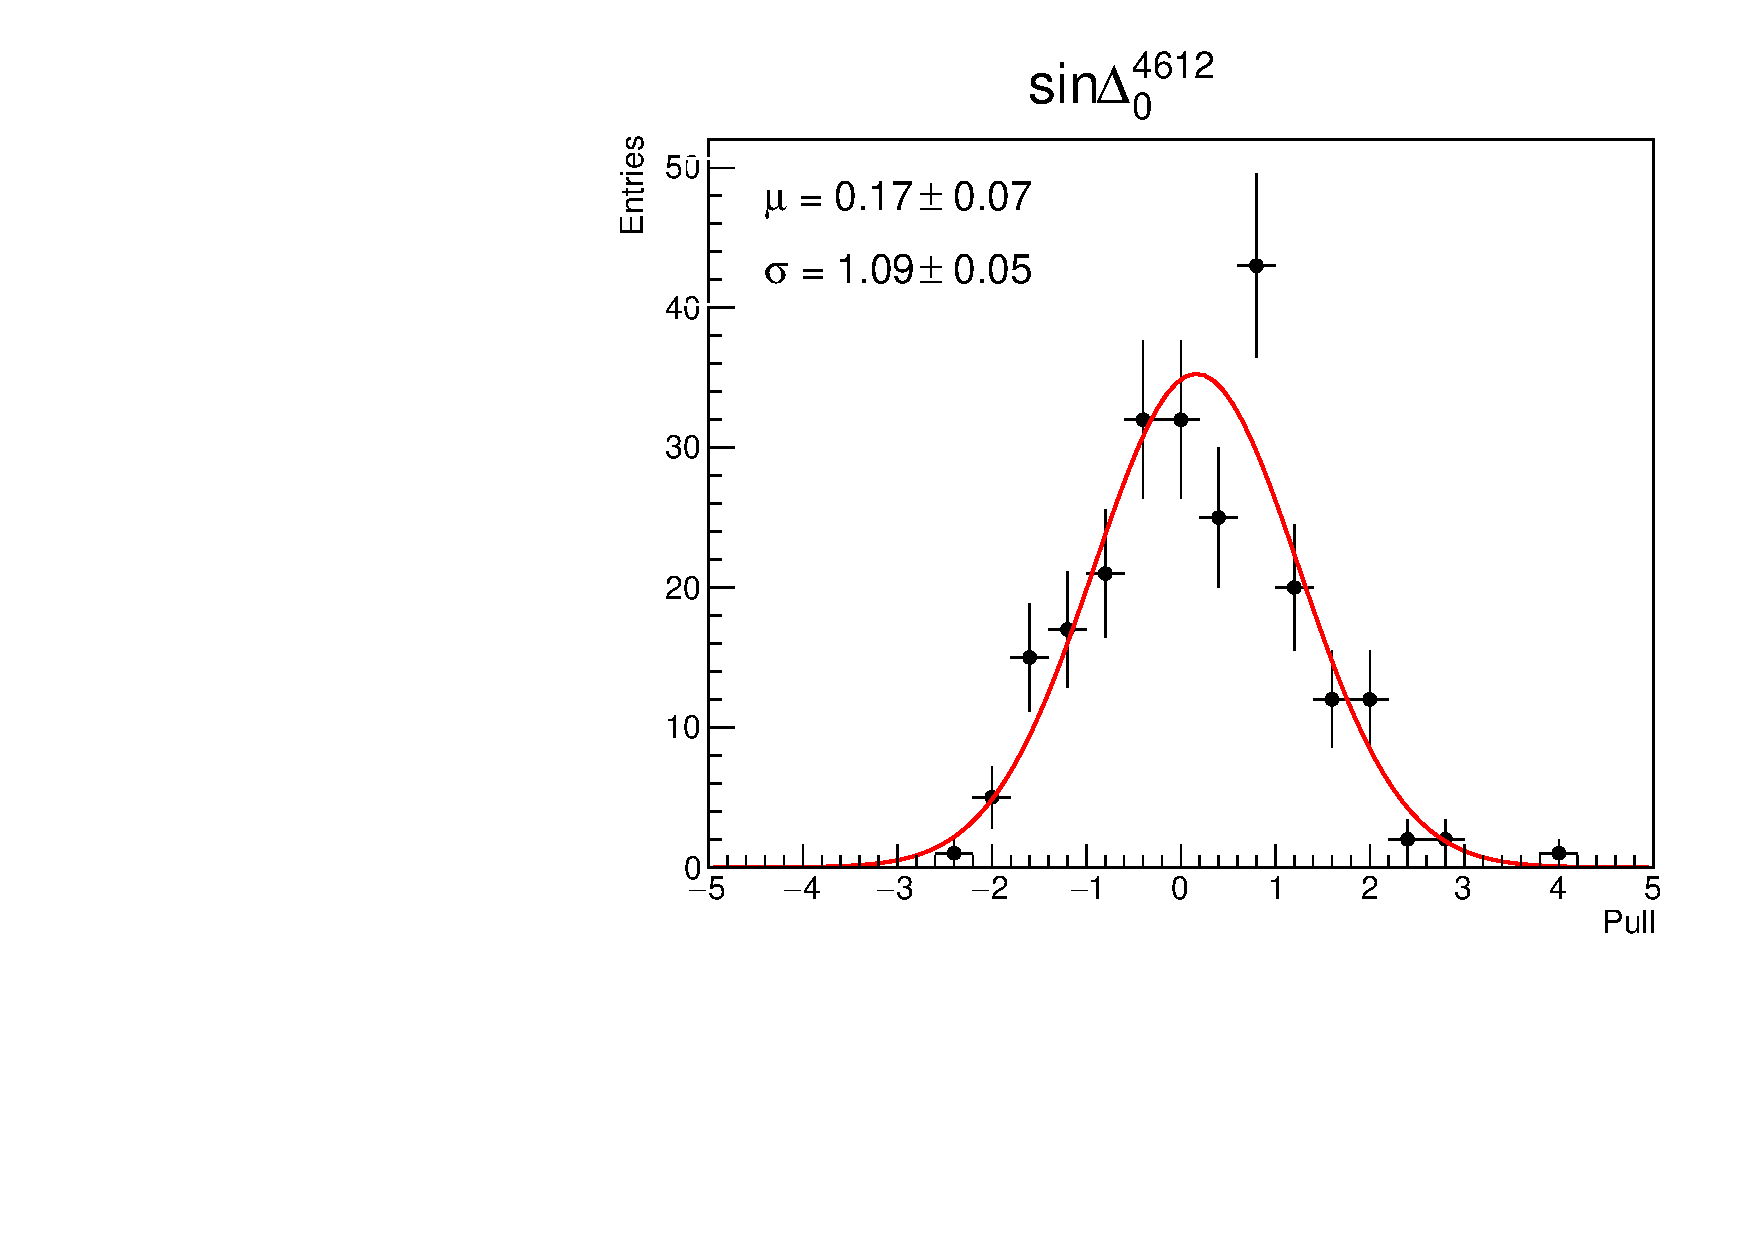
\includegraphics[width=0.24\textwidth]{figure/io_full_sim/polarization/pull_polarization_delta0_4612.pdf}
    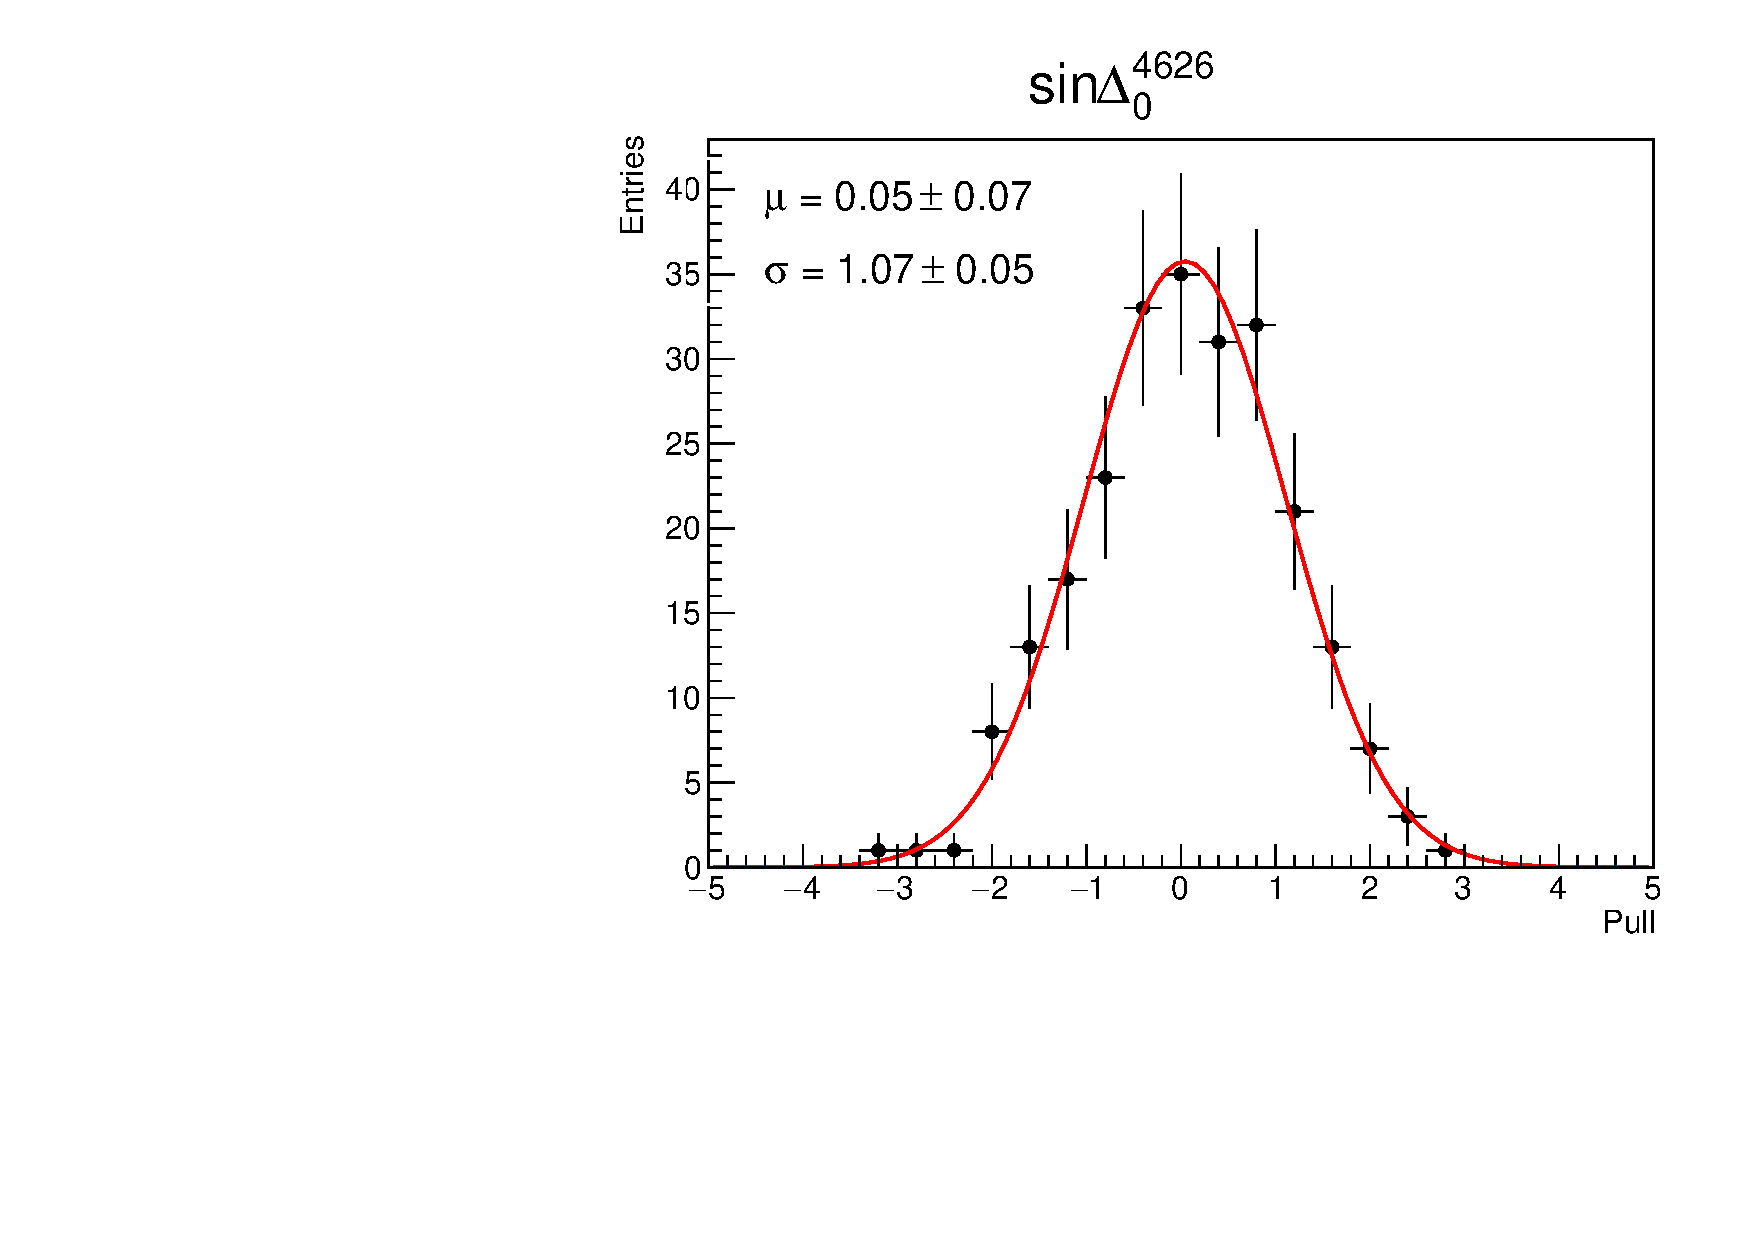
\includegraphics[width=0.24\textwidth]{figure/io_full_sim/polarization/pull_polarization_delta0_4626.pdf}
    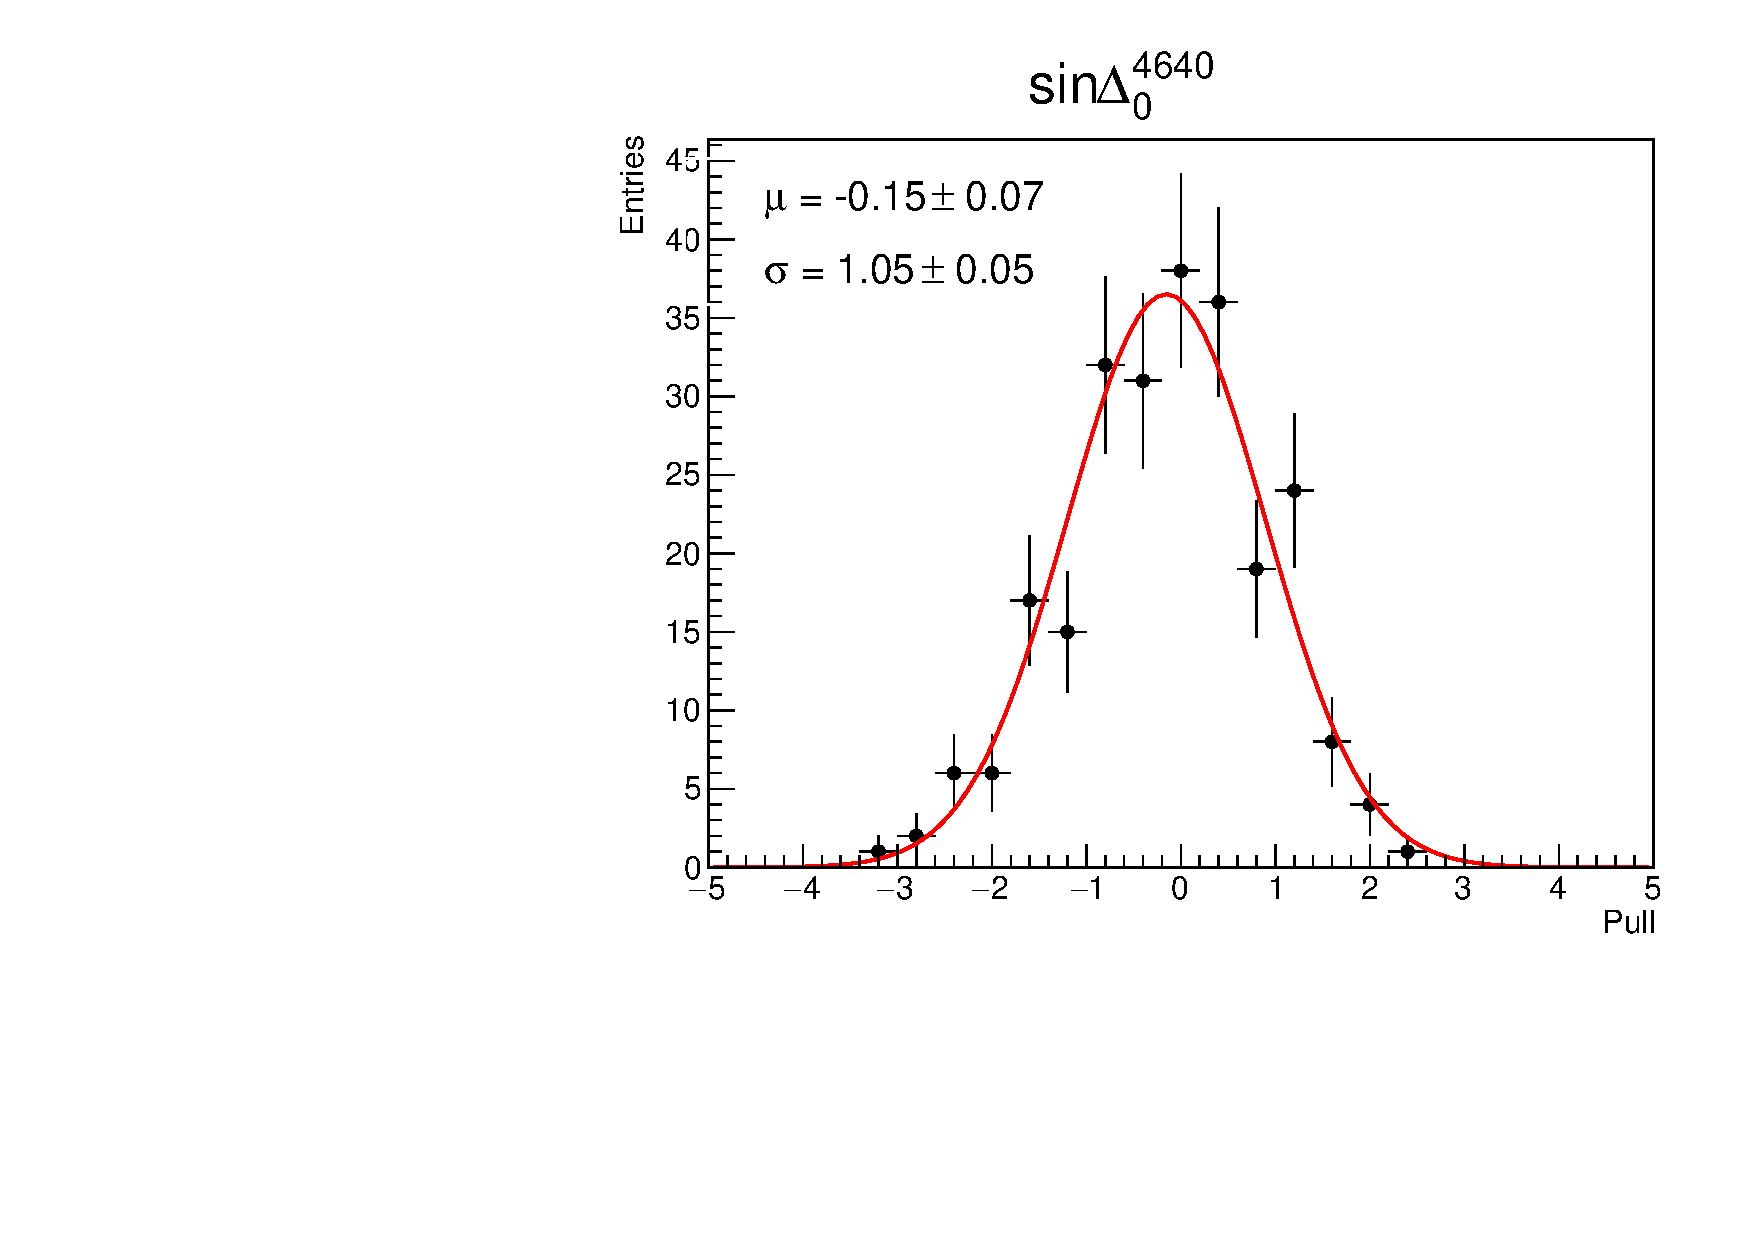
\includegraphics[width=0.24\textwidth]{figure/io_full_sim/polarization/pull_polarization_delta0_4640.pdf}
    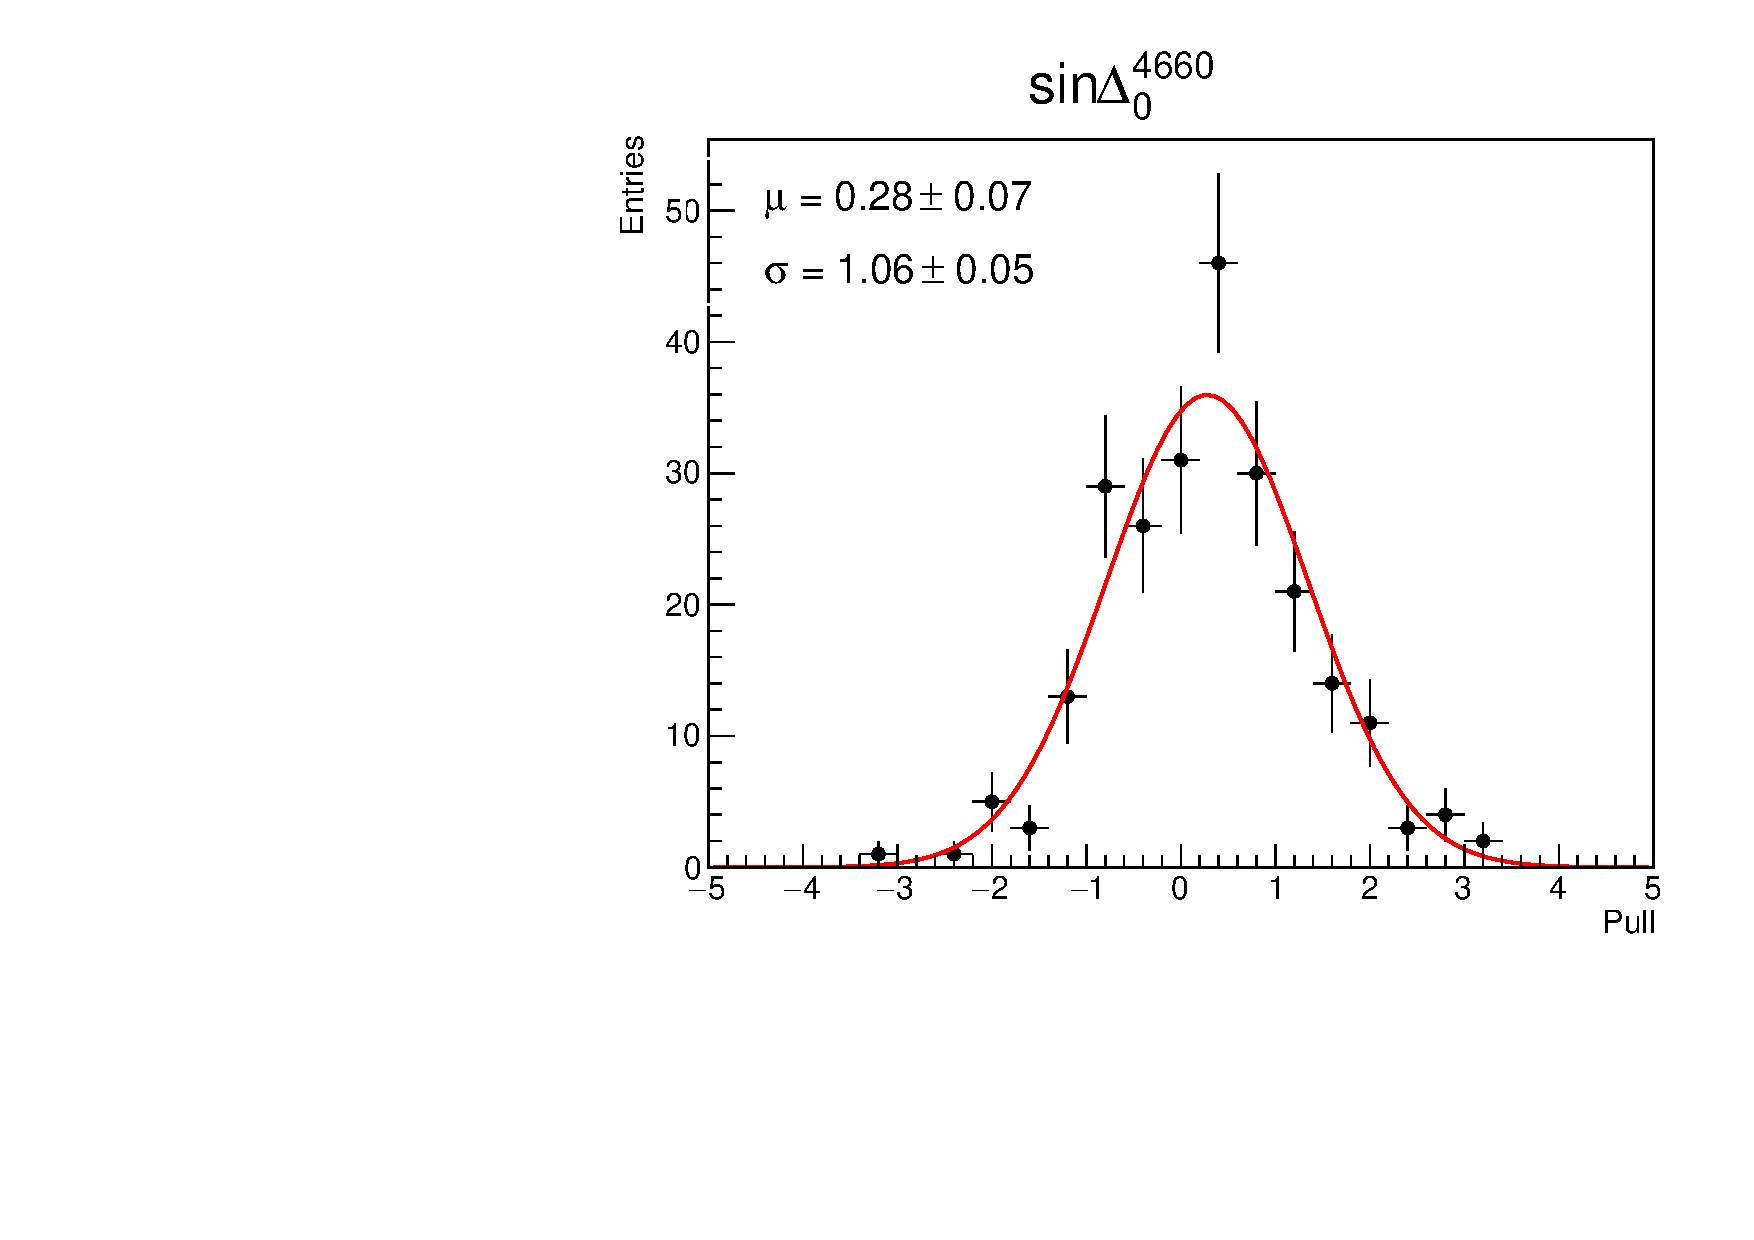
\includegraphics[width=0.24\textwidth]{figure/io_full_sim/polarization/pull_polarization_delta0_4660.pdf}
    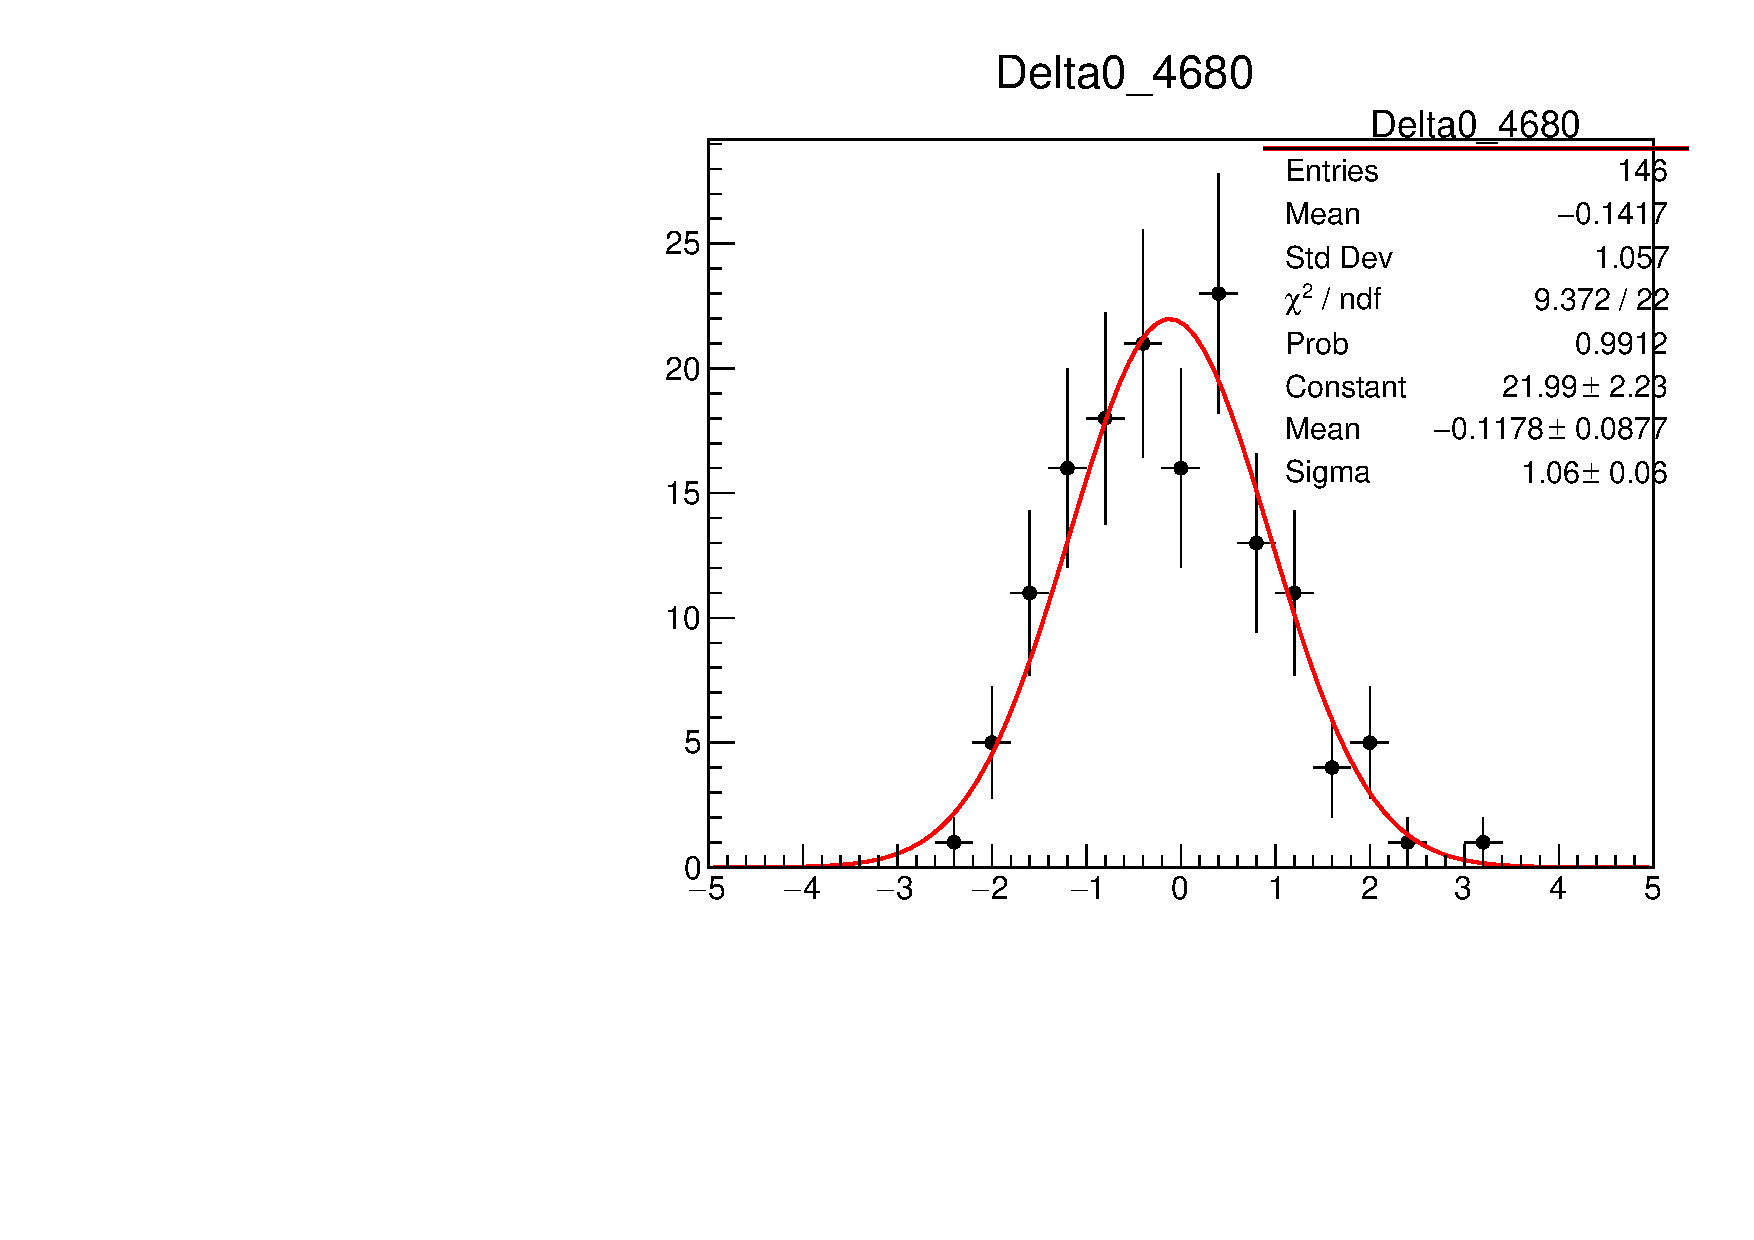
\includegraphics[width=0.24\textwidth]{figure/io_full_sim/polarization/pull_polarization_delta0_4680.pdf}
    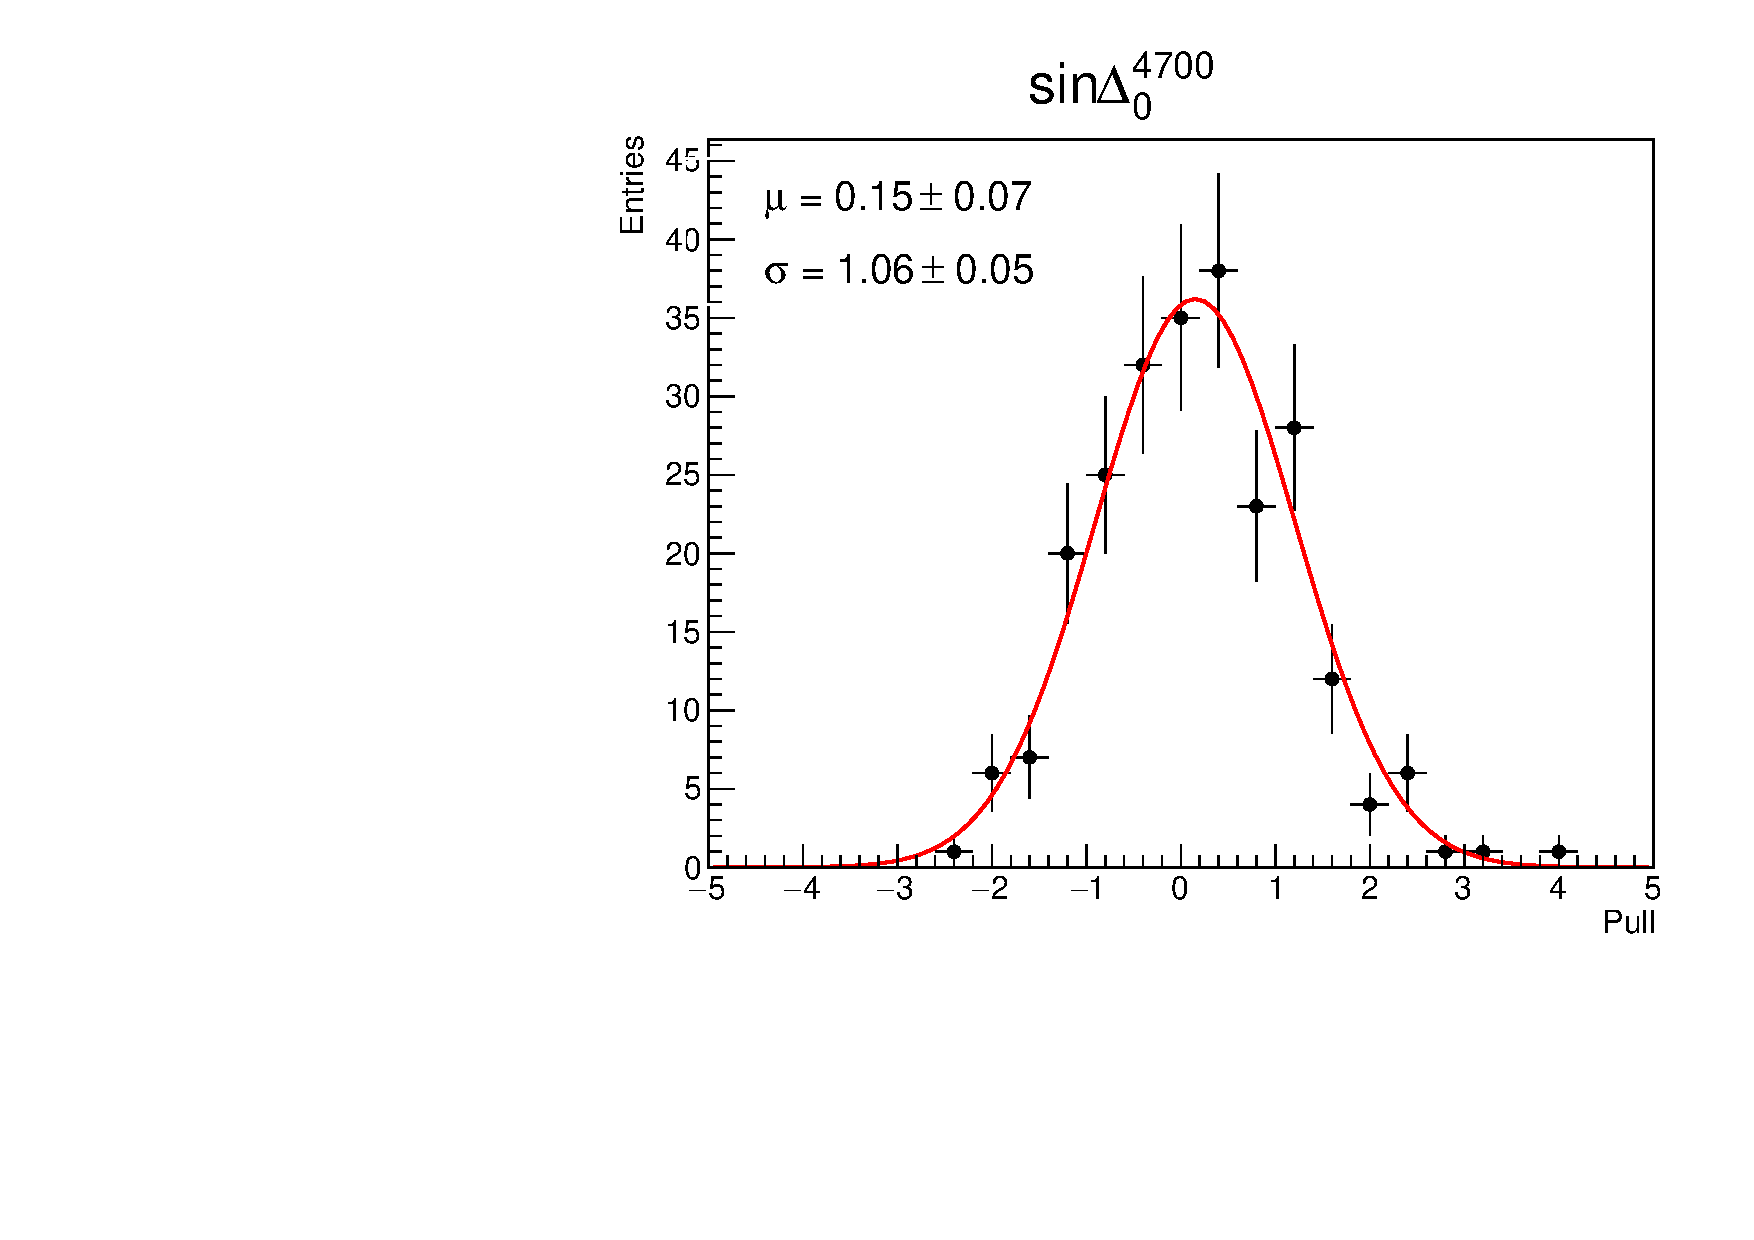
\includegraphics[width=0.24\textwidth]{figure/io_full_sim/polarization/pull_polarization_delta0_4700.pdf}
    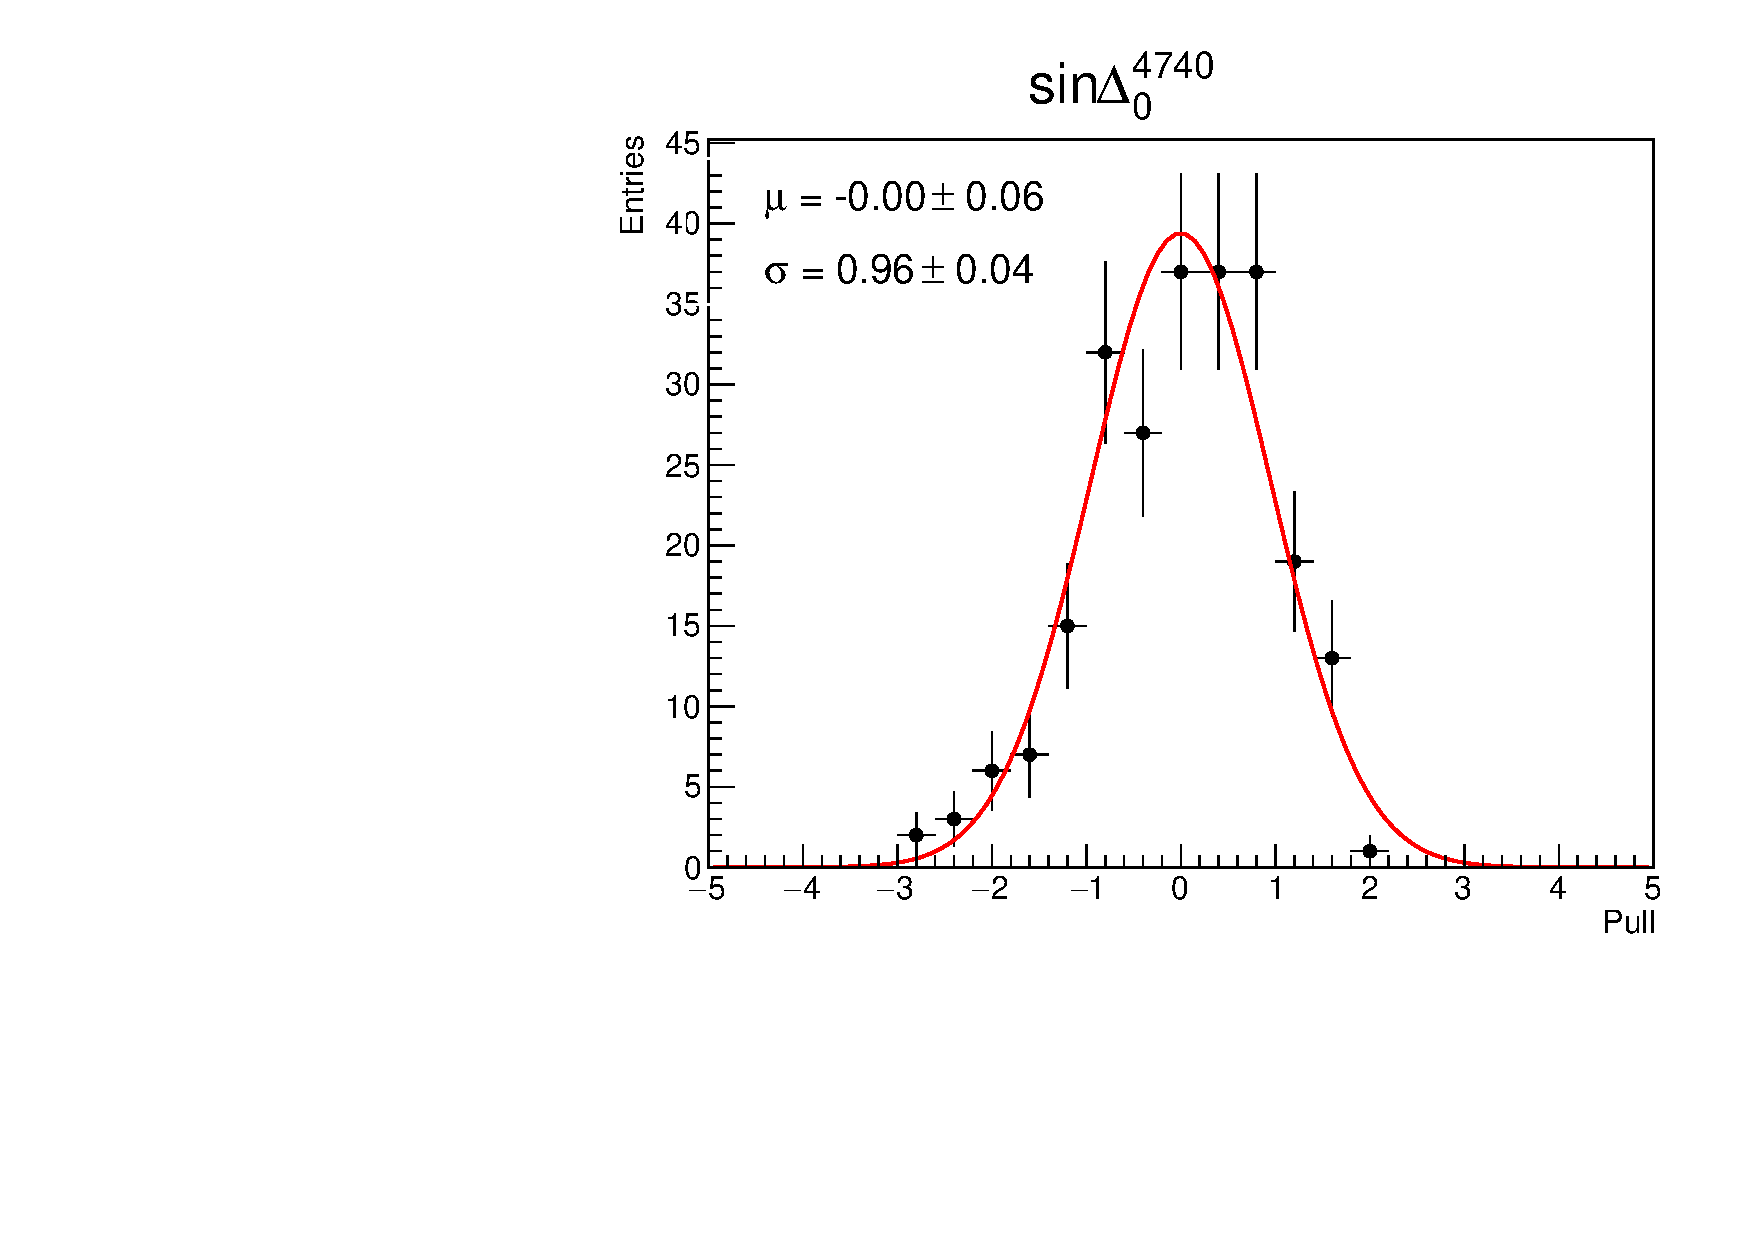
\includegraphics[width=0.24\textwidth]{figure/io_full_sim/polarization/pull_polarization_delta0_4740.pdf}
    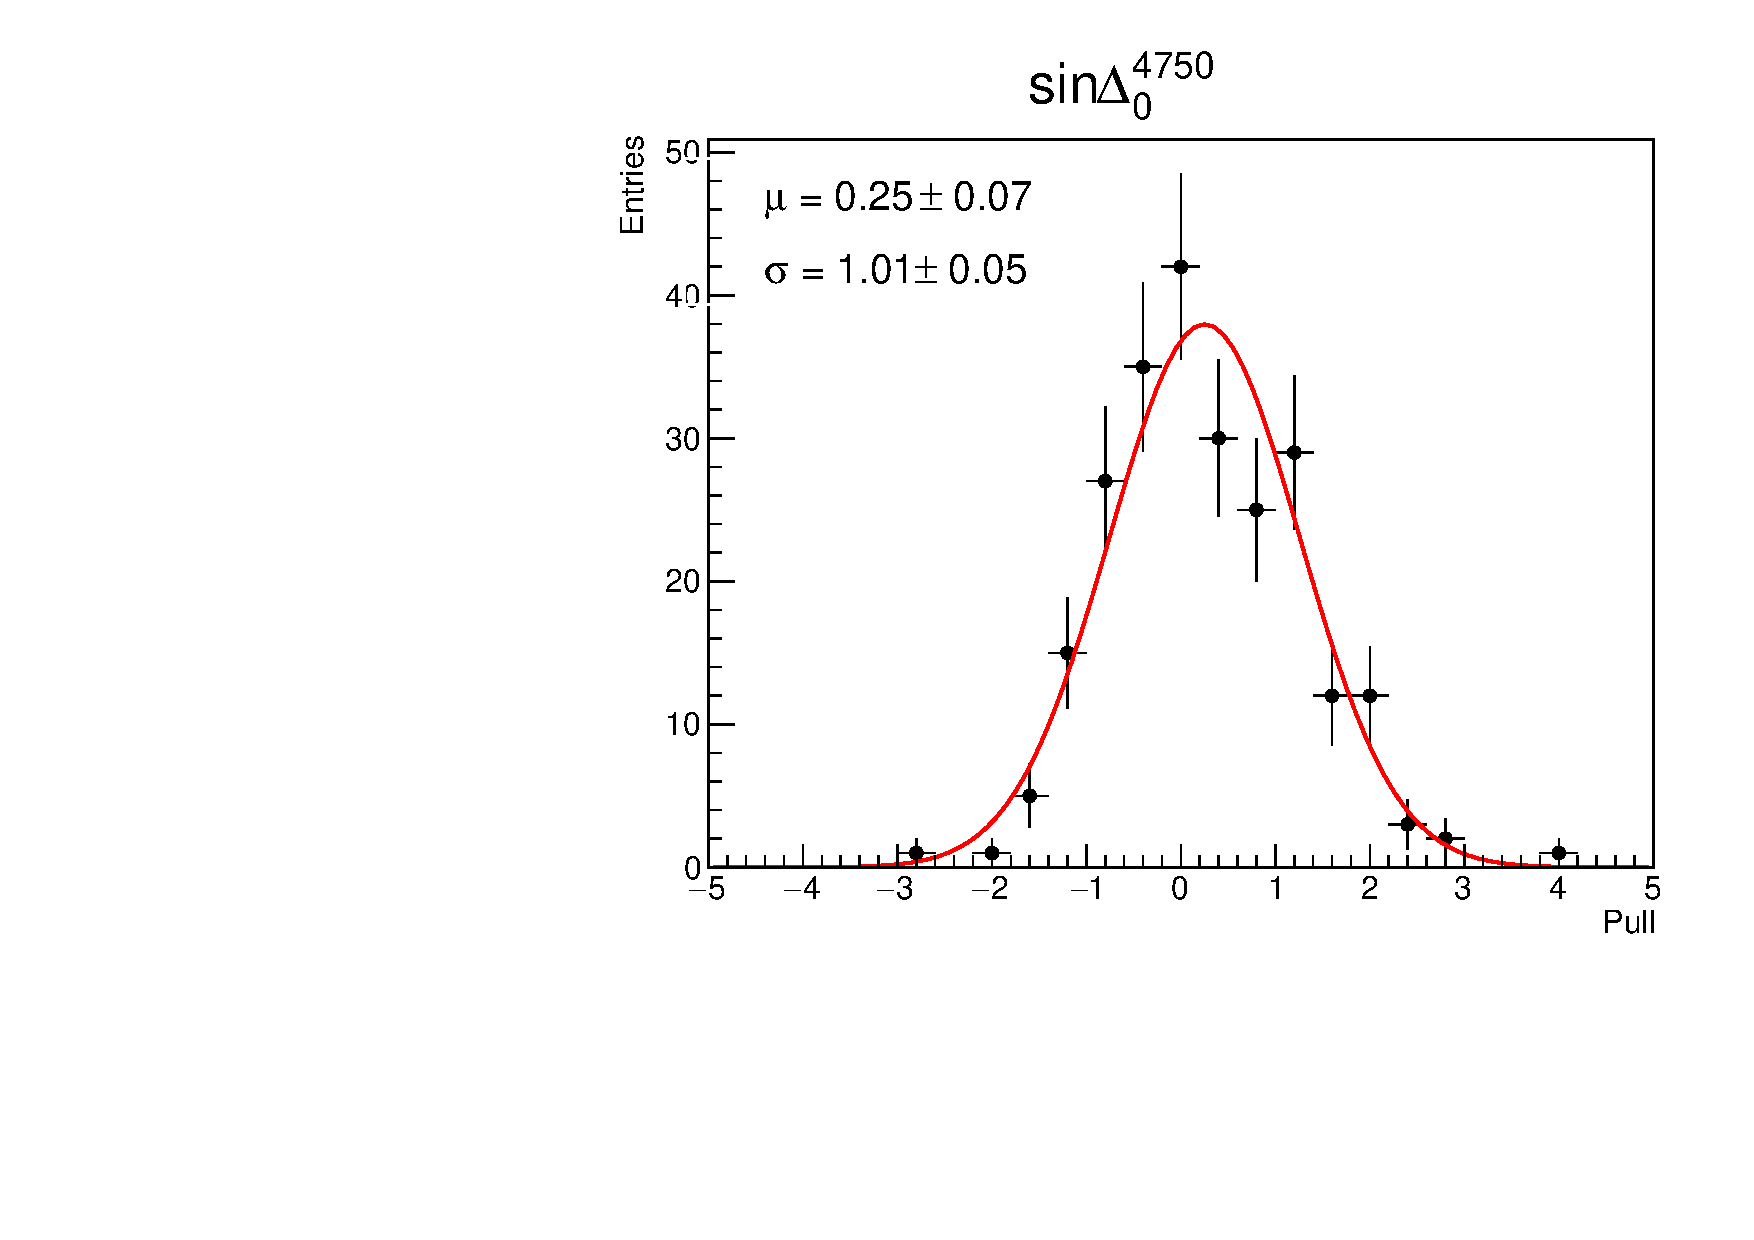
\includegraphics[width=0.24\textwidth]{figure/io_full_sim/polarization/pull_polarization_delta0_4750.pdf}
    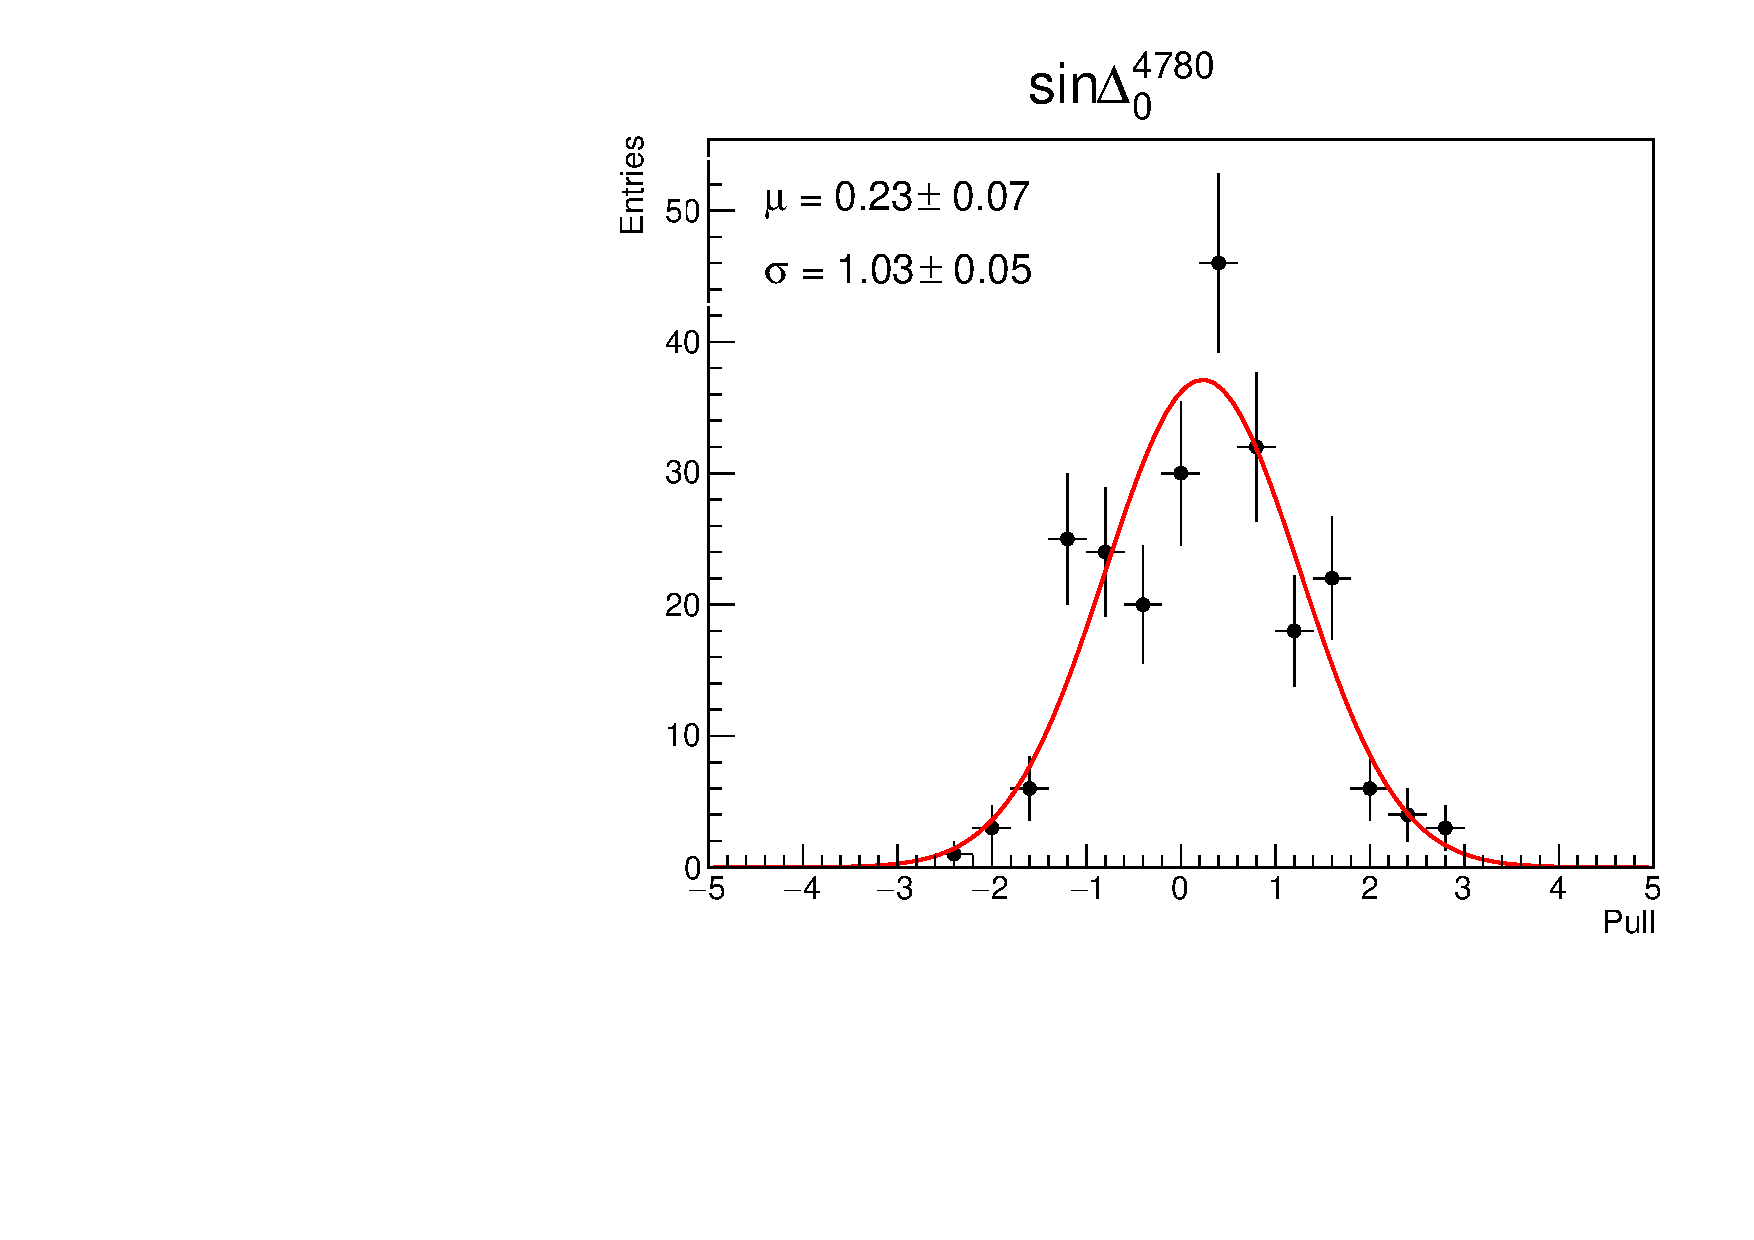
\includegraphics[width=0.24\textwidth]{figure/io_full_sim/polarization/pull_polarization_delta0_4780.pdf}
    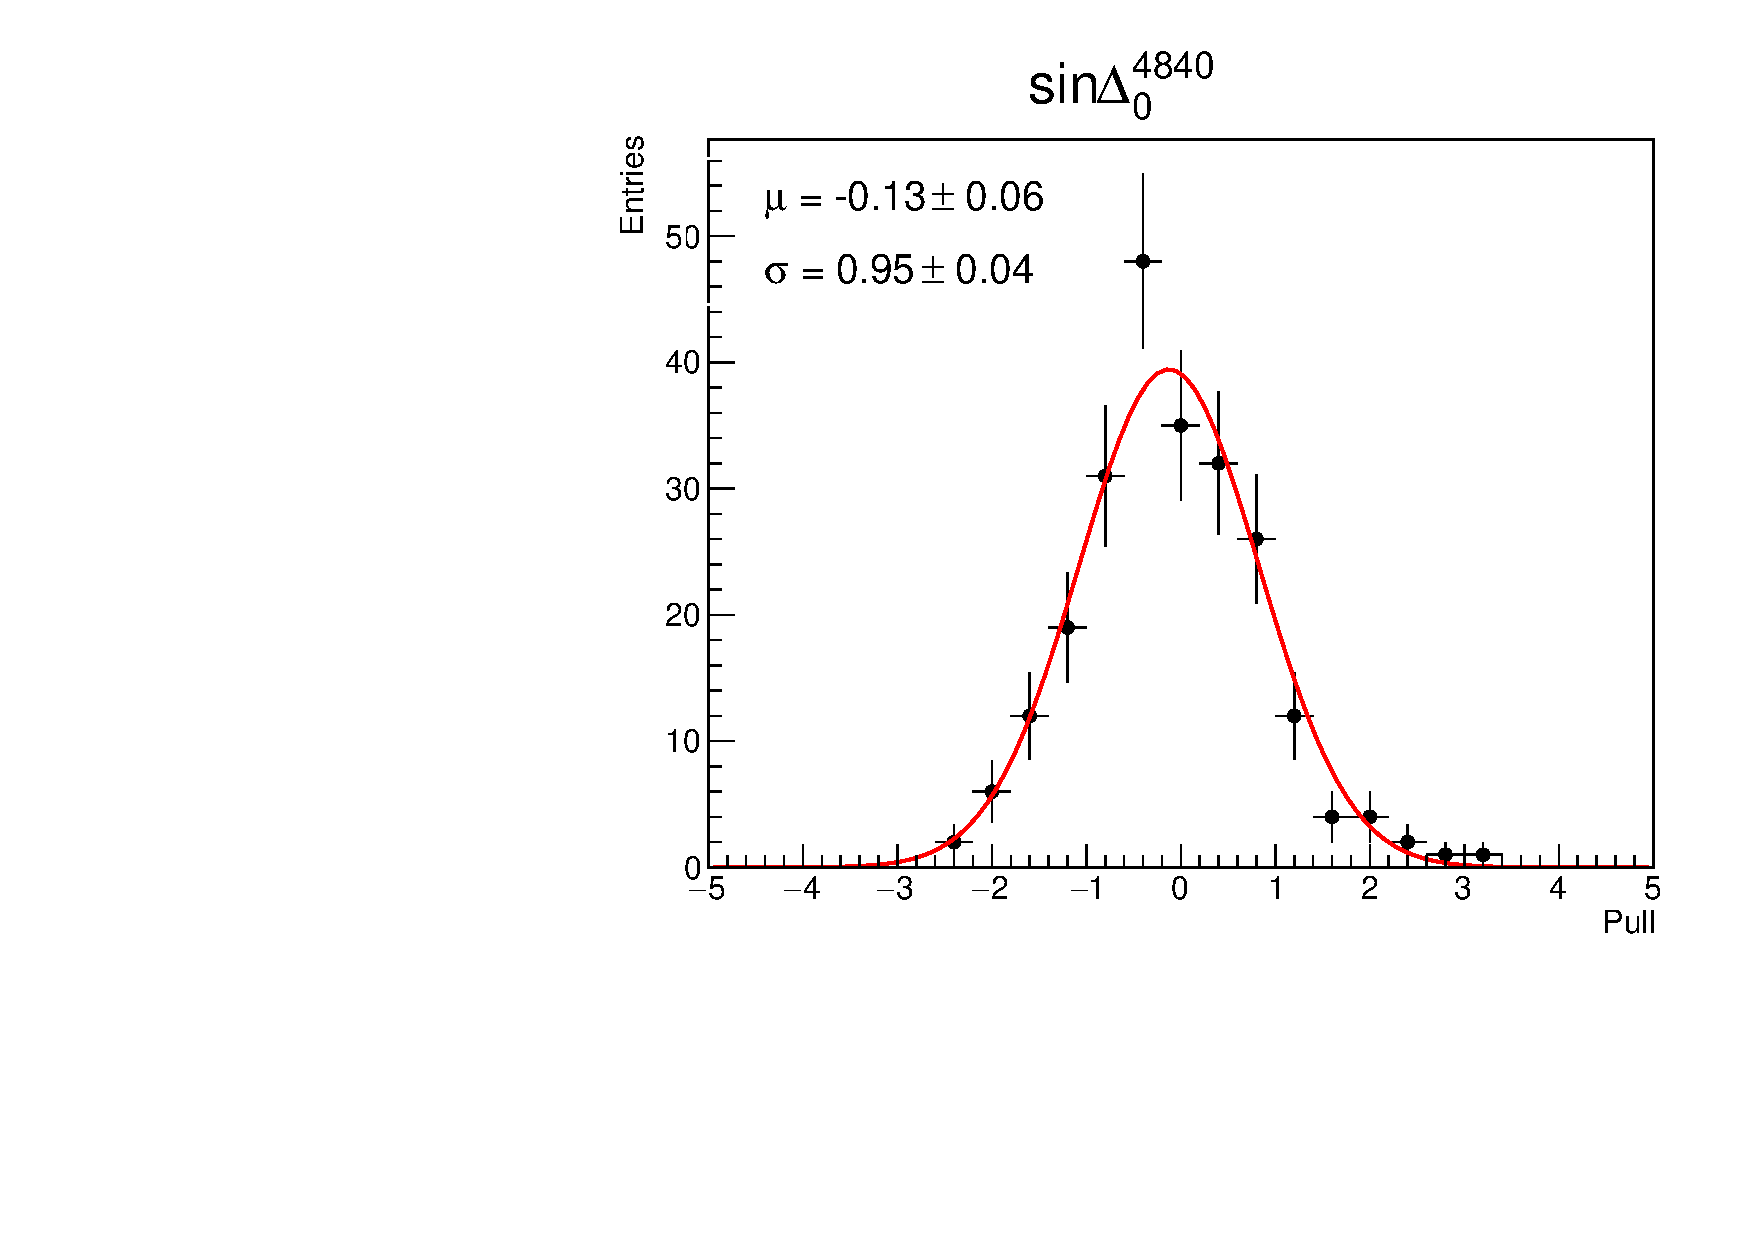
\includegraphics[width=0.24\textwidth]{figure/io_full_sim/polarization/pull_polarization_delta0_4840.pdf}
    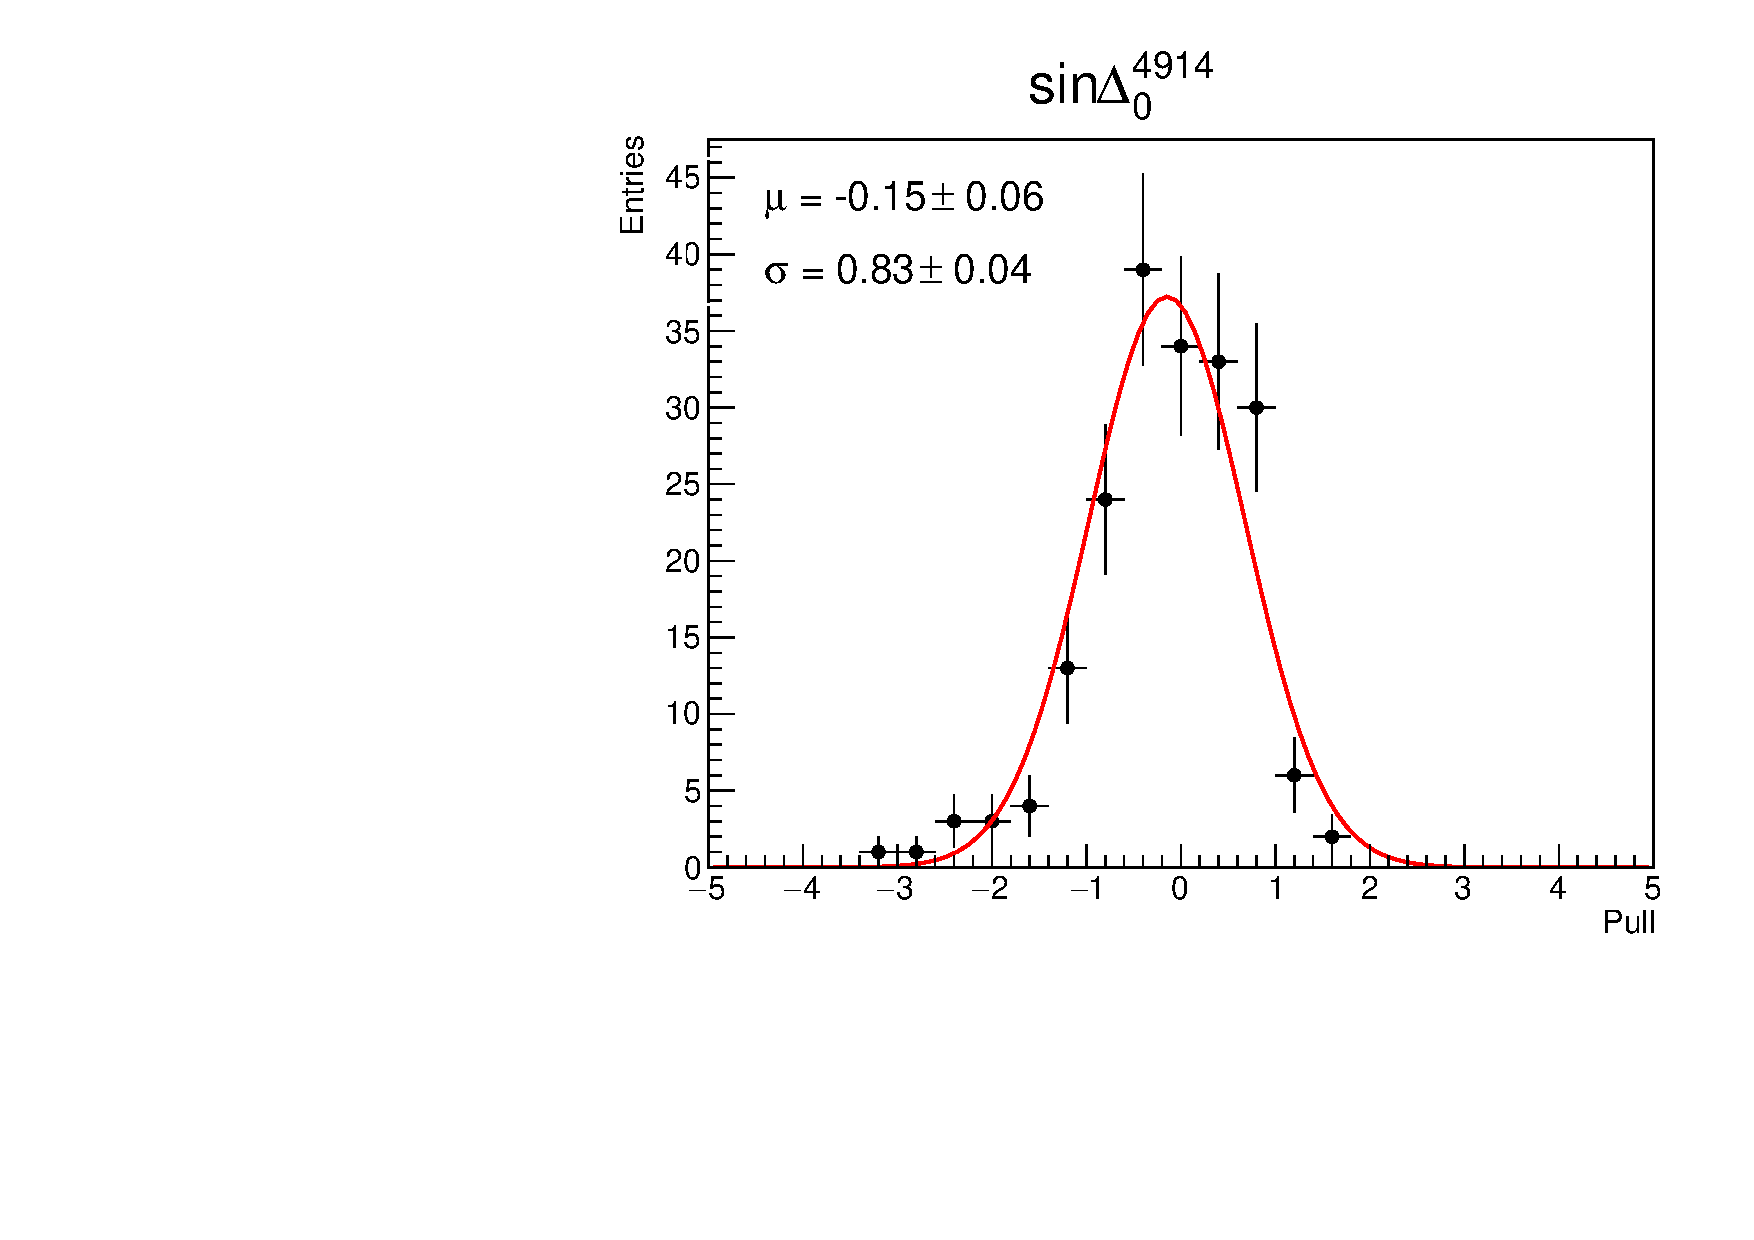
\includegraphics[width=0.24\textwidth]{figure/io_full_sim/polarization/pull_polarization_delta0_4914.pdf}
    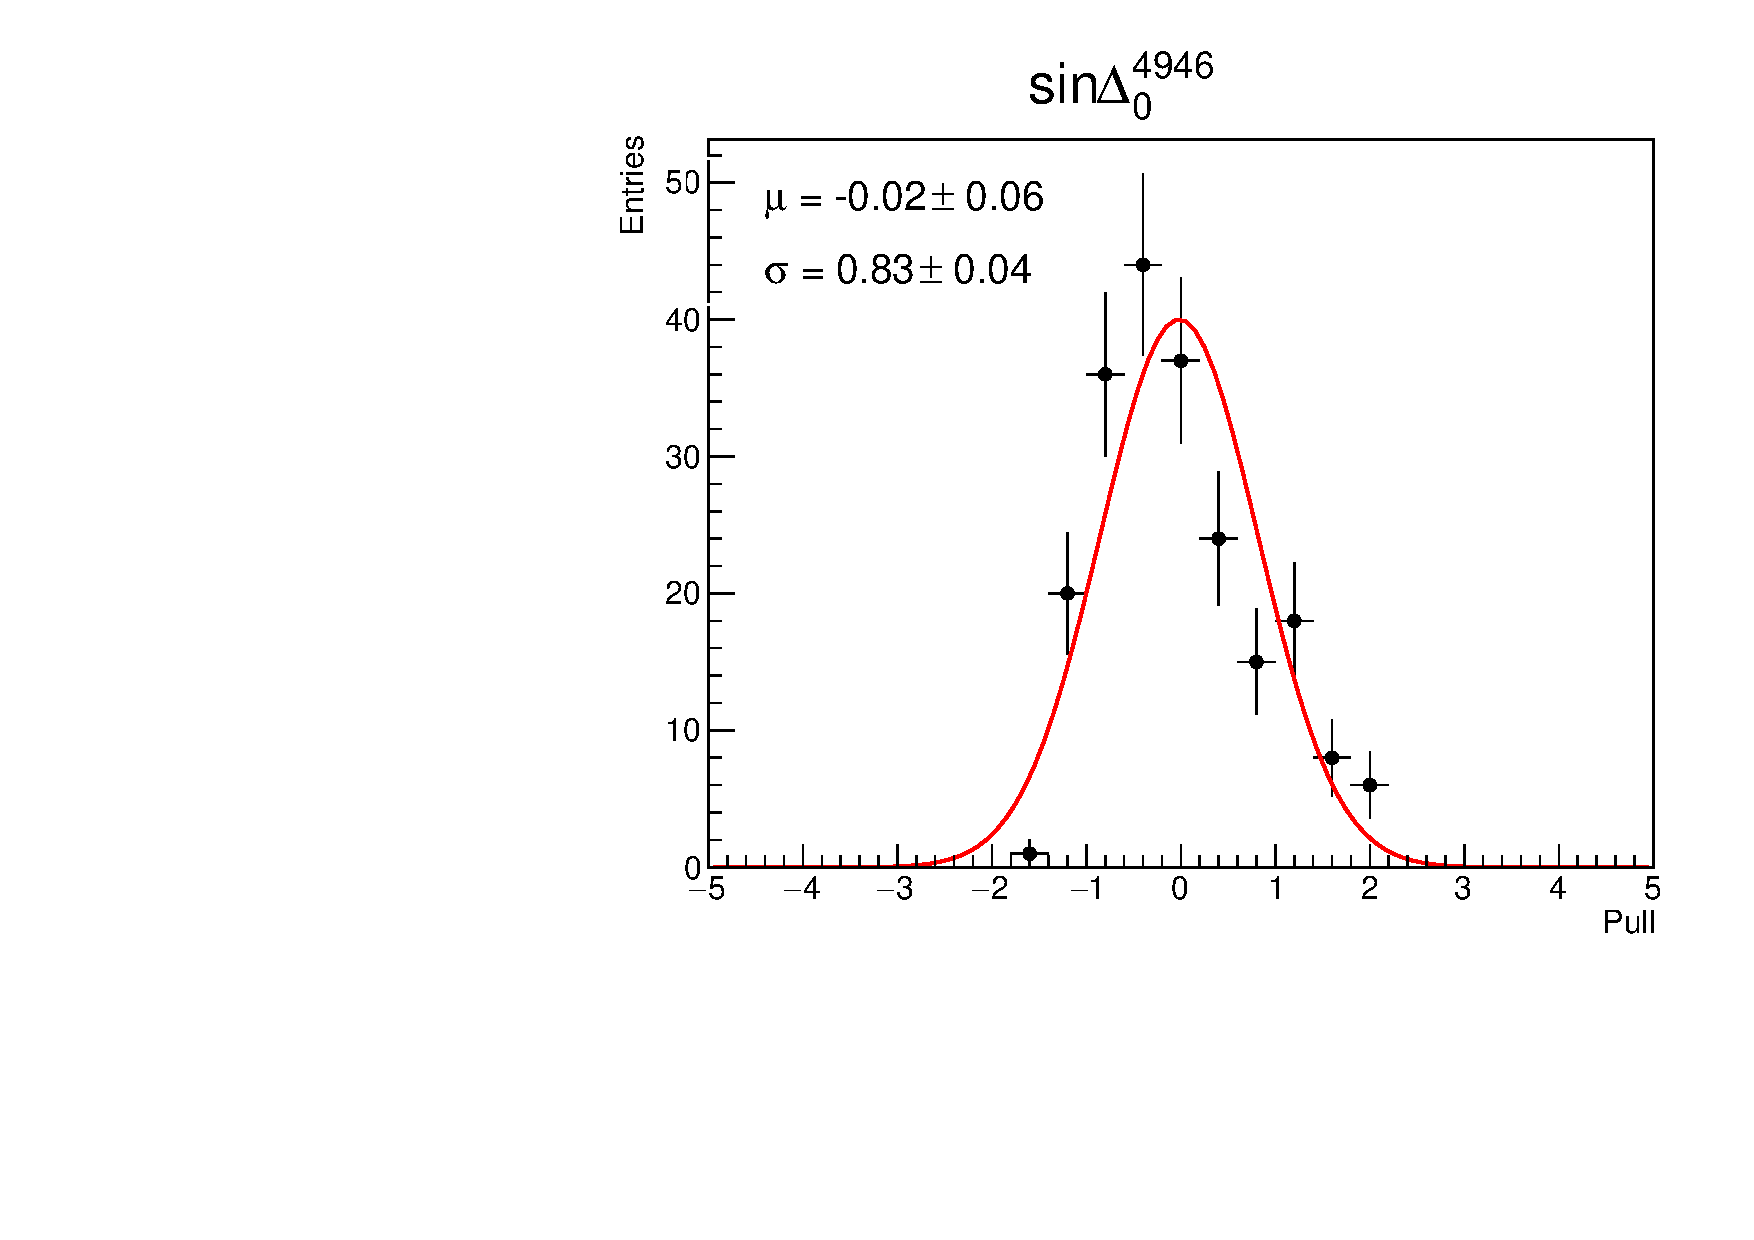
\includegraphics[width=0.24\textwidth]{figure/io_full_sim/polarization/pull_polarization_delta0_4946.pdf}
    \caption{Pull distributions of $\sin\Delta_0$ for each energy point.}
\label{fig:io_wo_bkg_pull_delta0}
\end{figure}

\begin{figure}[h]\centering
    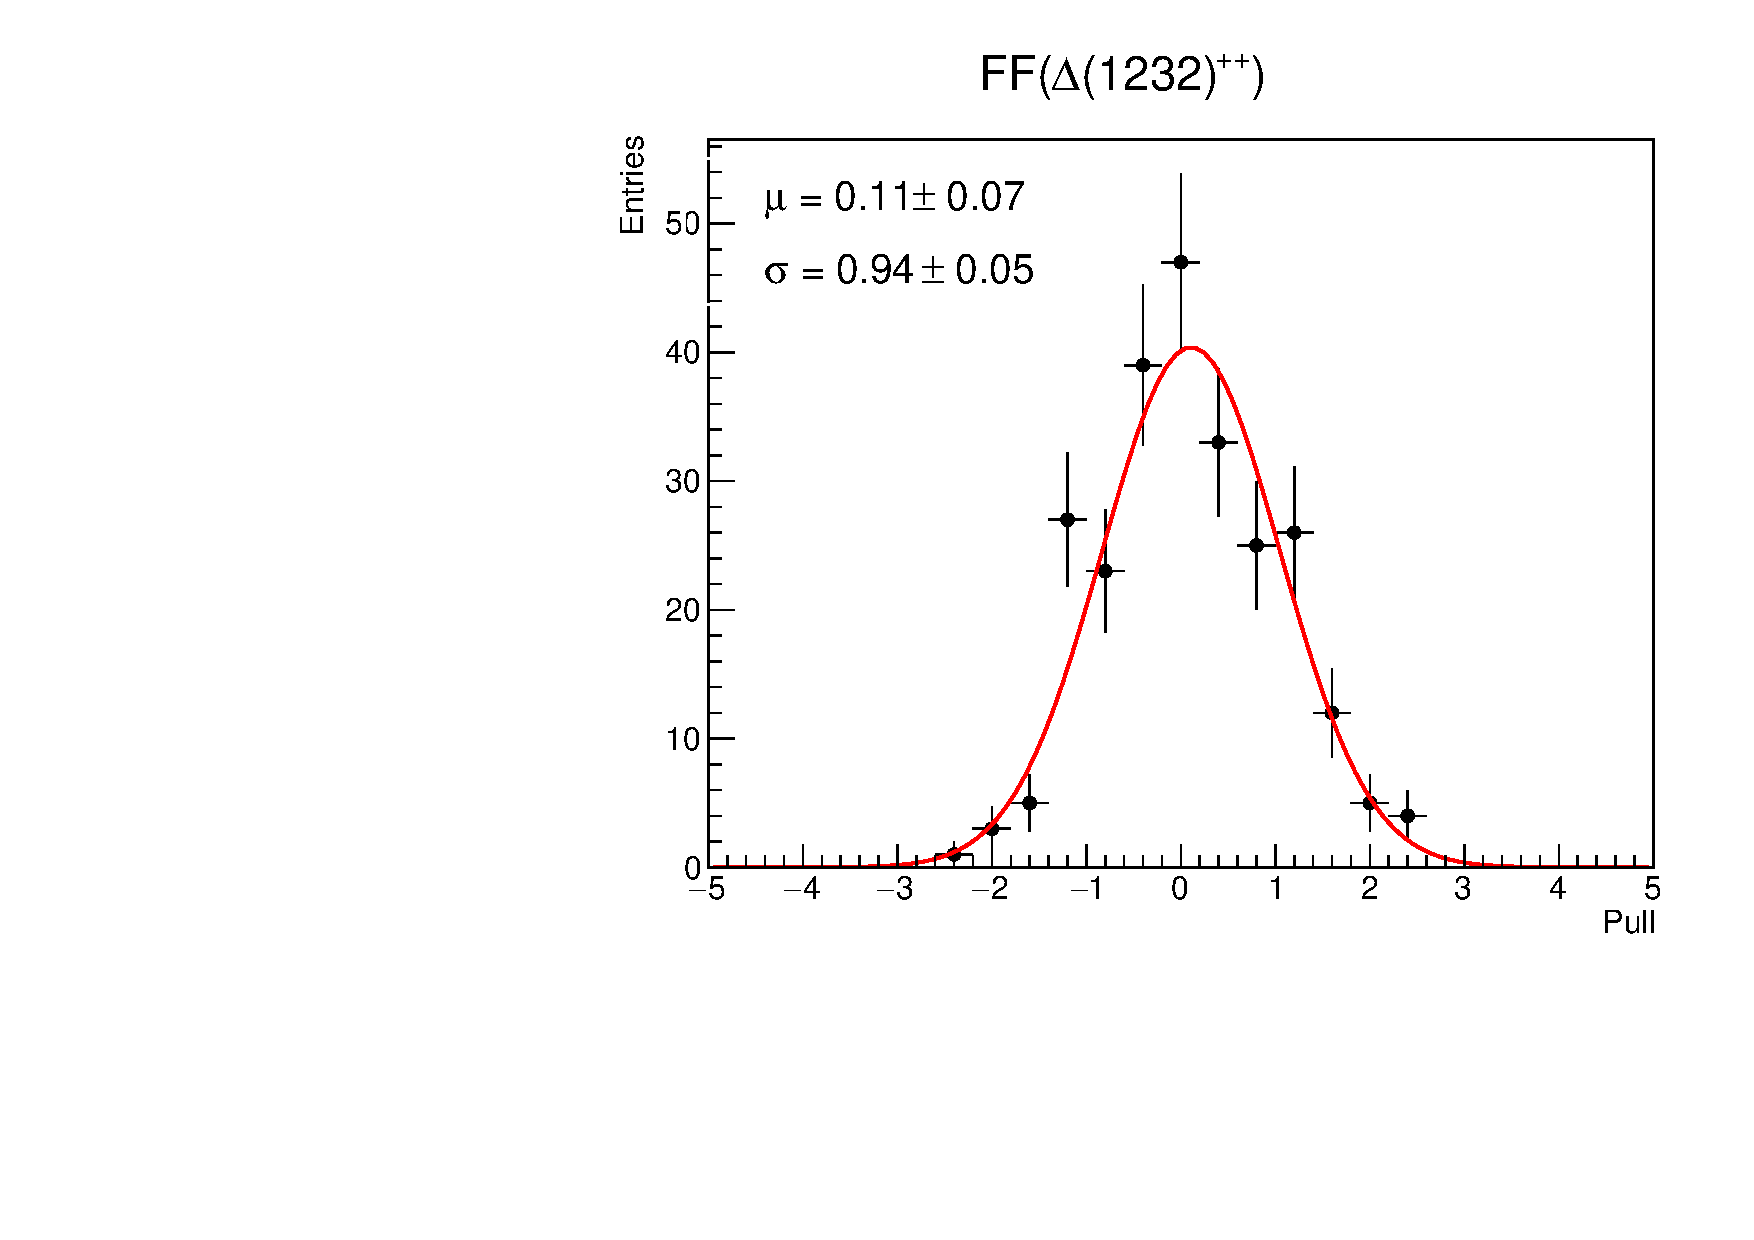
\includegraphics[width=0.24\textwidth]{figure/io_full_sim/fitfrac/pull_fitfrac_res0_comb.pdf}
    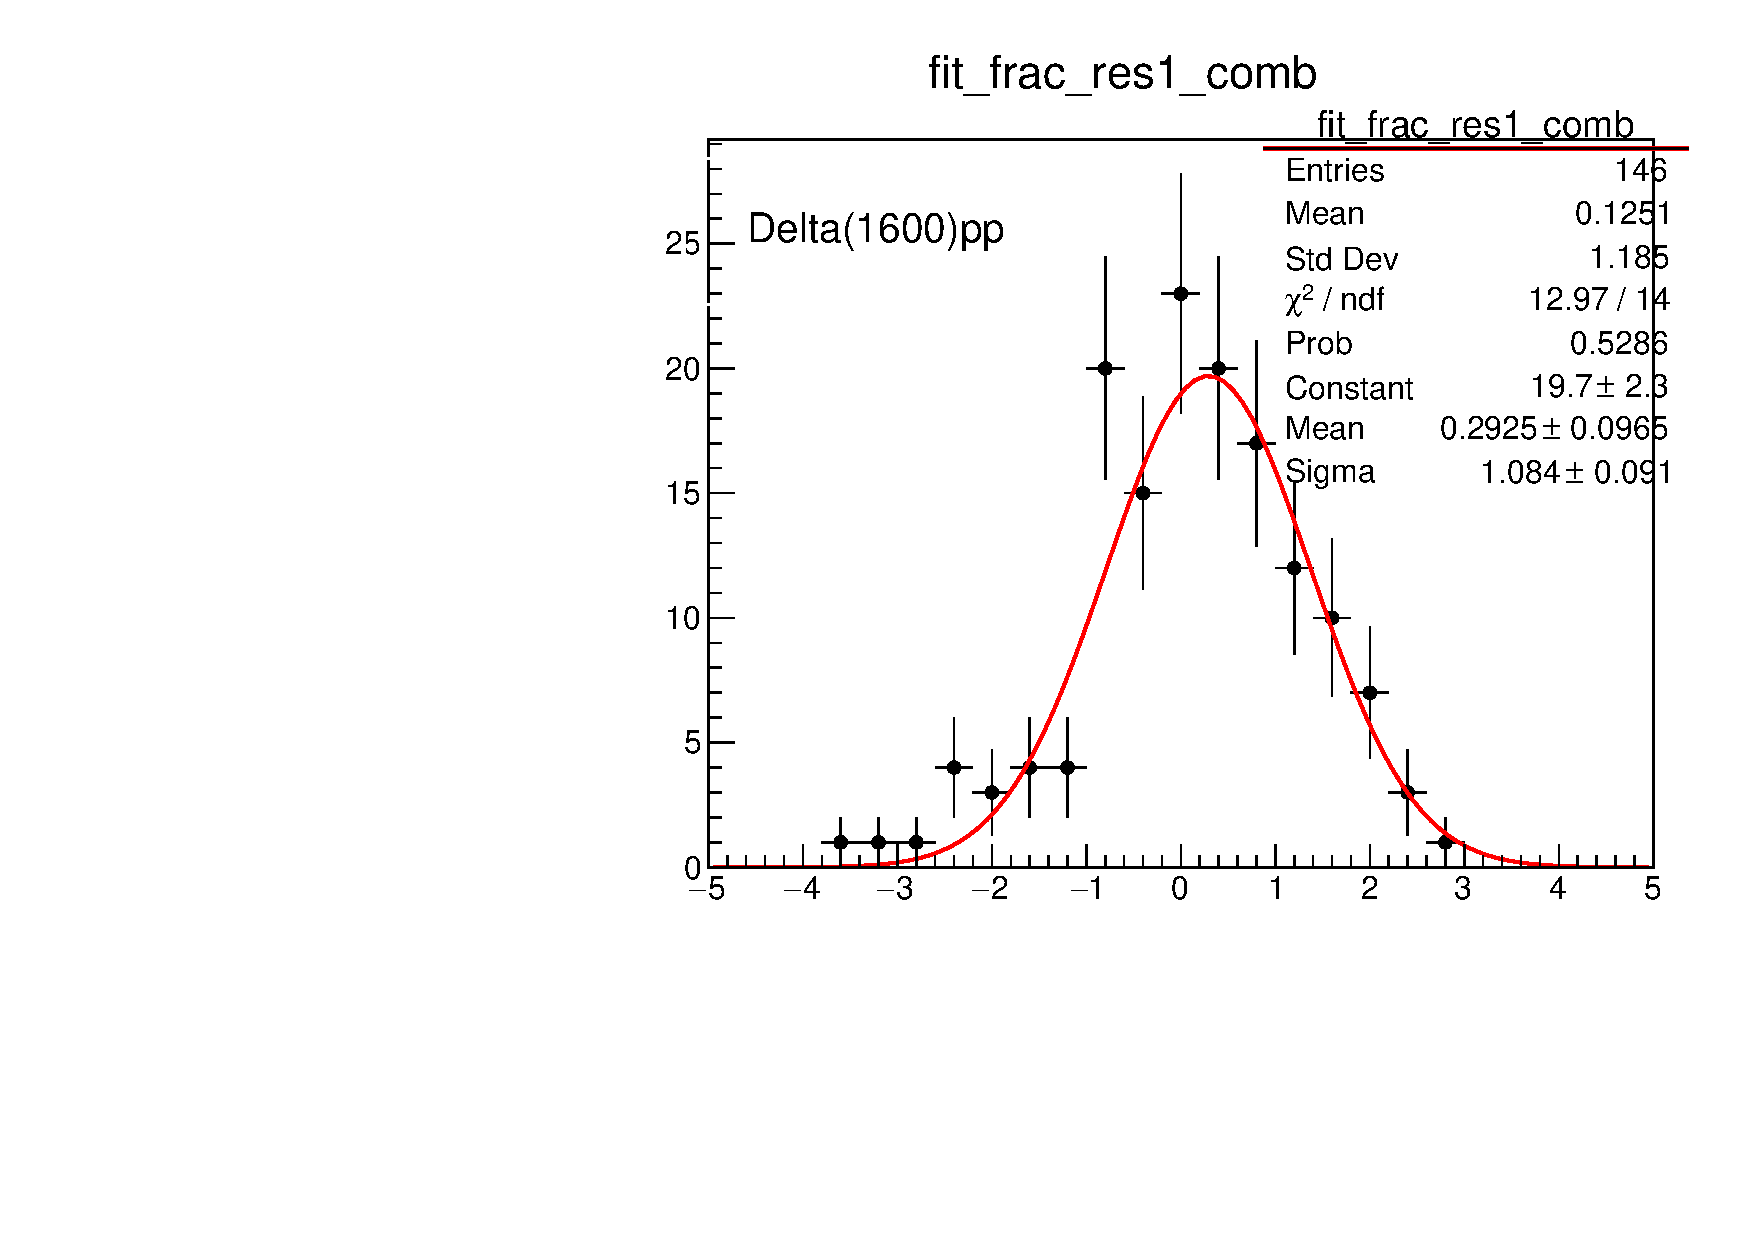
\includegraphics[width=0.24\textwidth]{figure/io_full_sim/fitfrac/pull_fitfrac_res1_comb.pdf}
    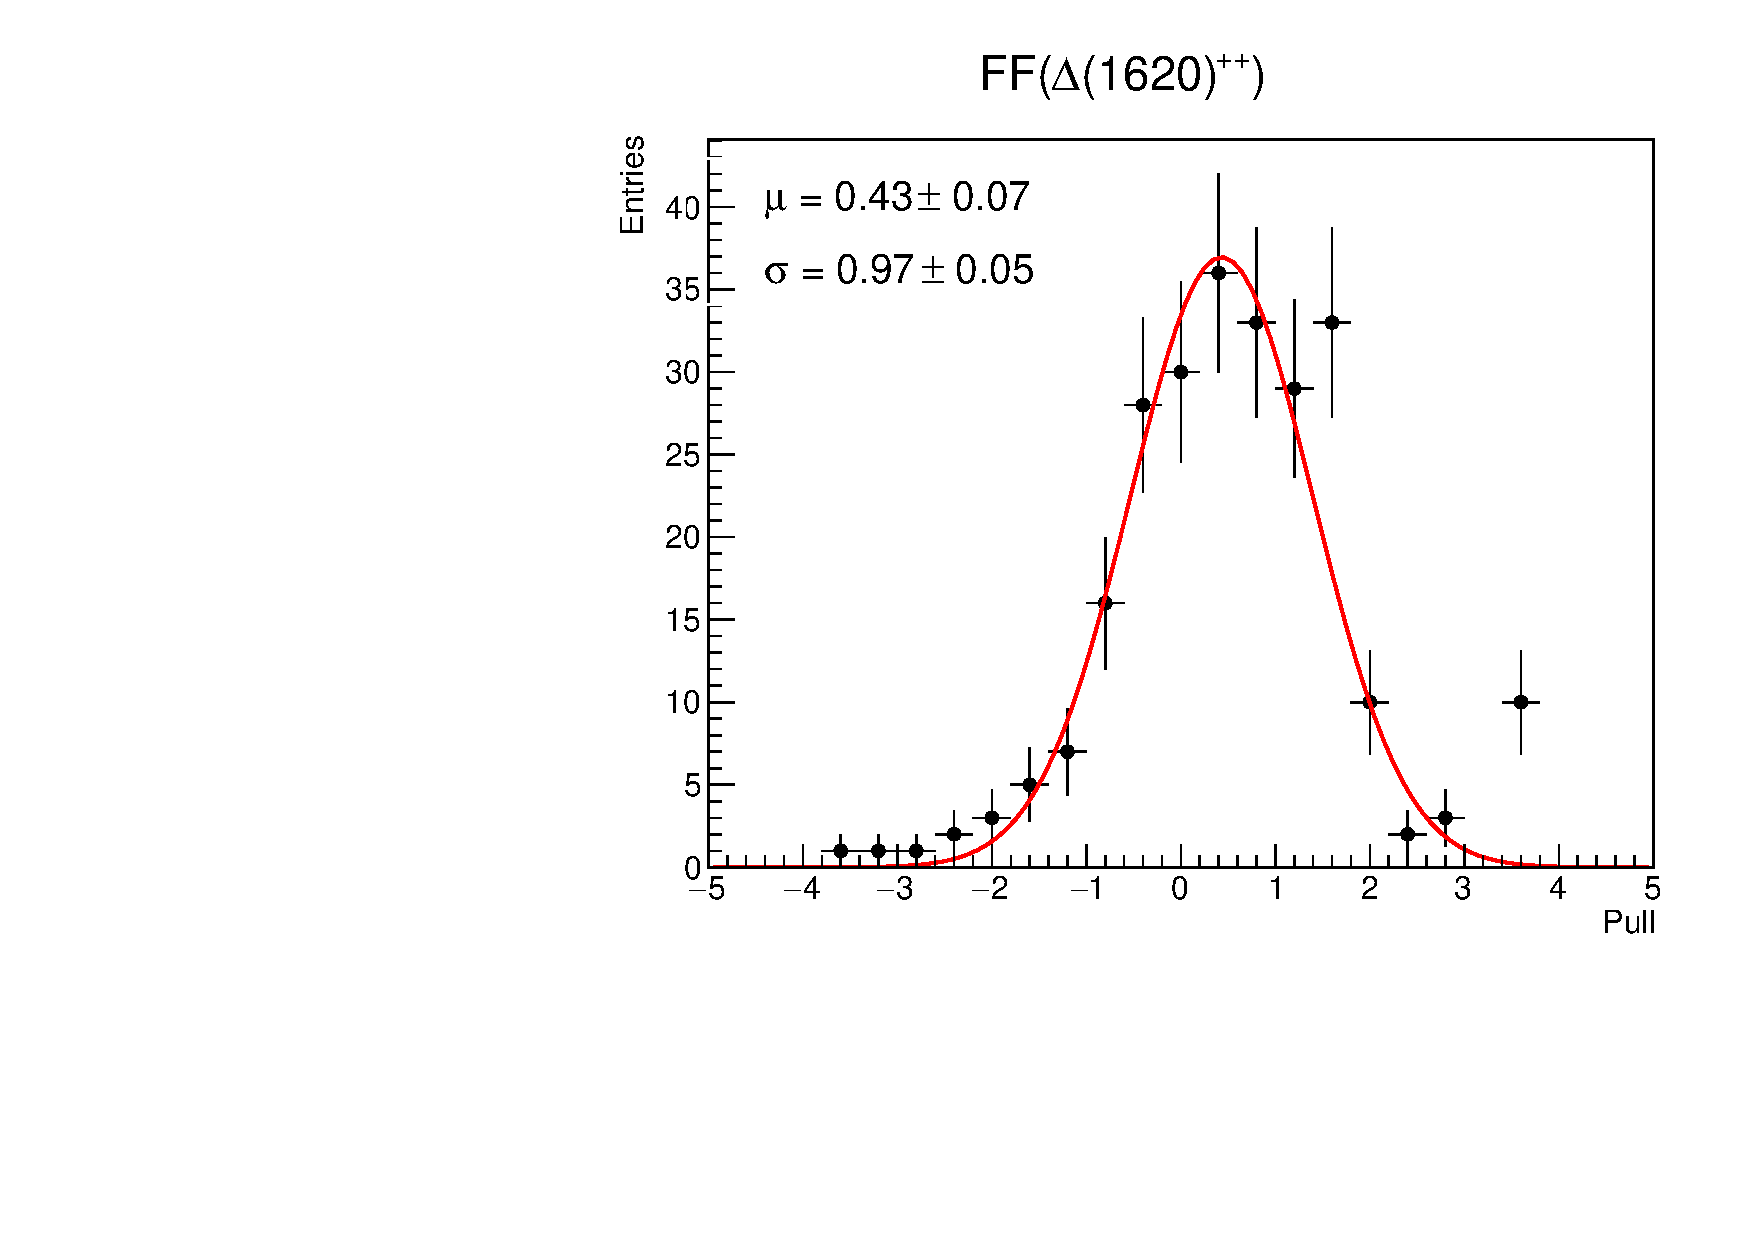
\includegraphics[width=0.24\textwidth]{figure/io_full_sim/fitfrac/pull_fitfrac_res2_comb.pdf}
    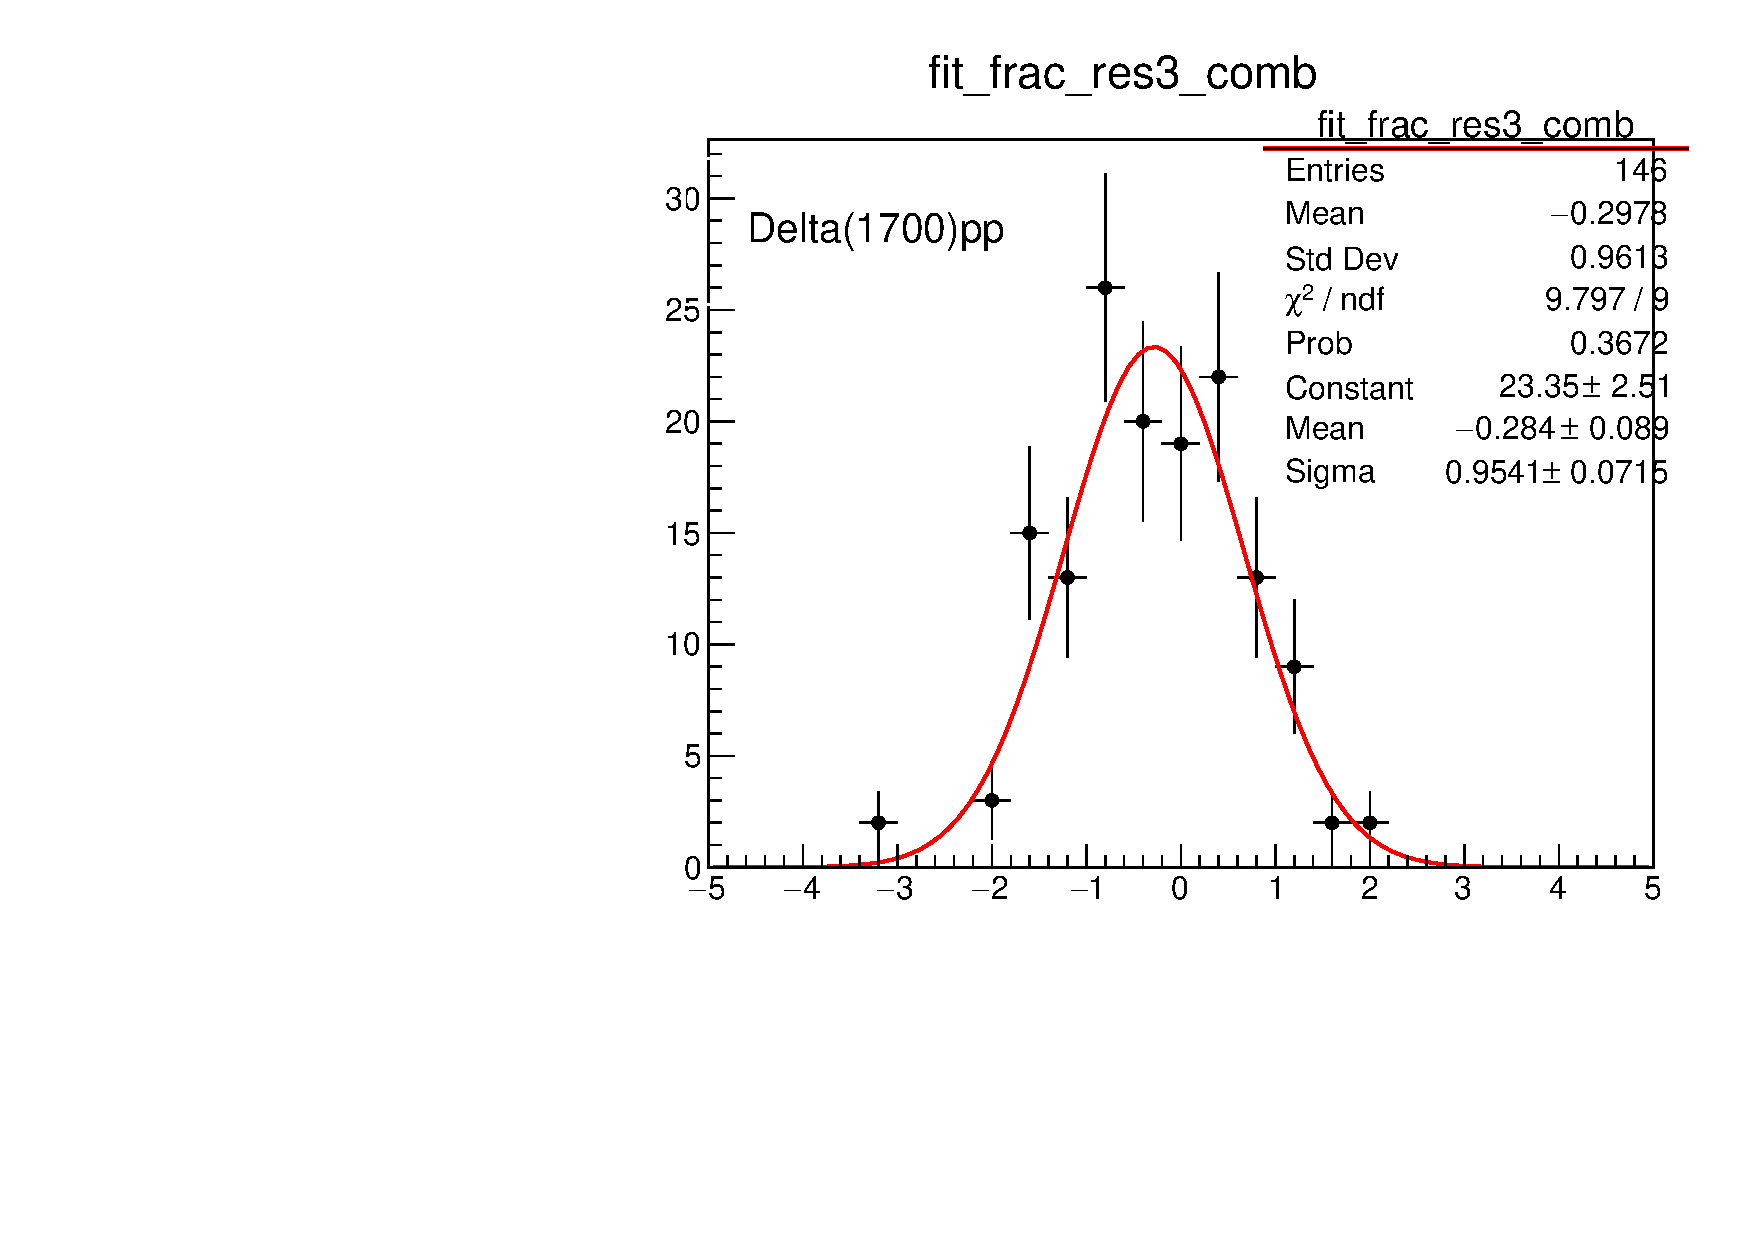
\includegraphics[width=0.24\textwidth]{figure/io_full_sim/fitfrac/pull_fitfrac_res3_comb.pdf}
    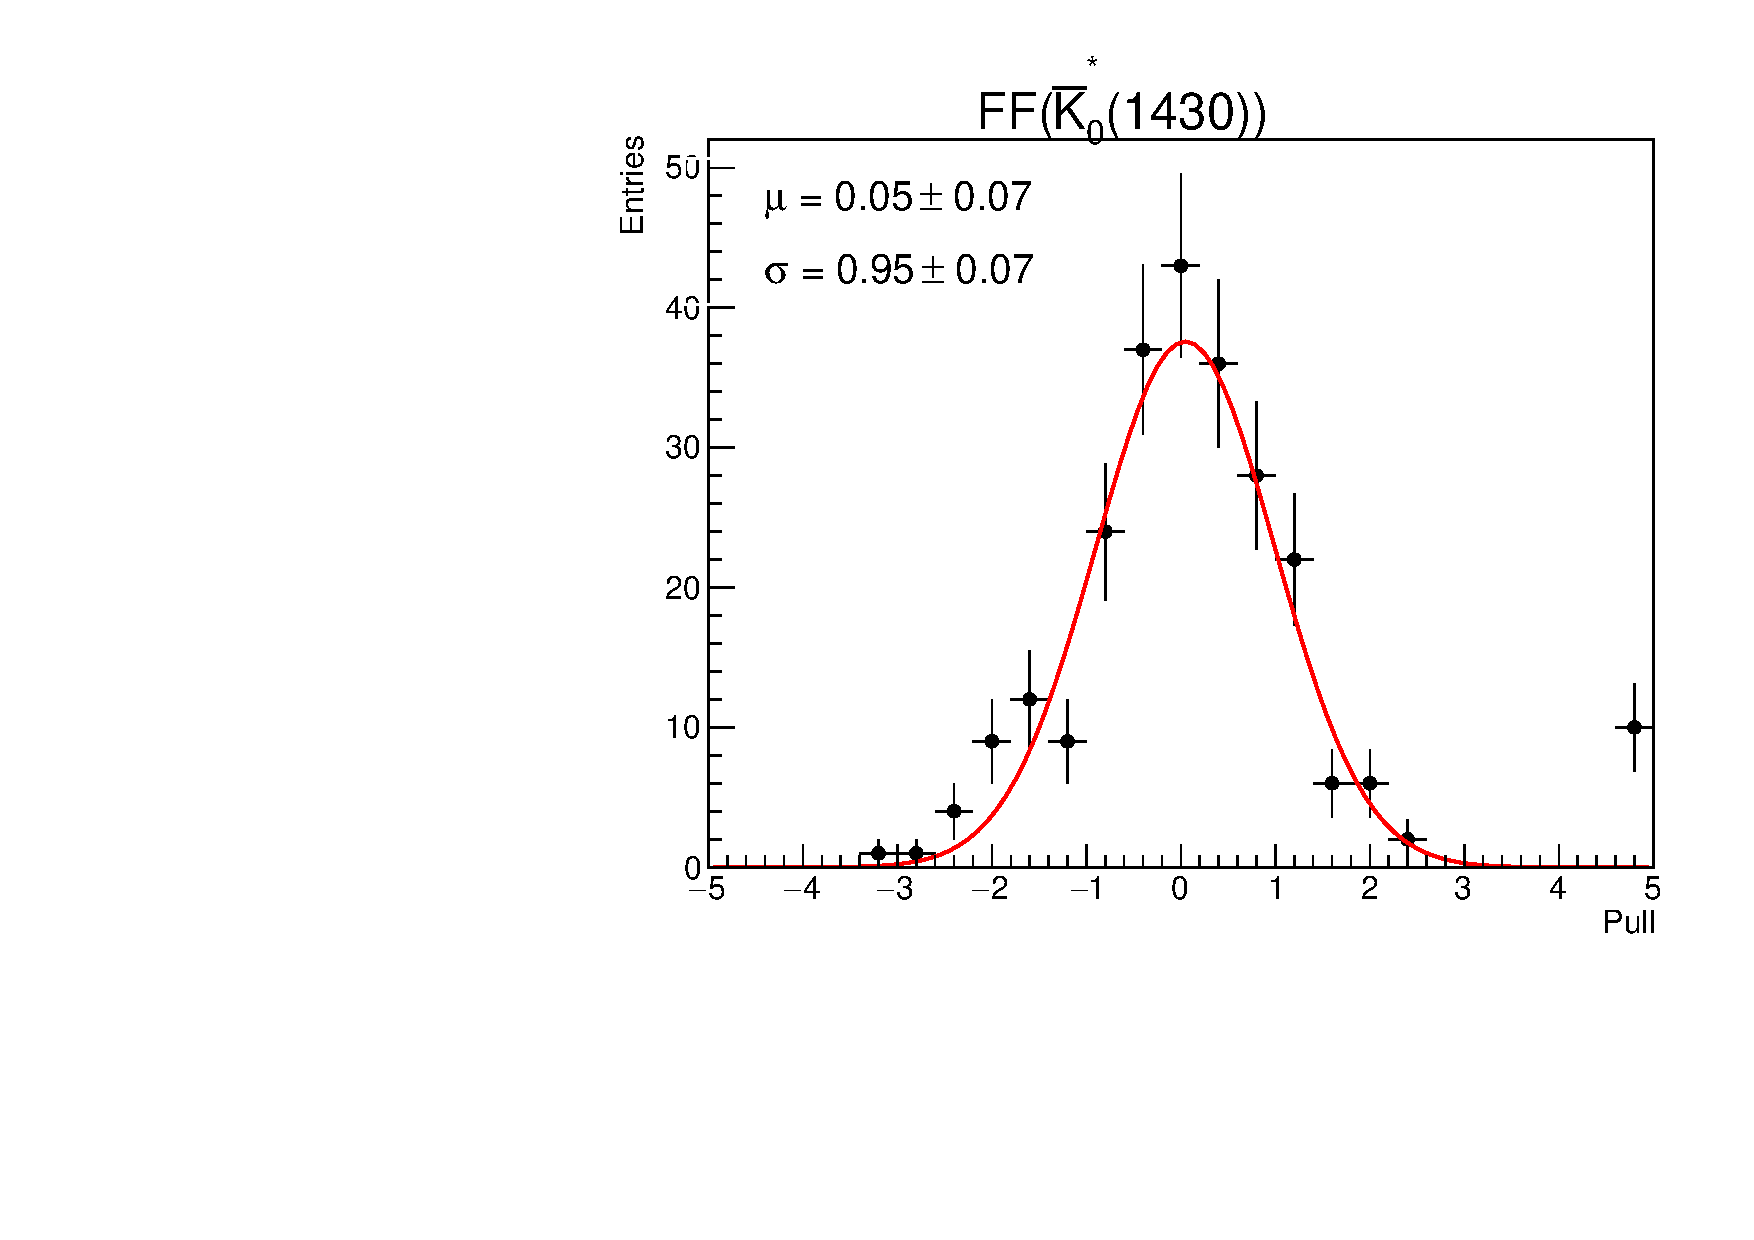
\includegraphics[width=0.24\textwidth]{figure/io_full_sim/fitfrac/pull_fitfrac_res4_comb.pdf}
    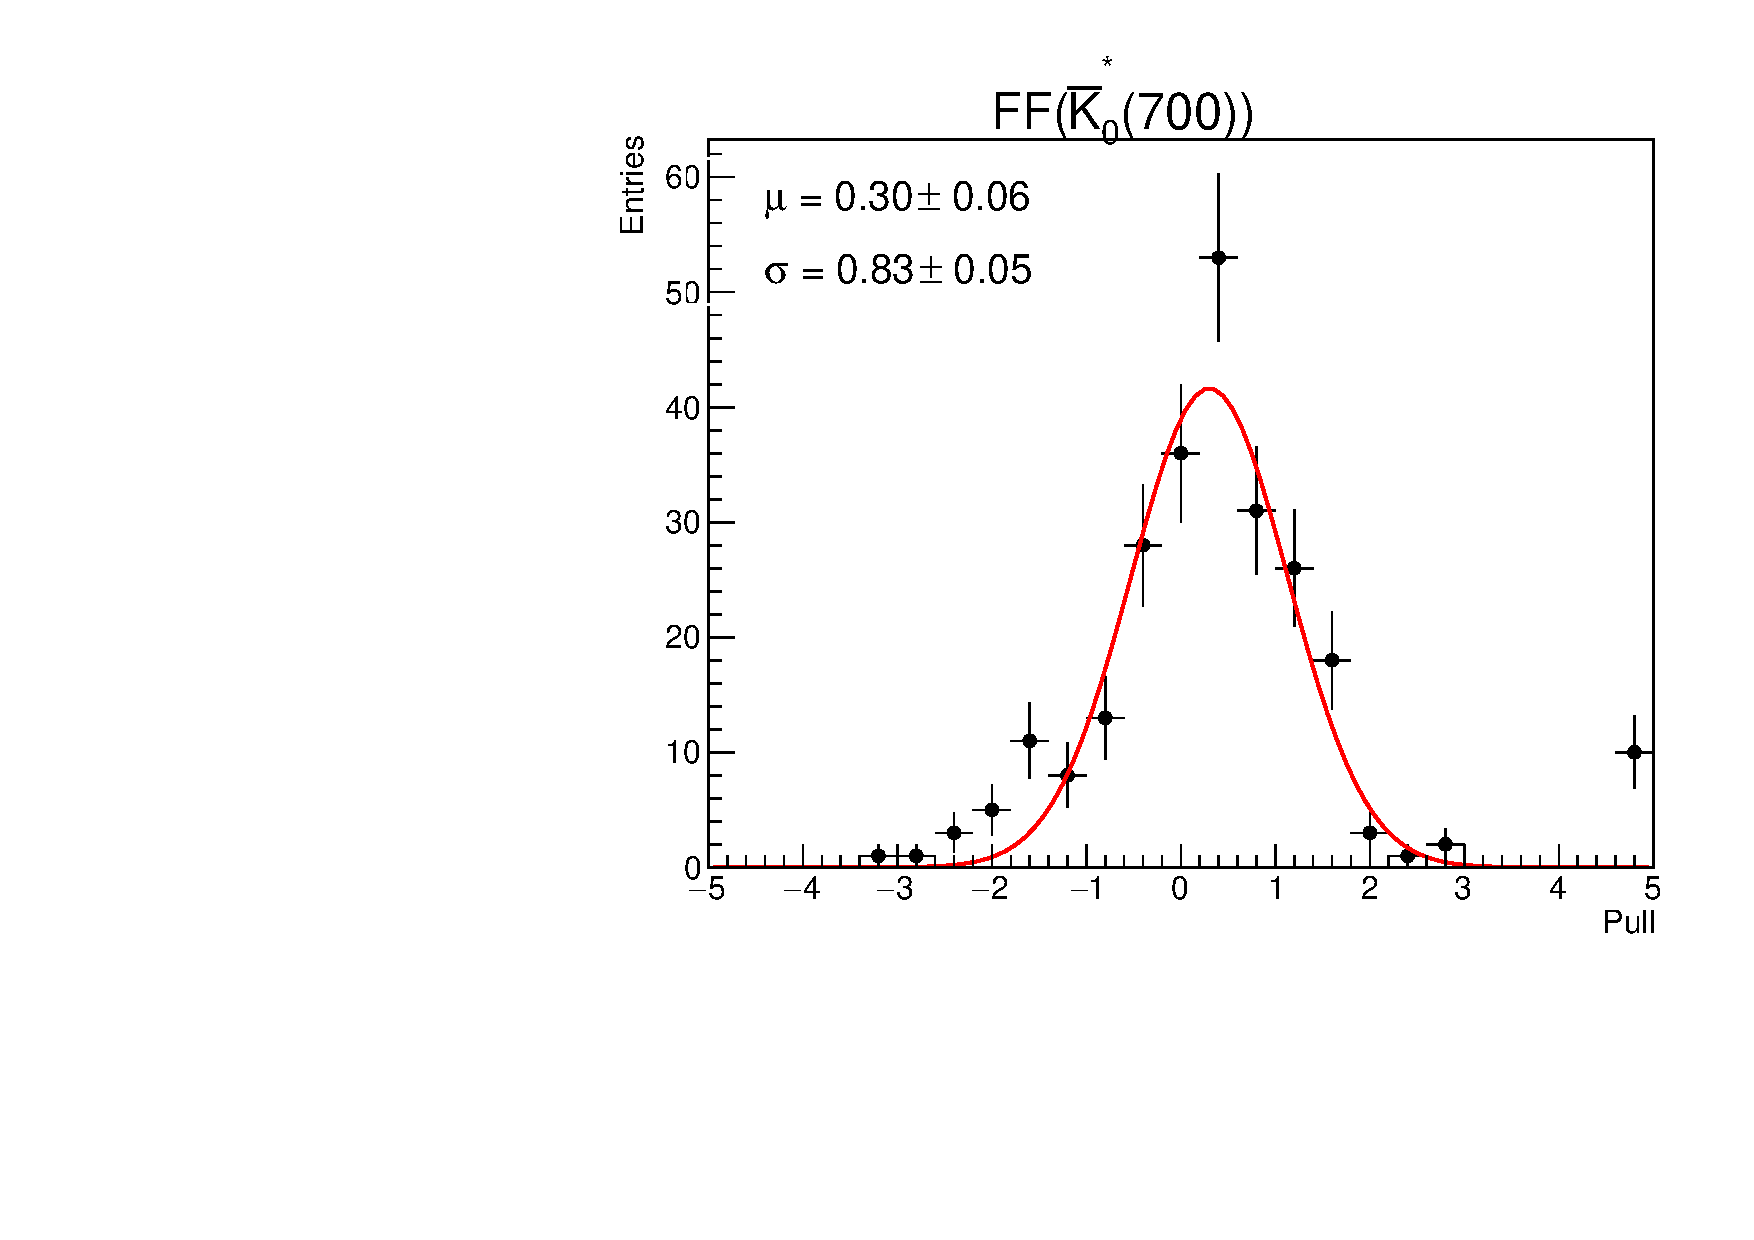
\includegraphics[width=0.24\textwidth]{figure/io_full_sim/fitfrac/pull_fitfrac_res5_comb.pdf}
    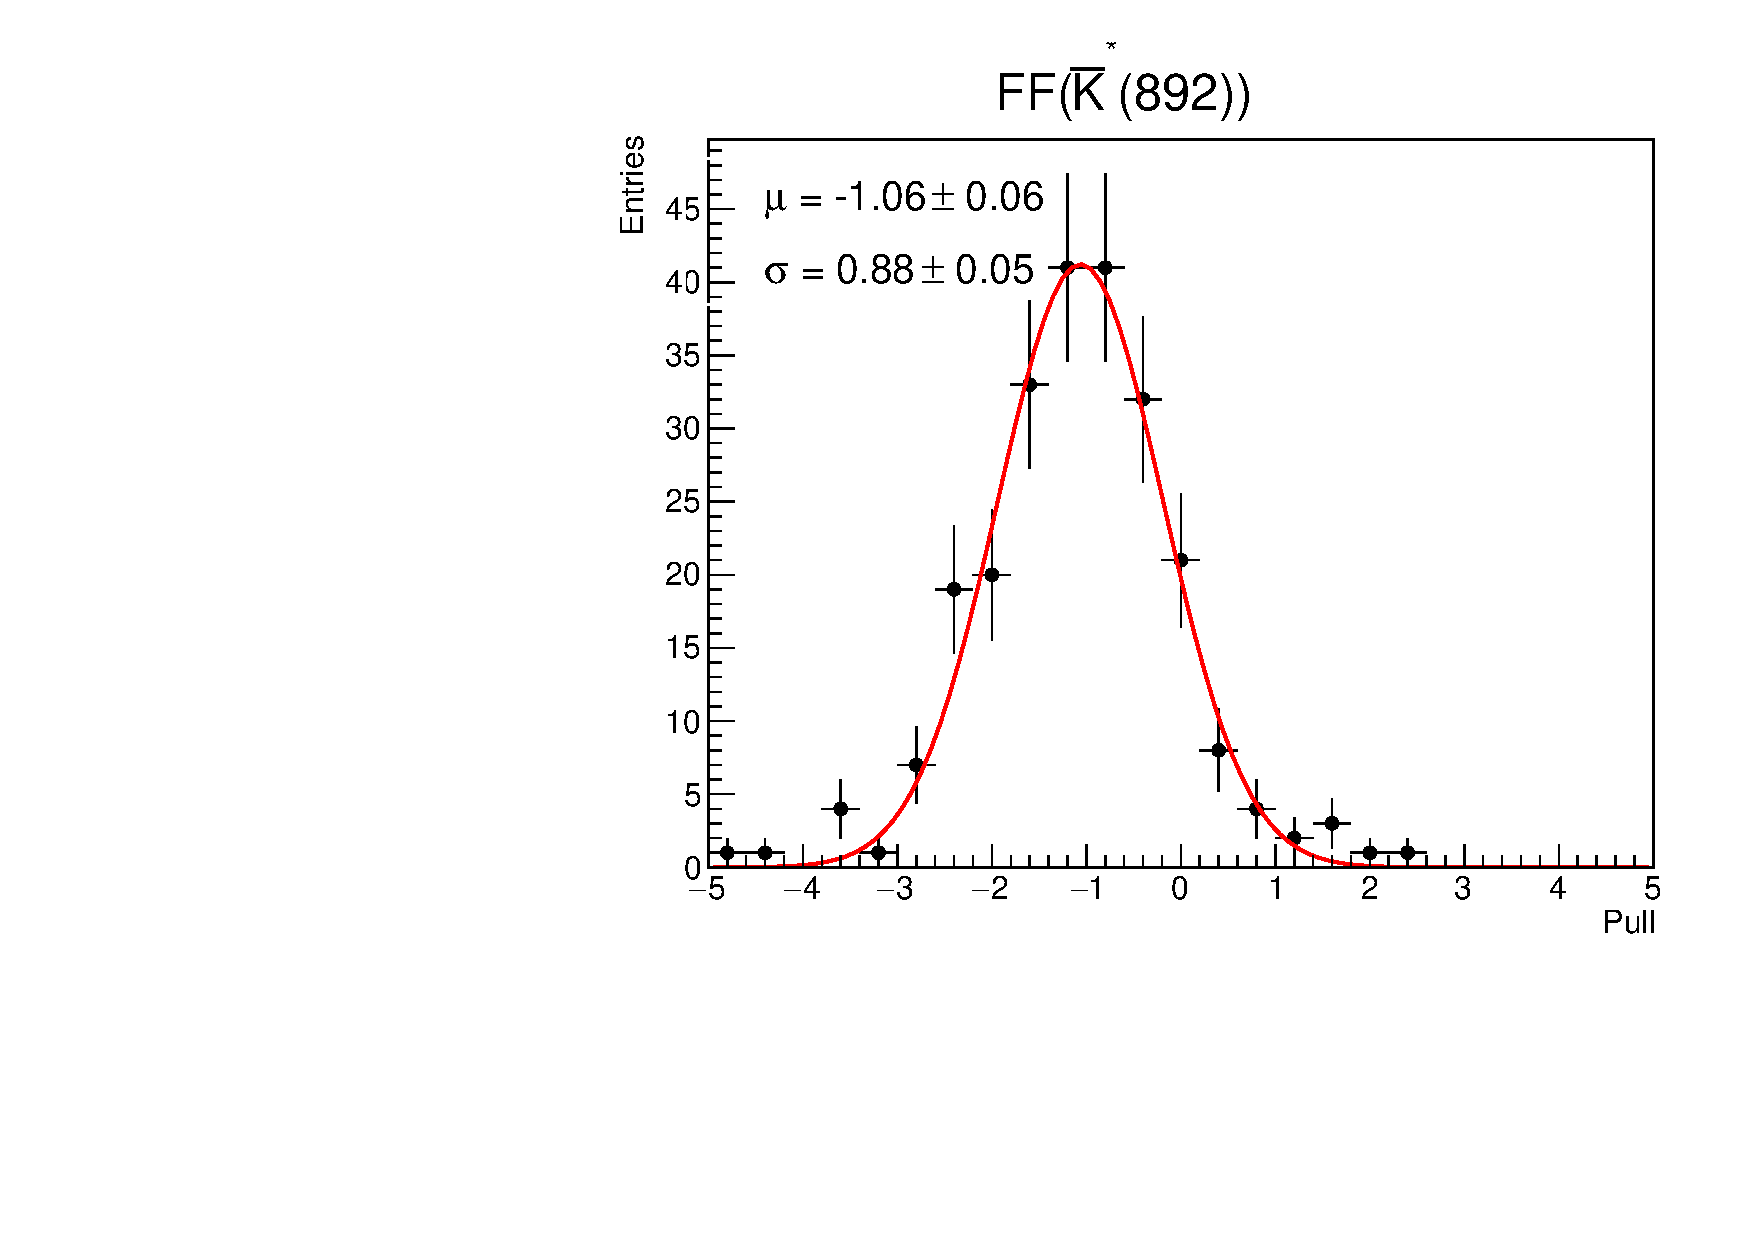
\includegraphics[width=0.24\textwidth]{figure/io_full_sim/fitfrac/pull_fitfrac_res6_comb.pdf}
    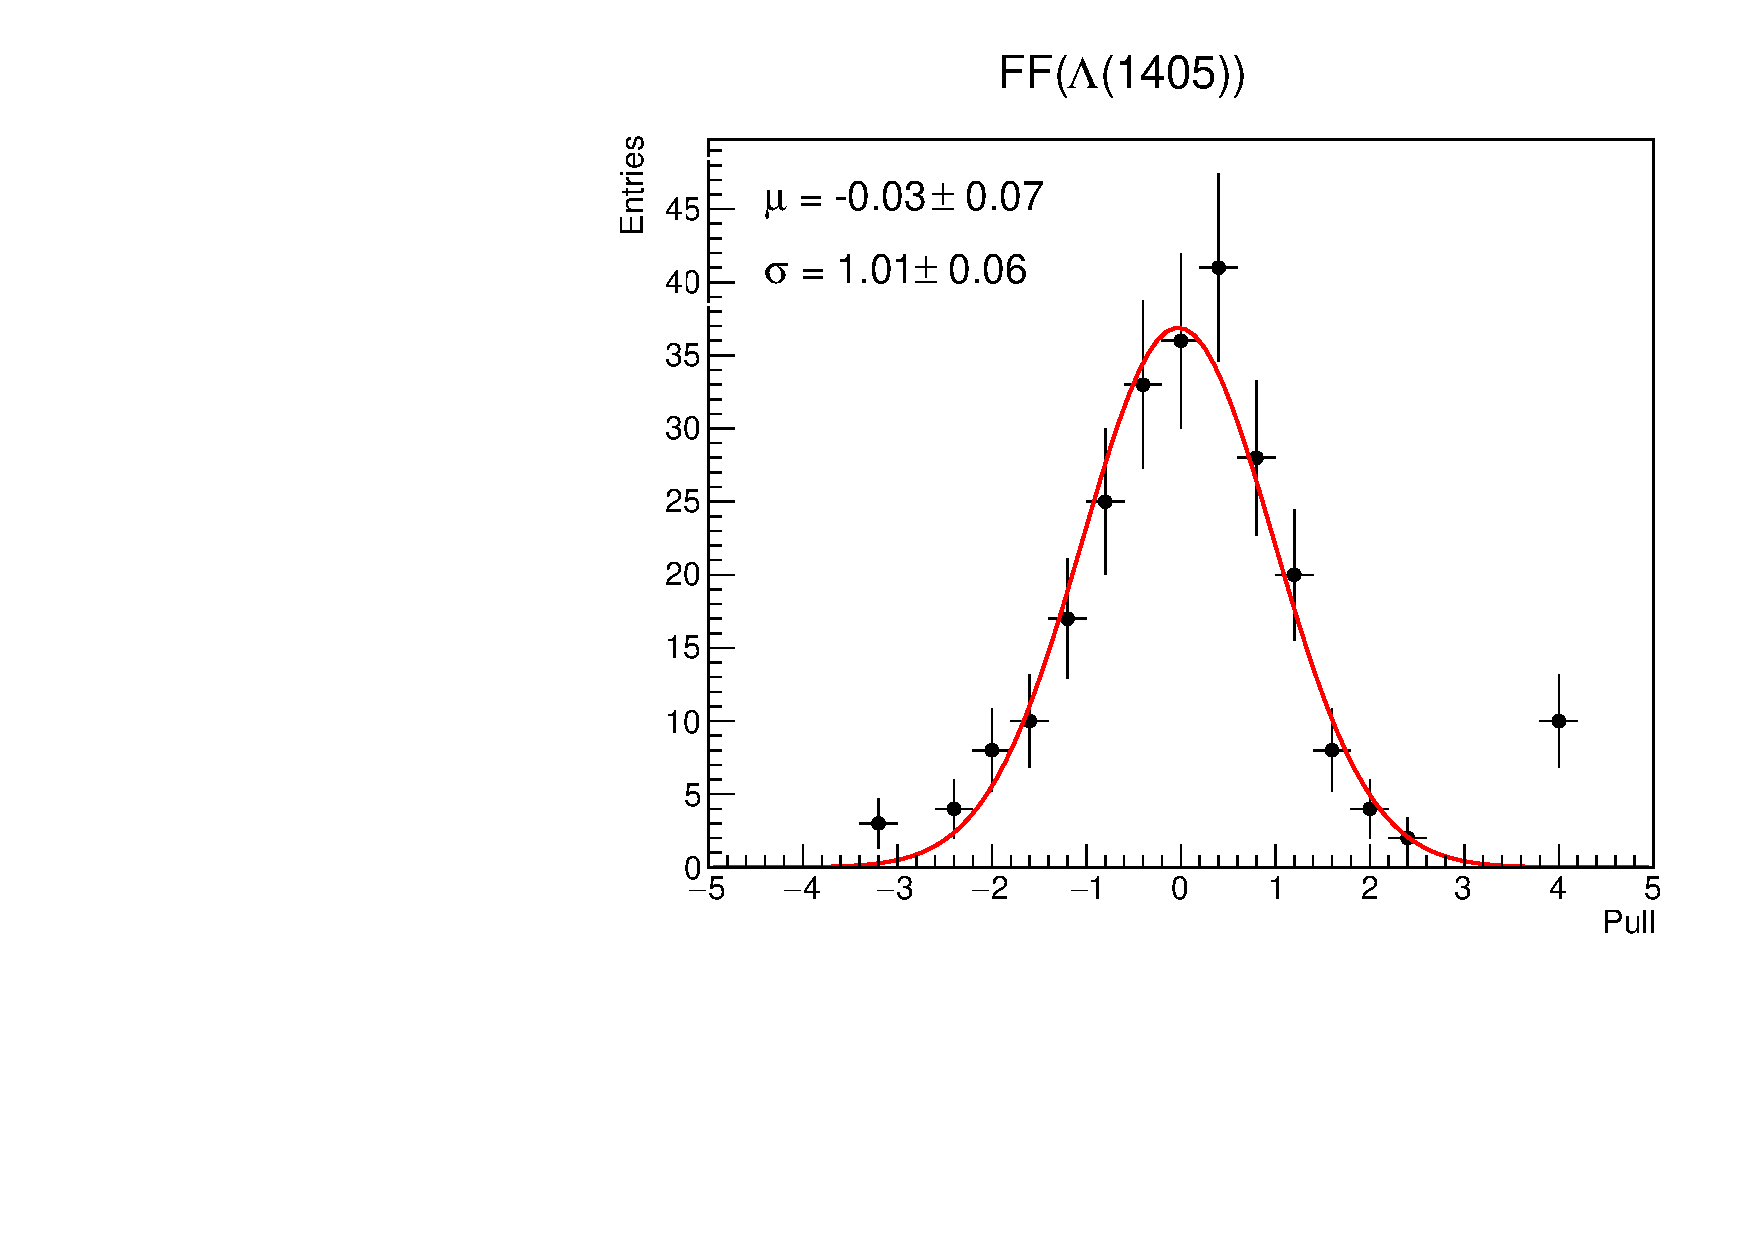
\includegraphics[width=0.24\textwidth]{figure/io_full_sim/fitfrac/pull_fitfrac_res7_comb.pdf}
    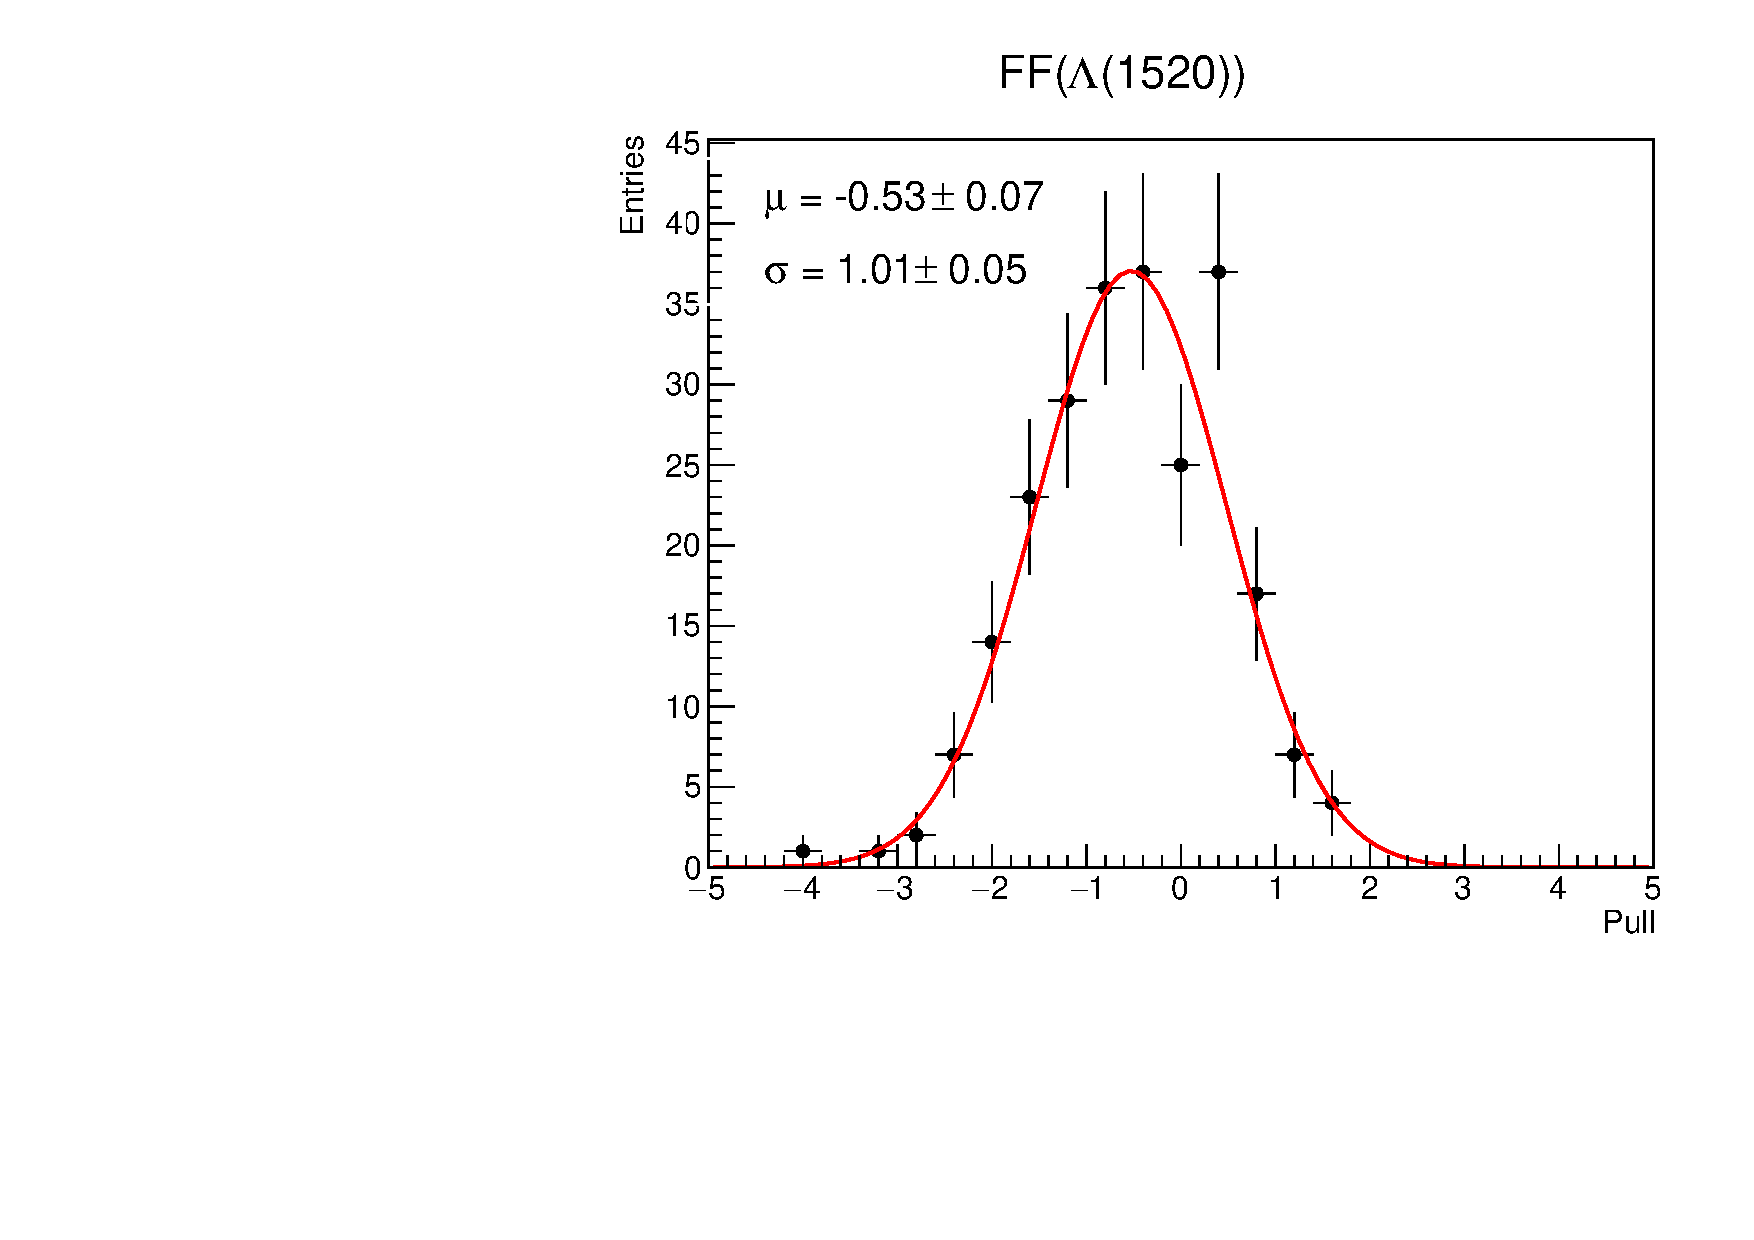
\includegraphics[width=0.24\textwidth]{figure/io_full_sim/fitfrac/pull_fitfrac_res8_comb.pdf}
    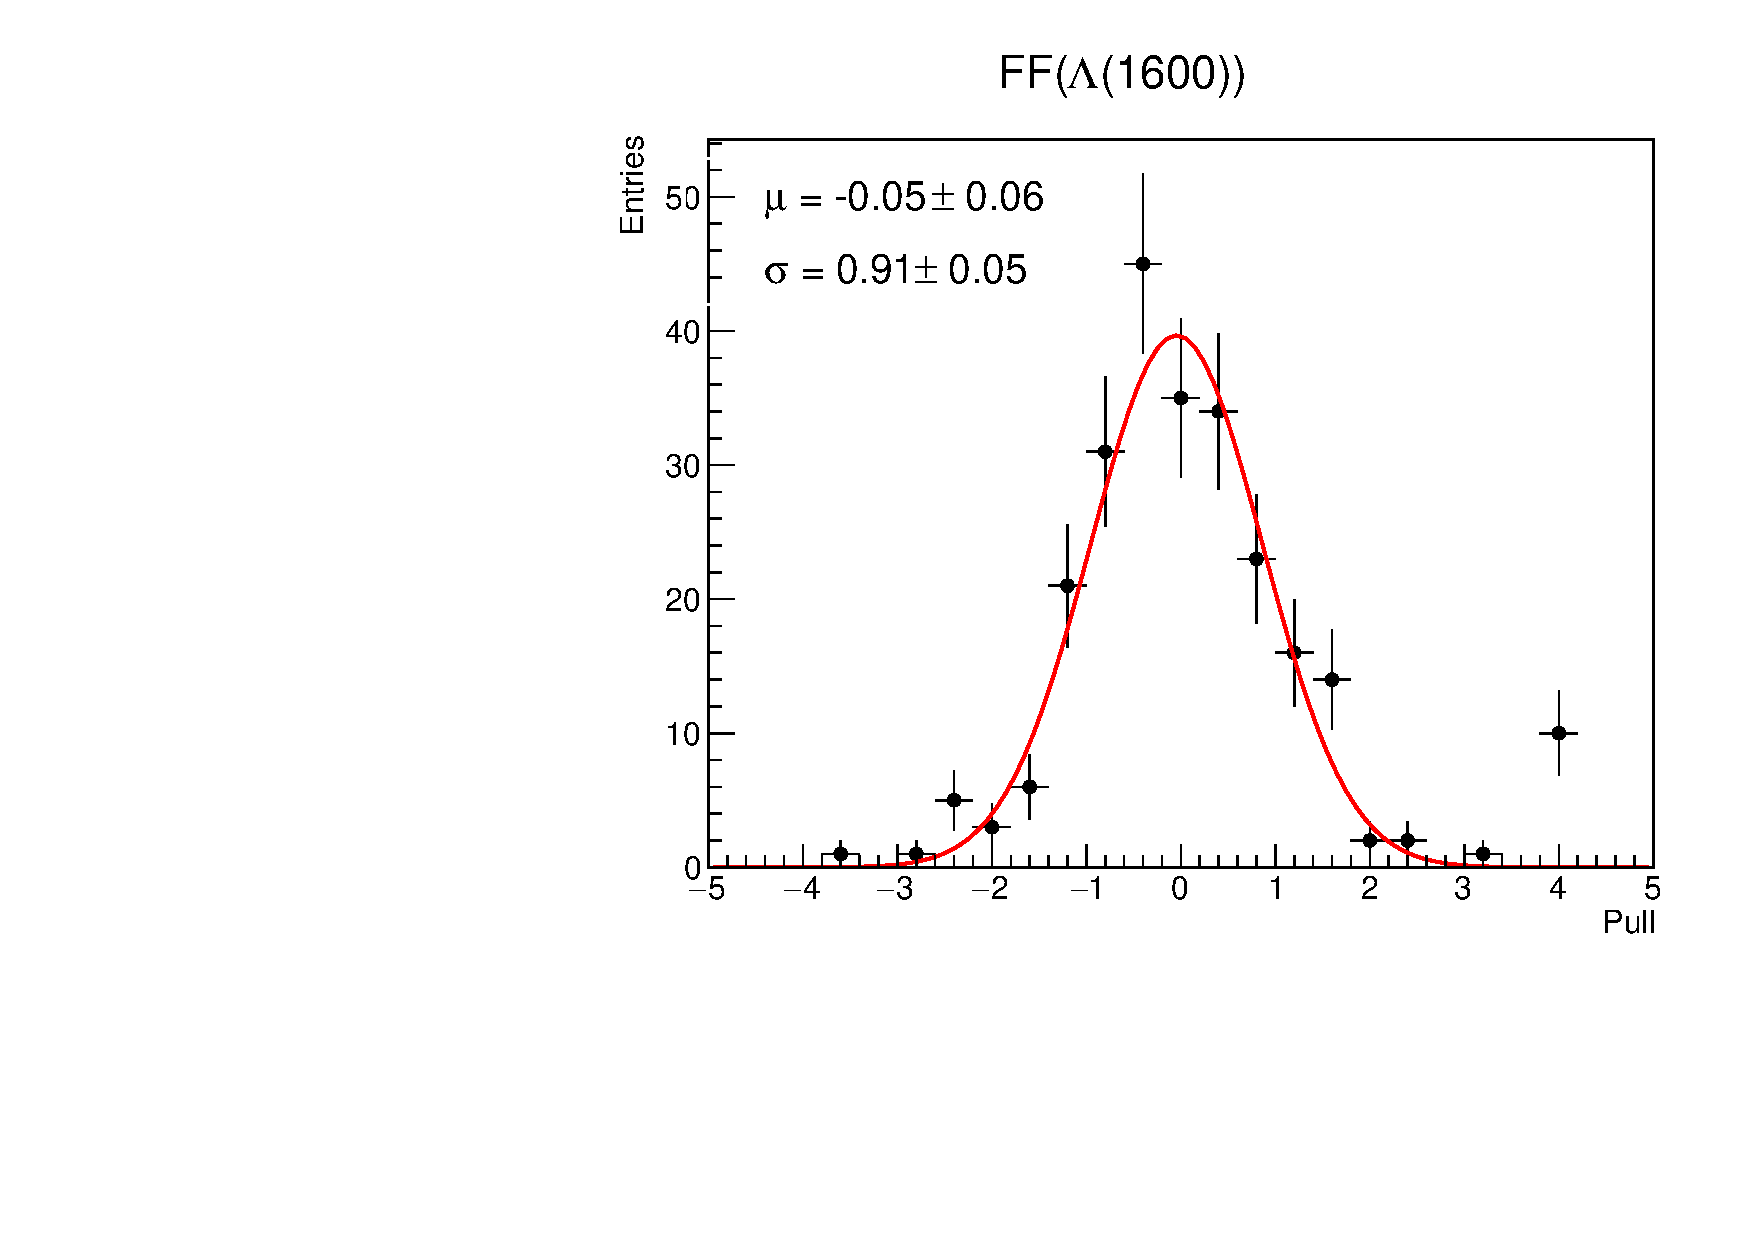
\includegraphics[width=0.24\textwidth]{figure/io_full_sim/fitfrac/pull_fitfrac_res9_comb.pdf}
    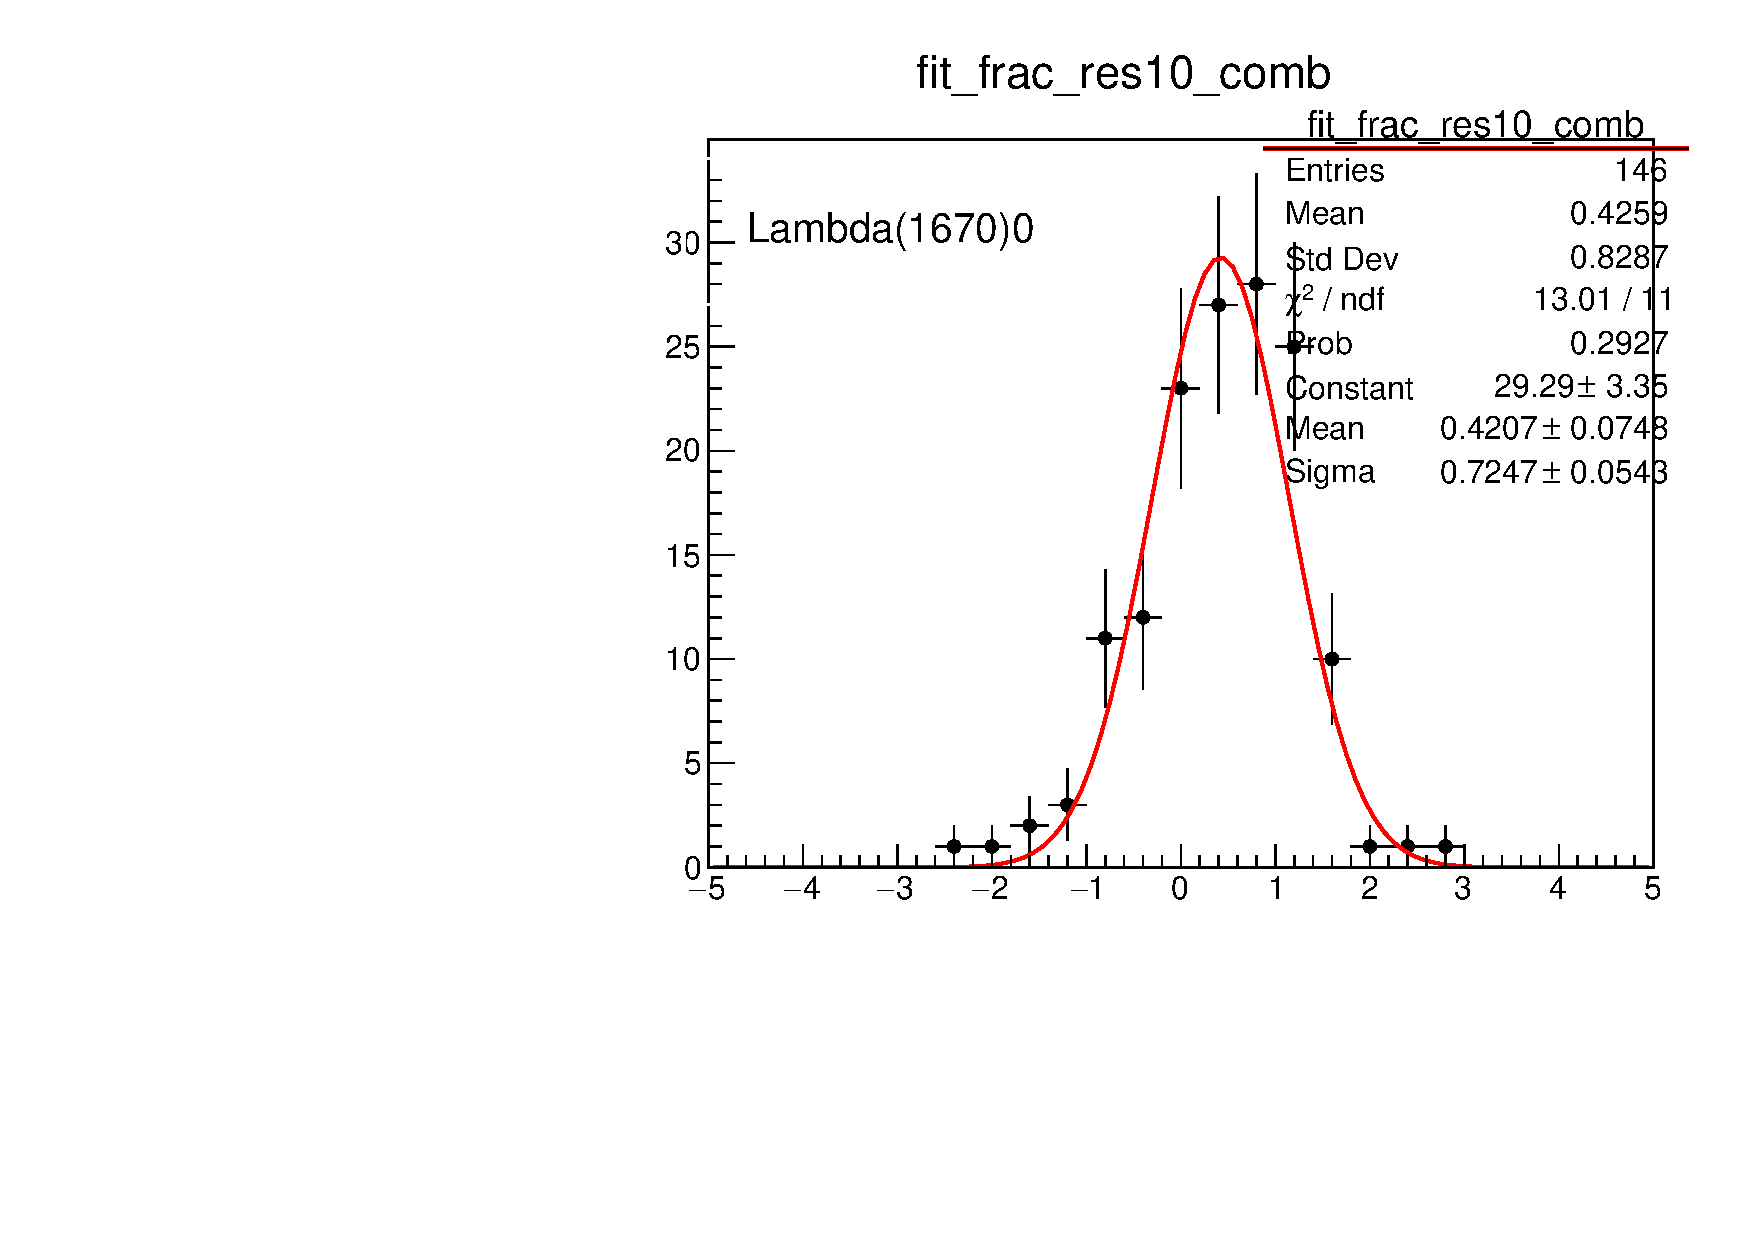
\includegraphics[width=0.24\textwidth]{figure/io_full_sim/fitfrac/pull_fitfrac_res10_comb.pdf}
    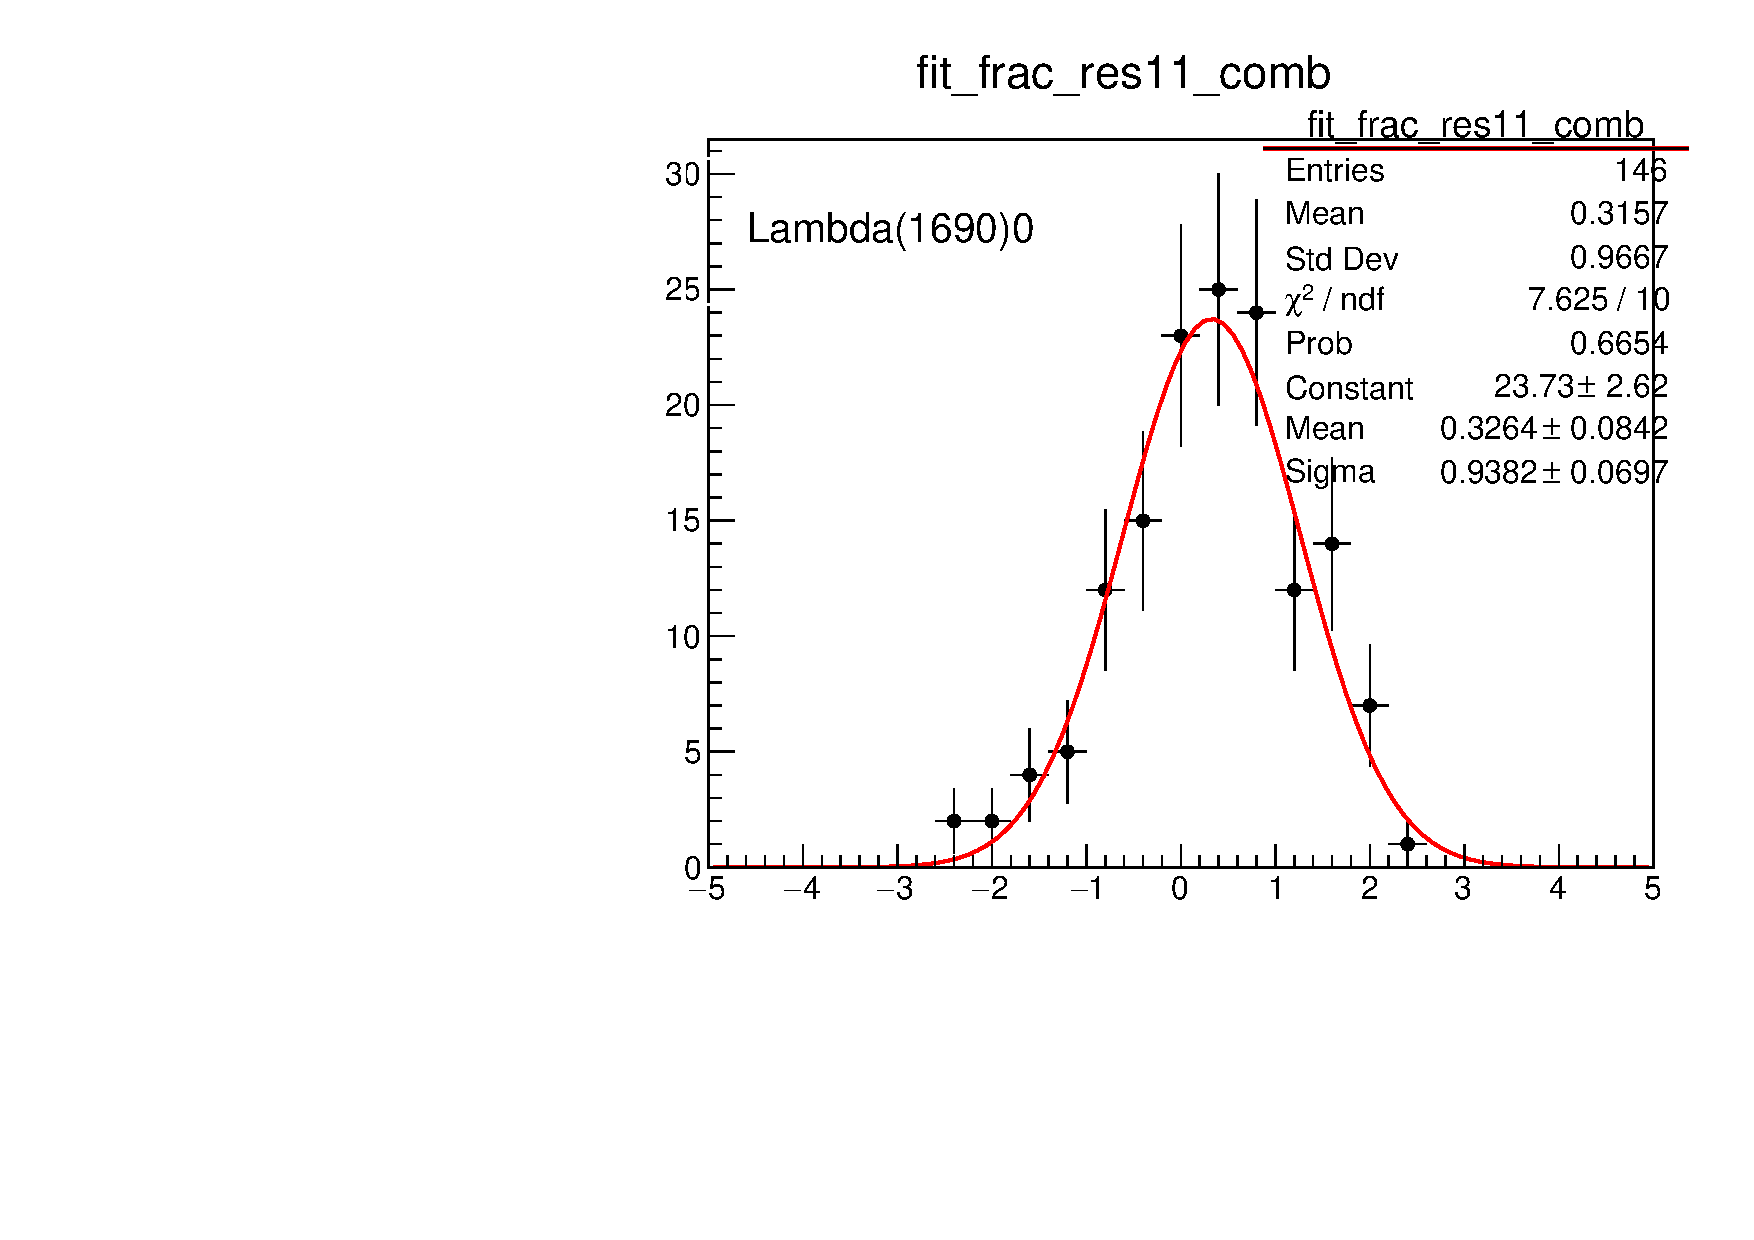
\includegraphics[width=0.24\textwidth]{figure/io_full_sim/fitfrac/pull_fitfrac_res11_comb.pdf}
    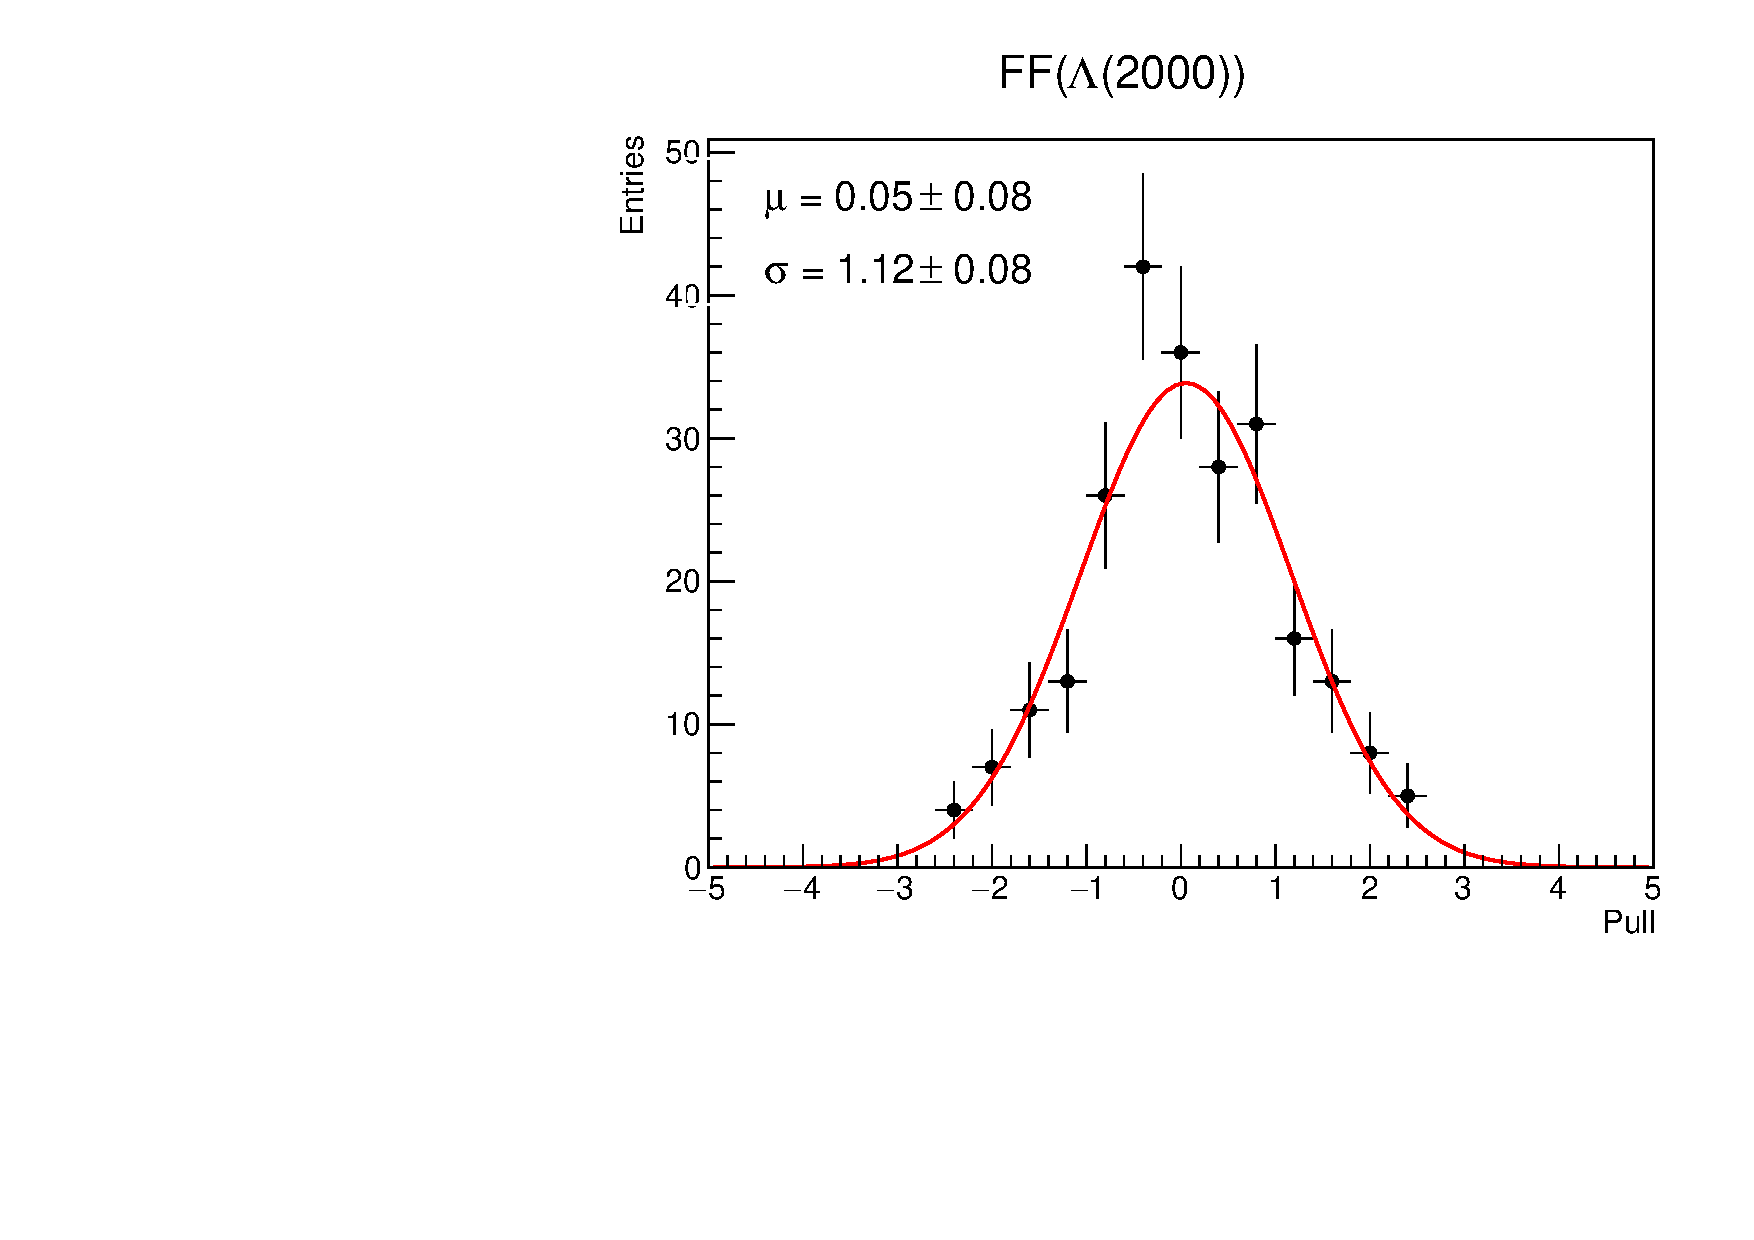
\includegraphics[width=0.24\textwidth]{figure/io_full_sim/fitfrac/pull_fitfrac_res12_comb.pdf}
    \caption{Pull distributions of FF for each resonance.}
\label{fig:io_wo_bkg_pull_ff}
\end{figure}

\begin{figure}[h]\centering
    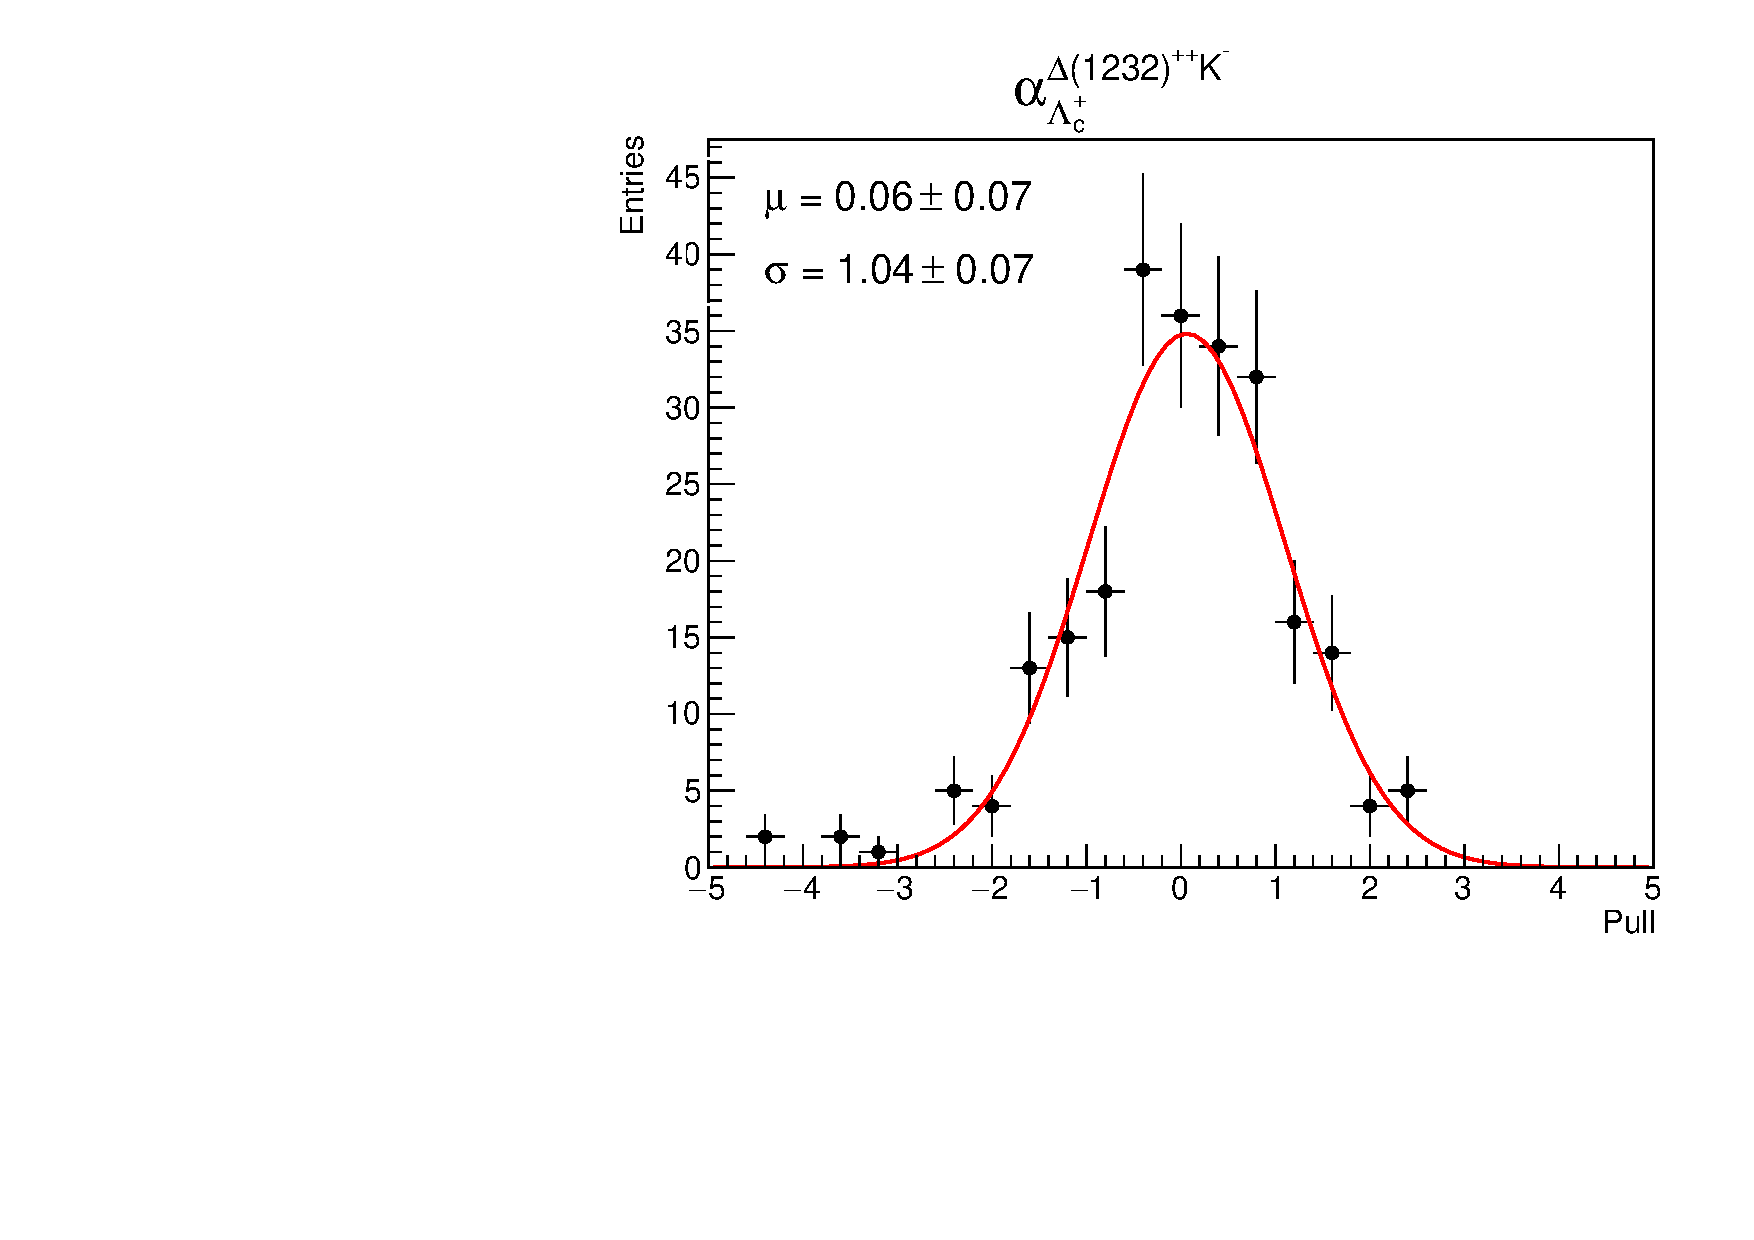
\includegraphics[width=0.24\textwidth]{figure/io_full_sim/alpha/pull_alpha_Delta_1232_pp.pdf}
    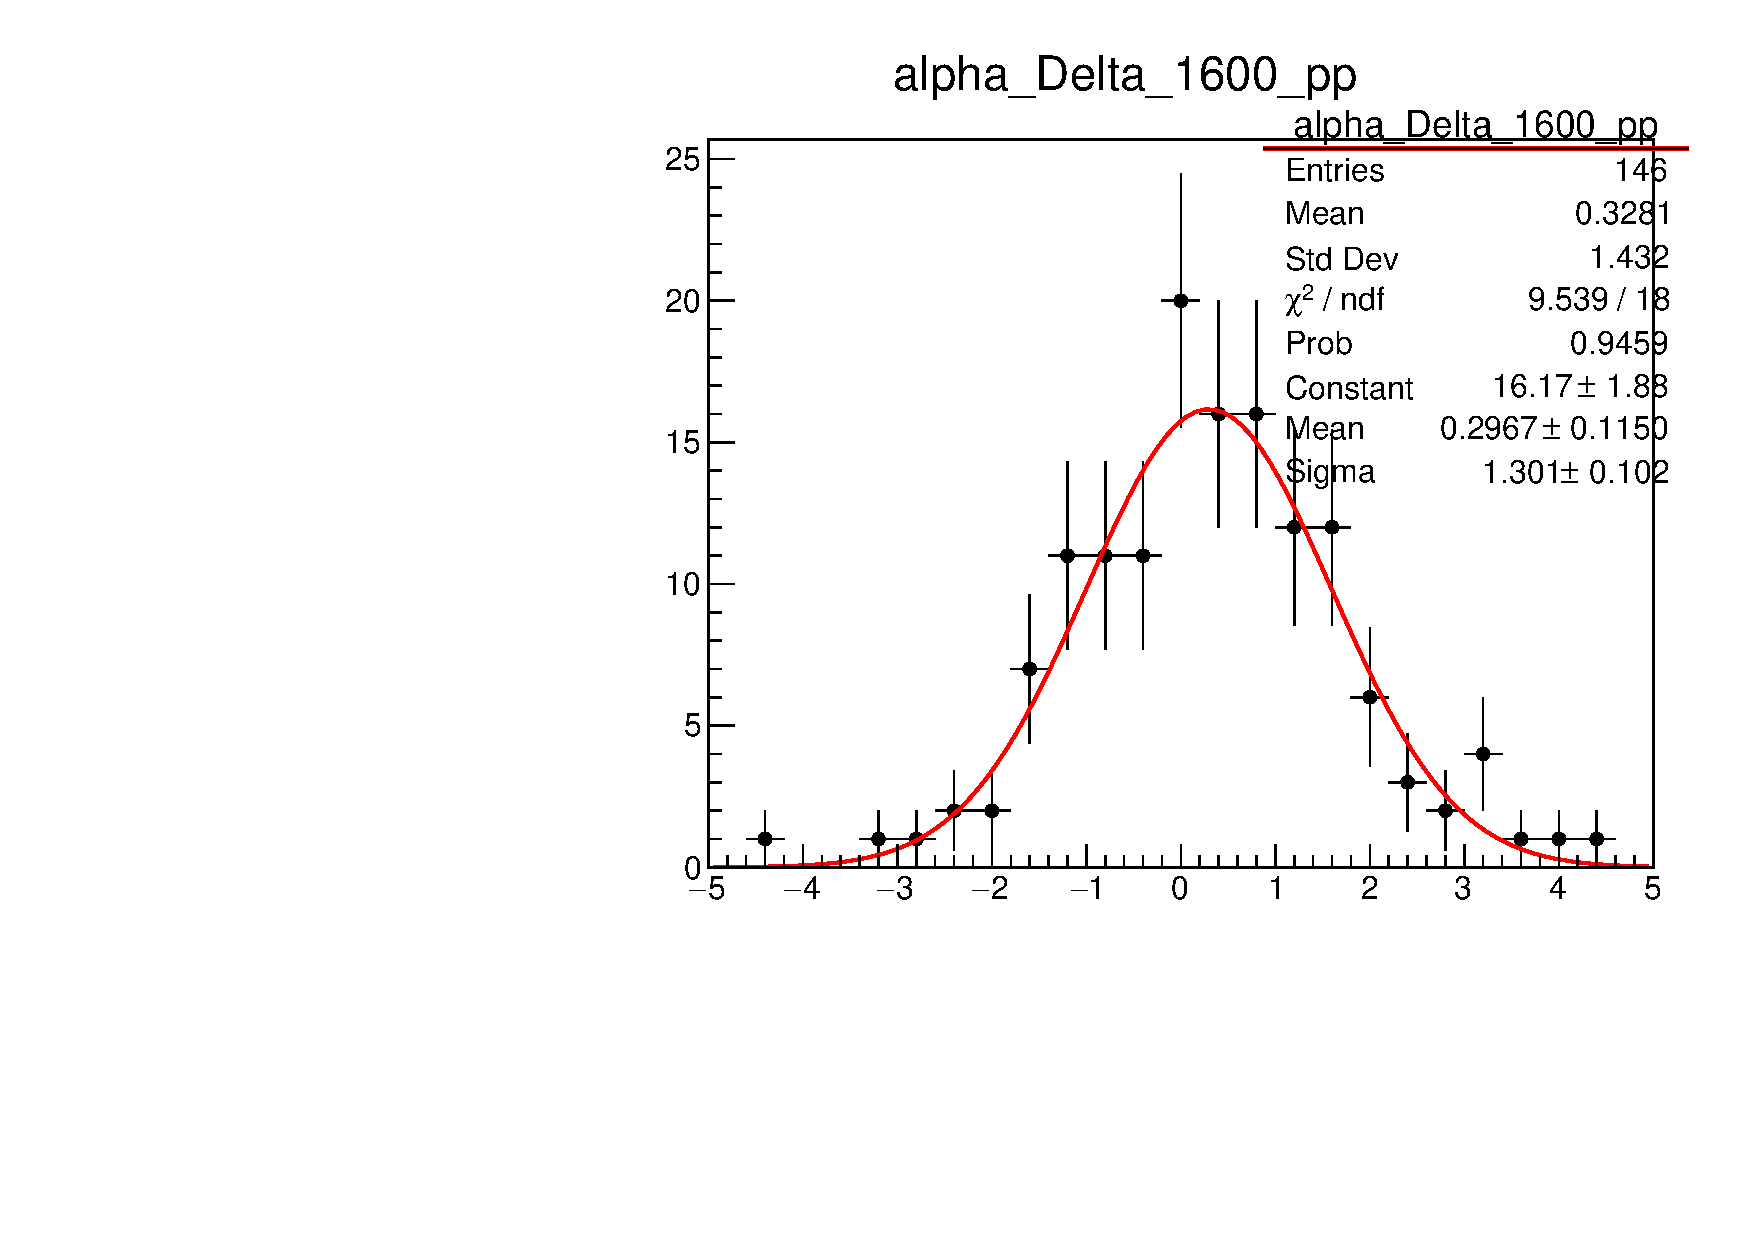
\includegraphics[width=0.24\textwidth]{figure/io_full_sim/alpha/pull_alpha_Delta_1600_pp.pdf}
    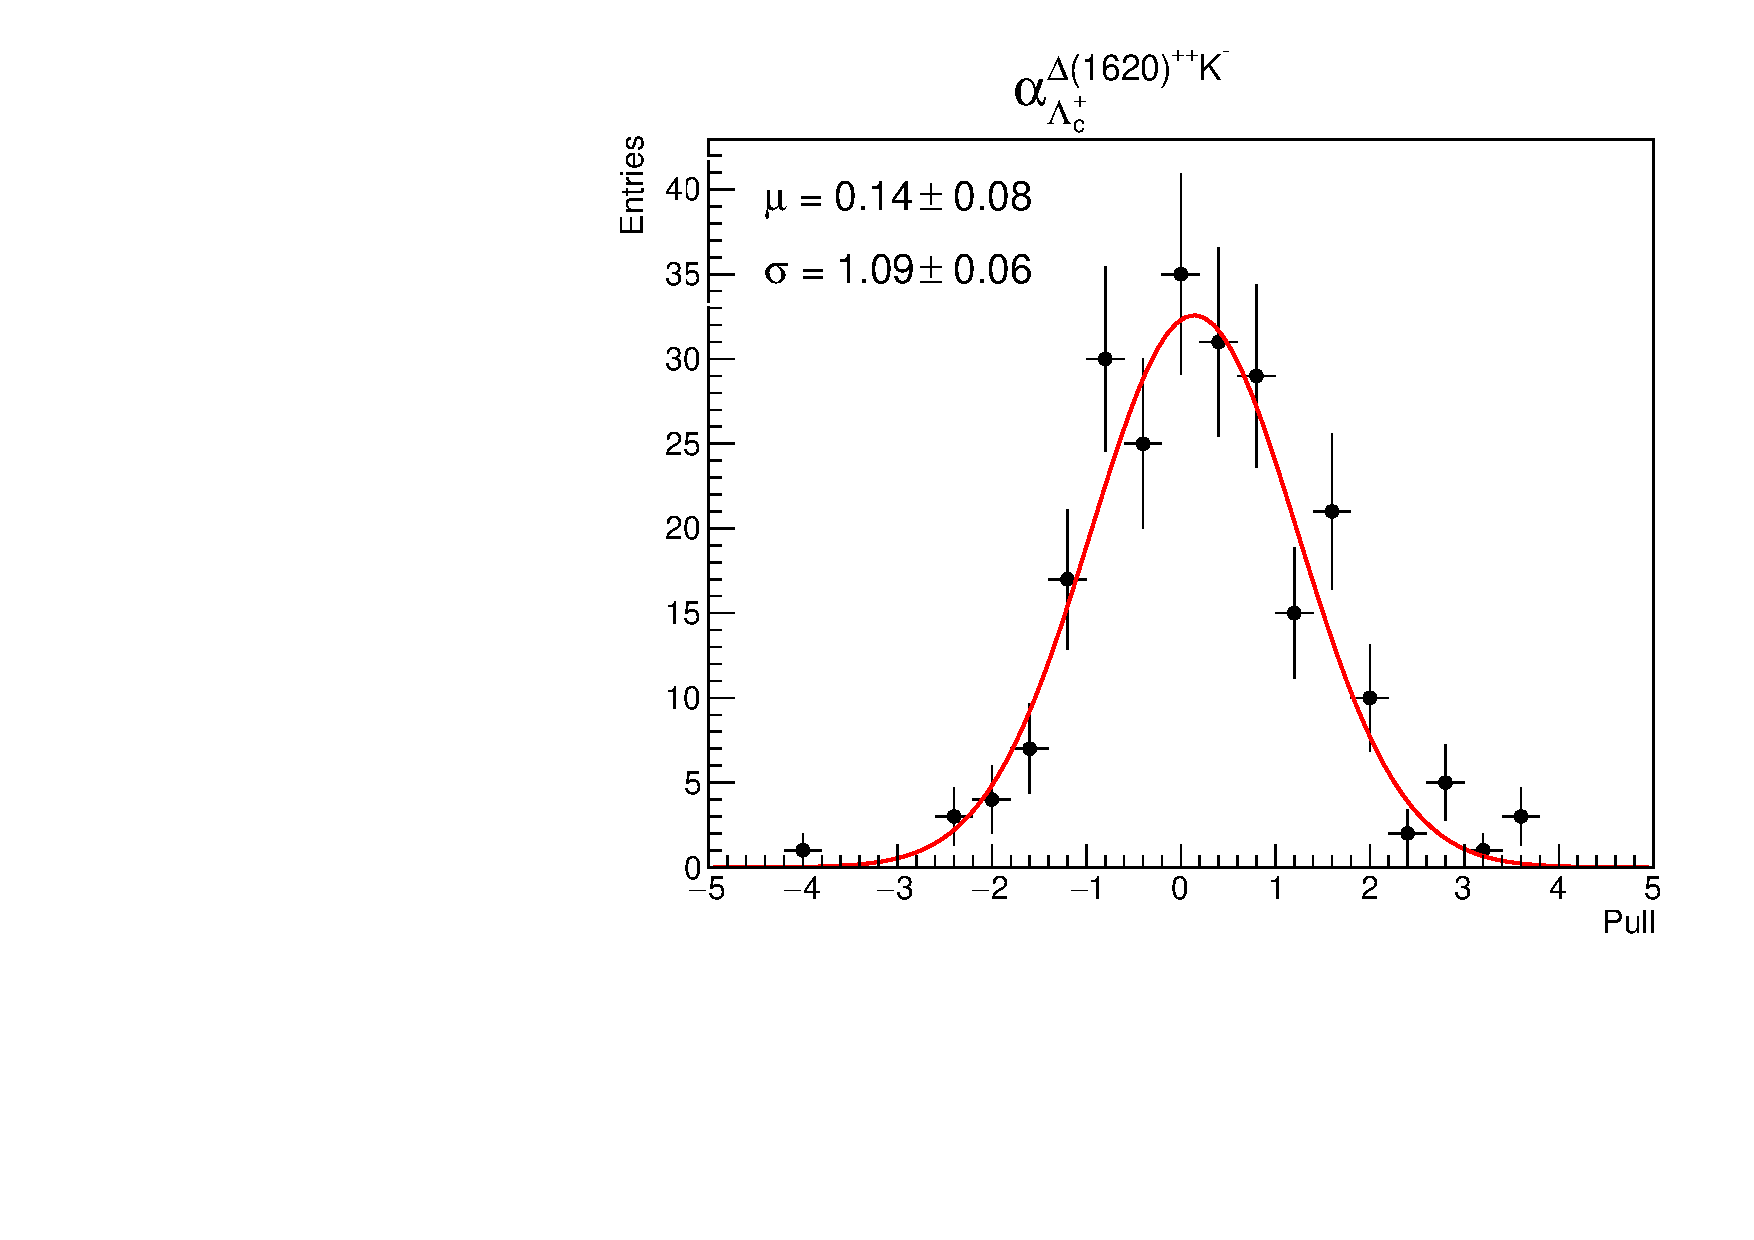
\includegraphics[width=0.24\textwidth]{figure/io_full_sim/alpha/pull_alpha_Delta_1620_pp.pdf}
    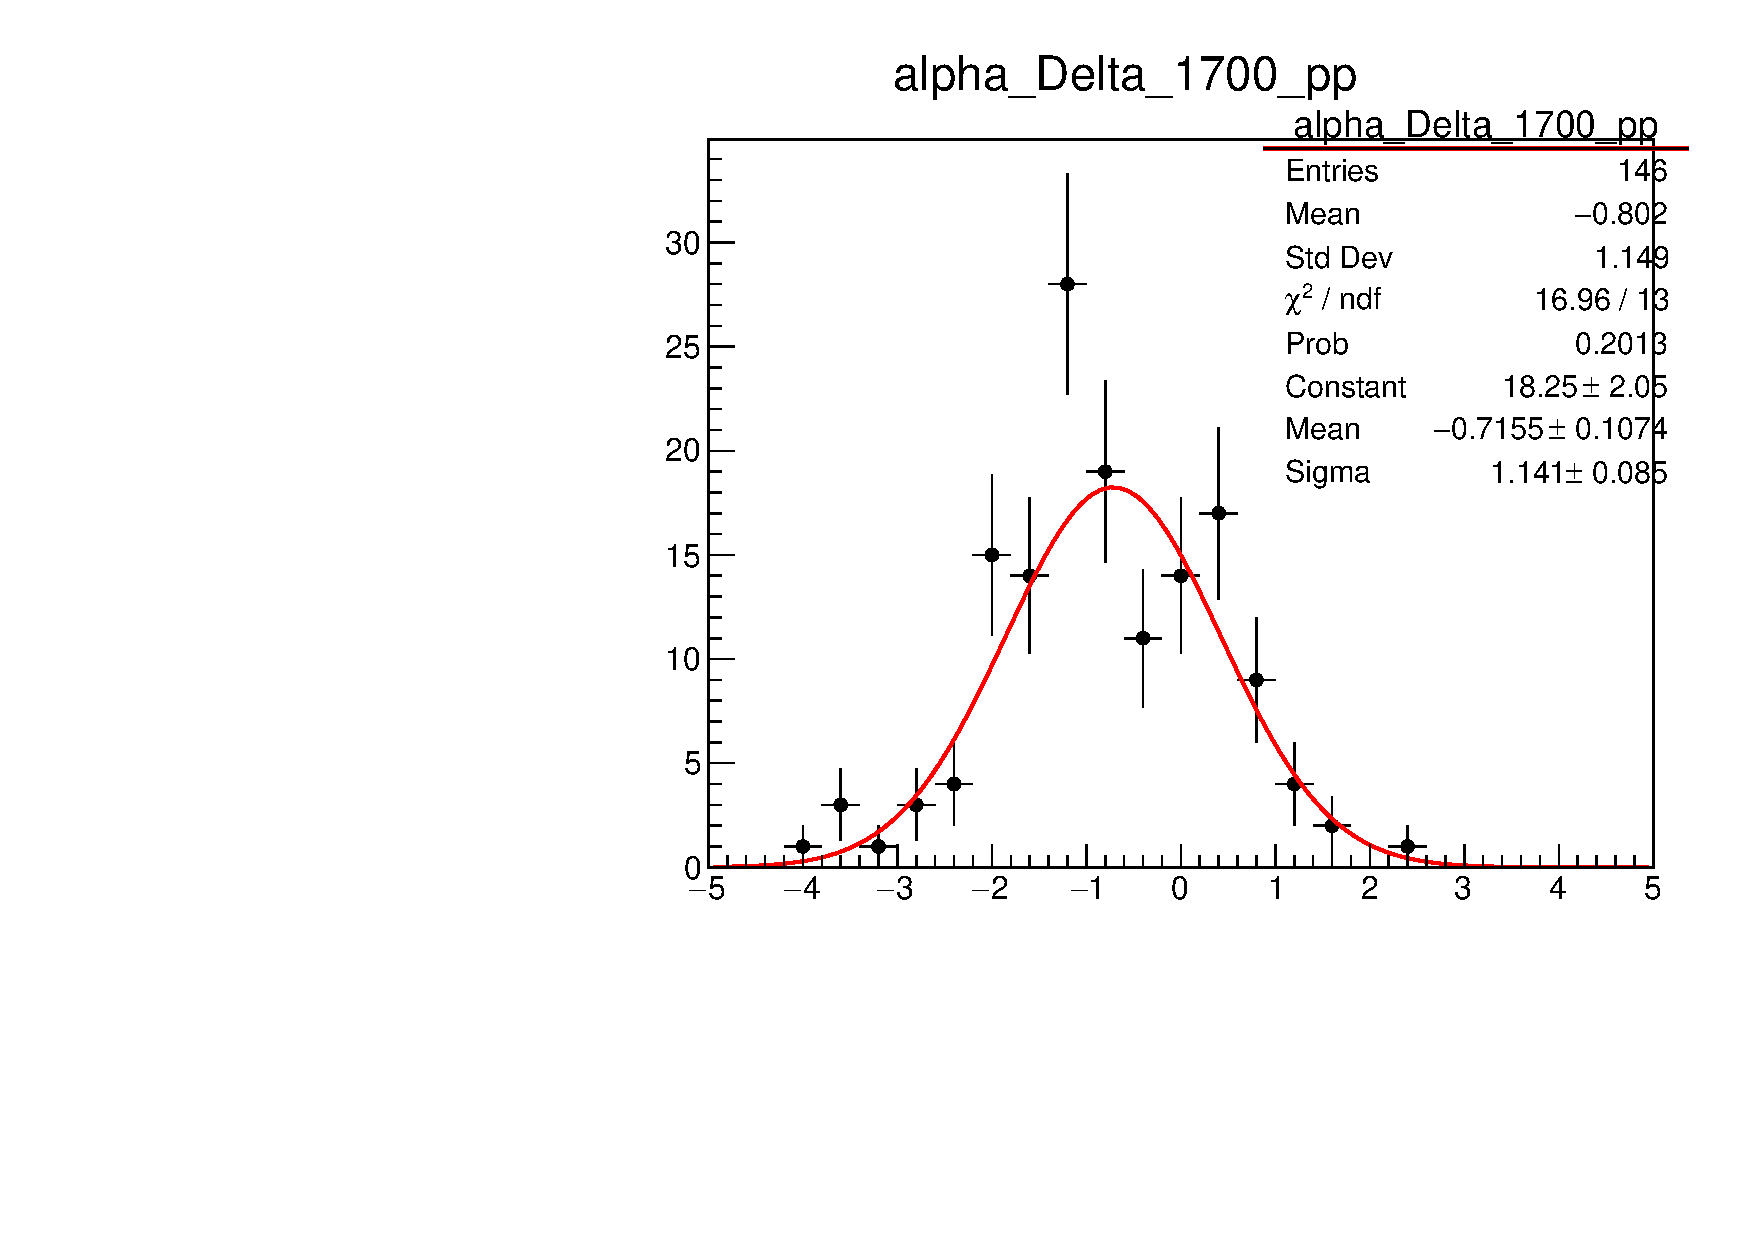
\includegraphics[width=0.24\textwidth]{figure/io_full_sim/alpha/pull_alpha_Delta_1700_pp.pdf}
    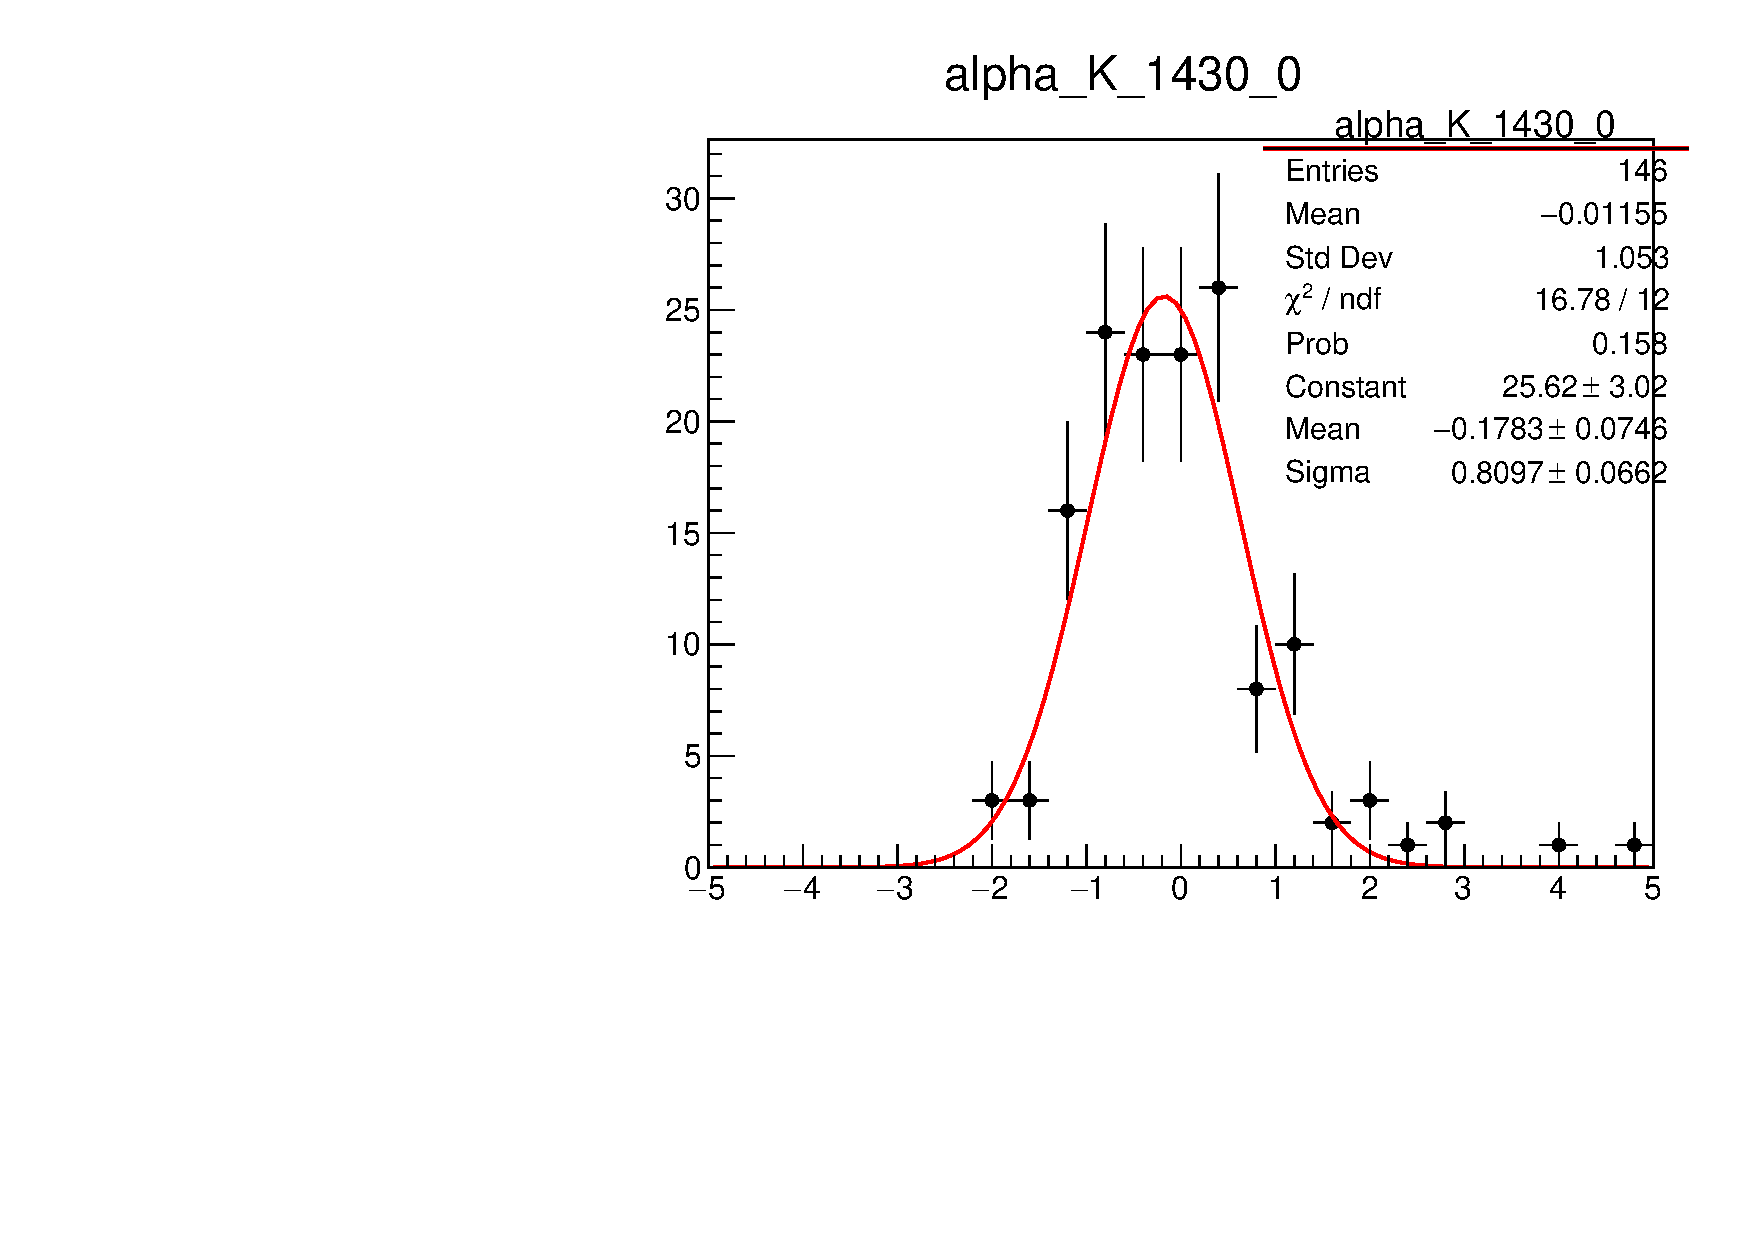
\includegraphics[width=0.24\textwidth]{figure/io_full_sim/alpha/pull_alpha_K_1430_0.pdf}
    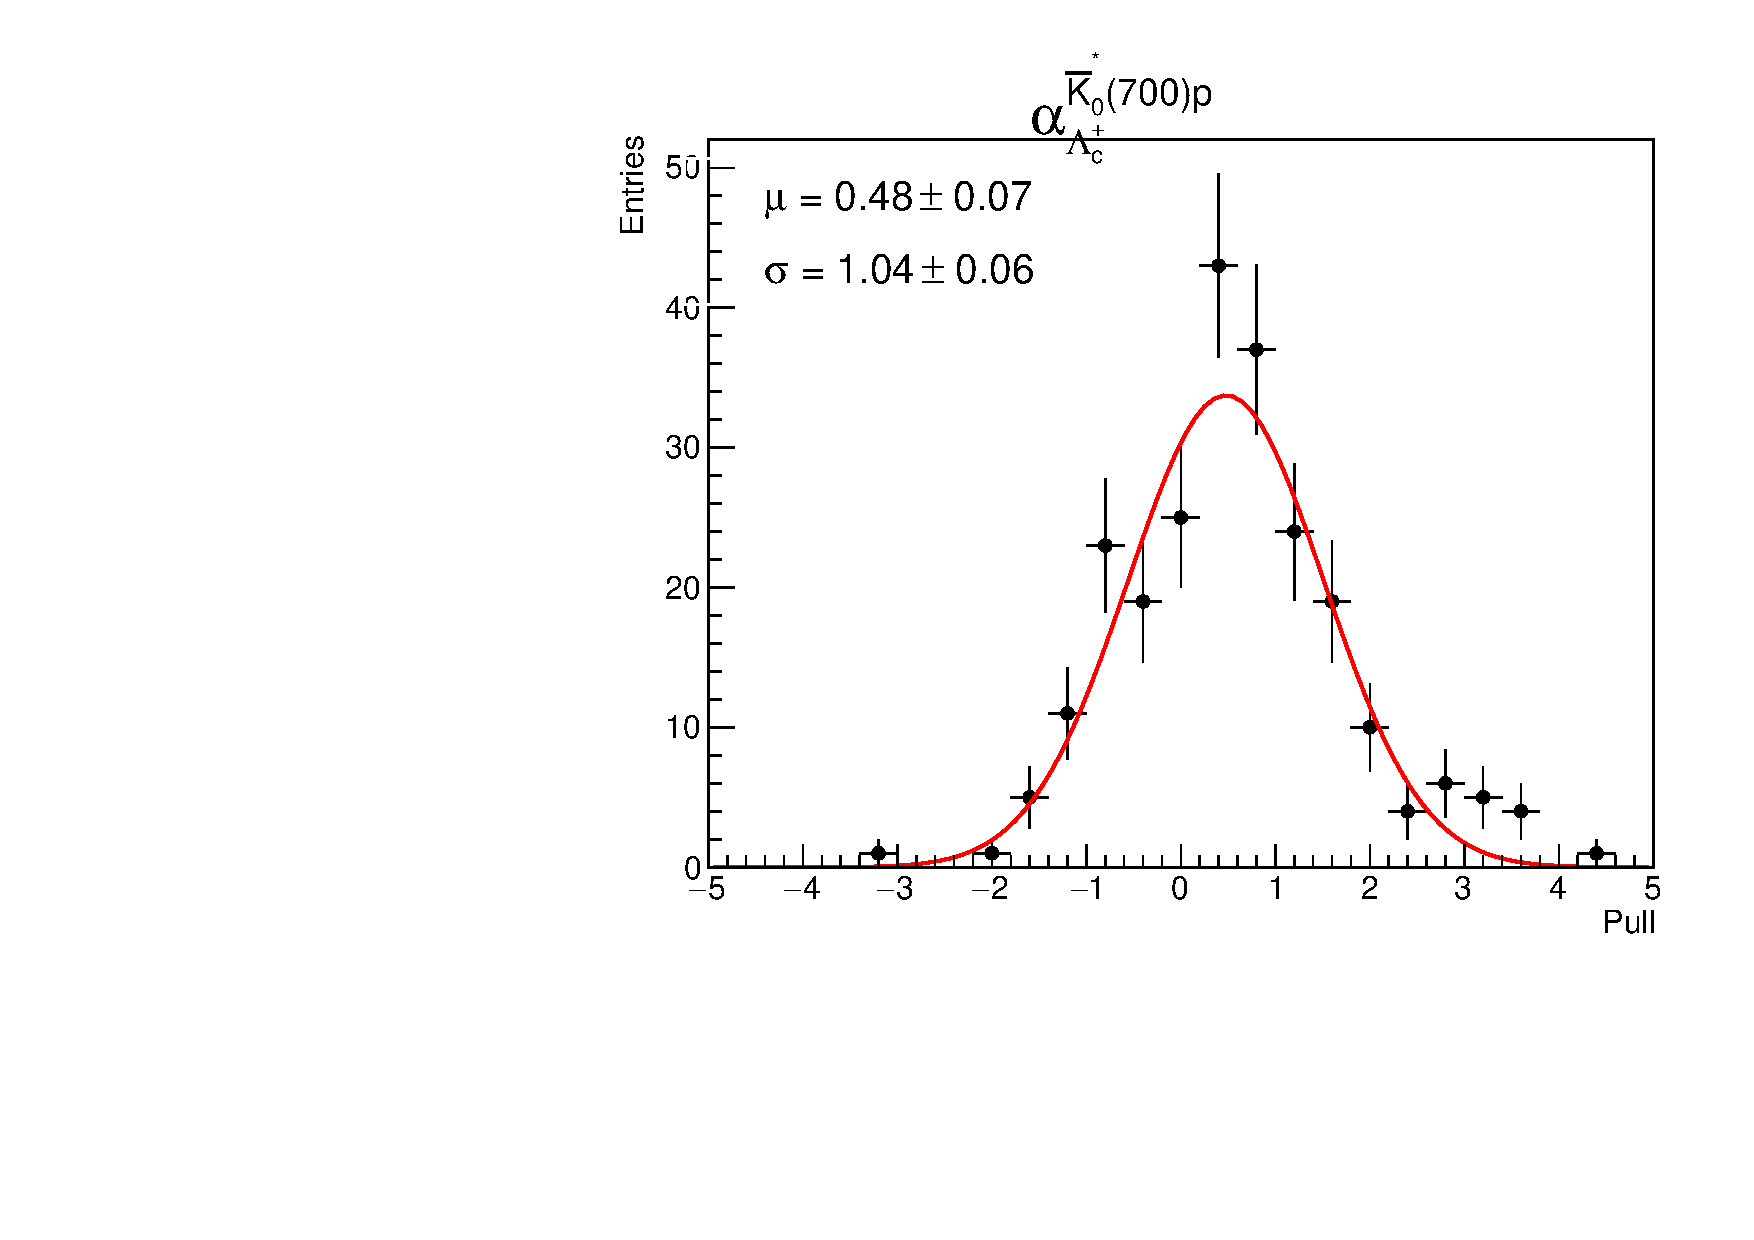
\includegraphics[width=0.24\textwidth]{figure/io_full_sim/alpha/pull_alpha_K_700_0.pdf}
    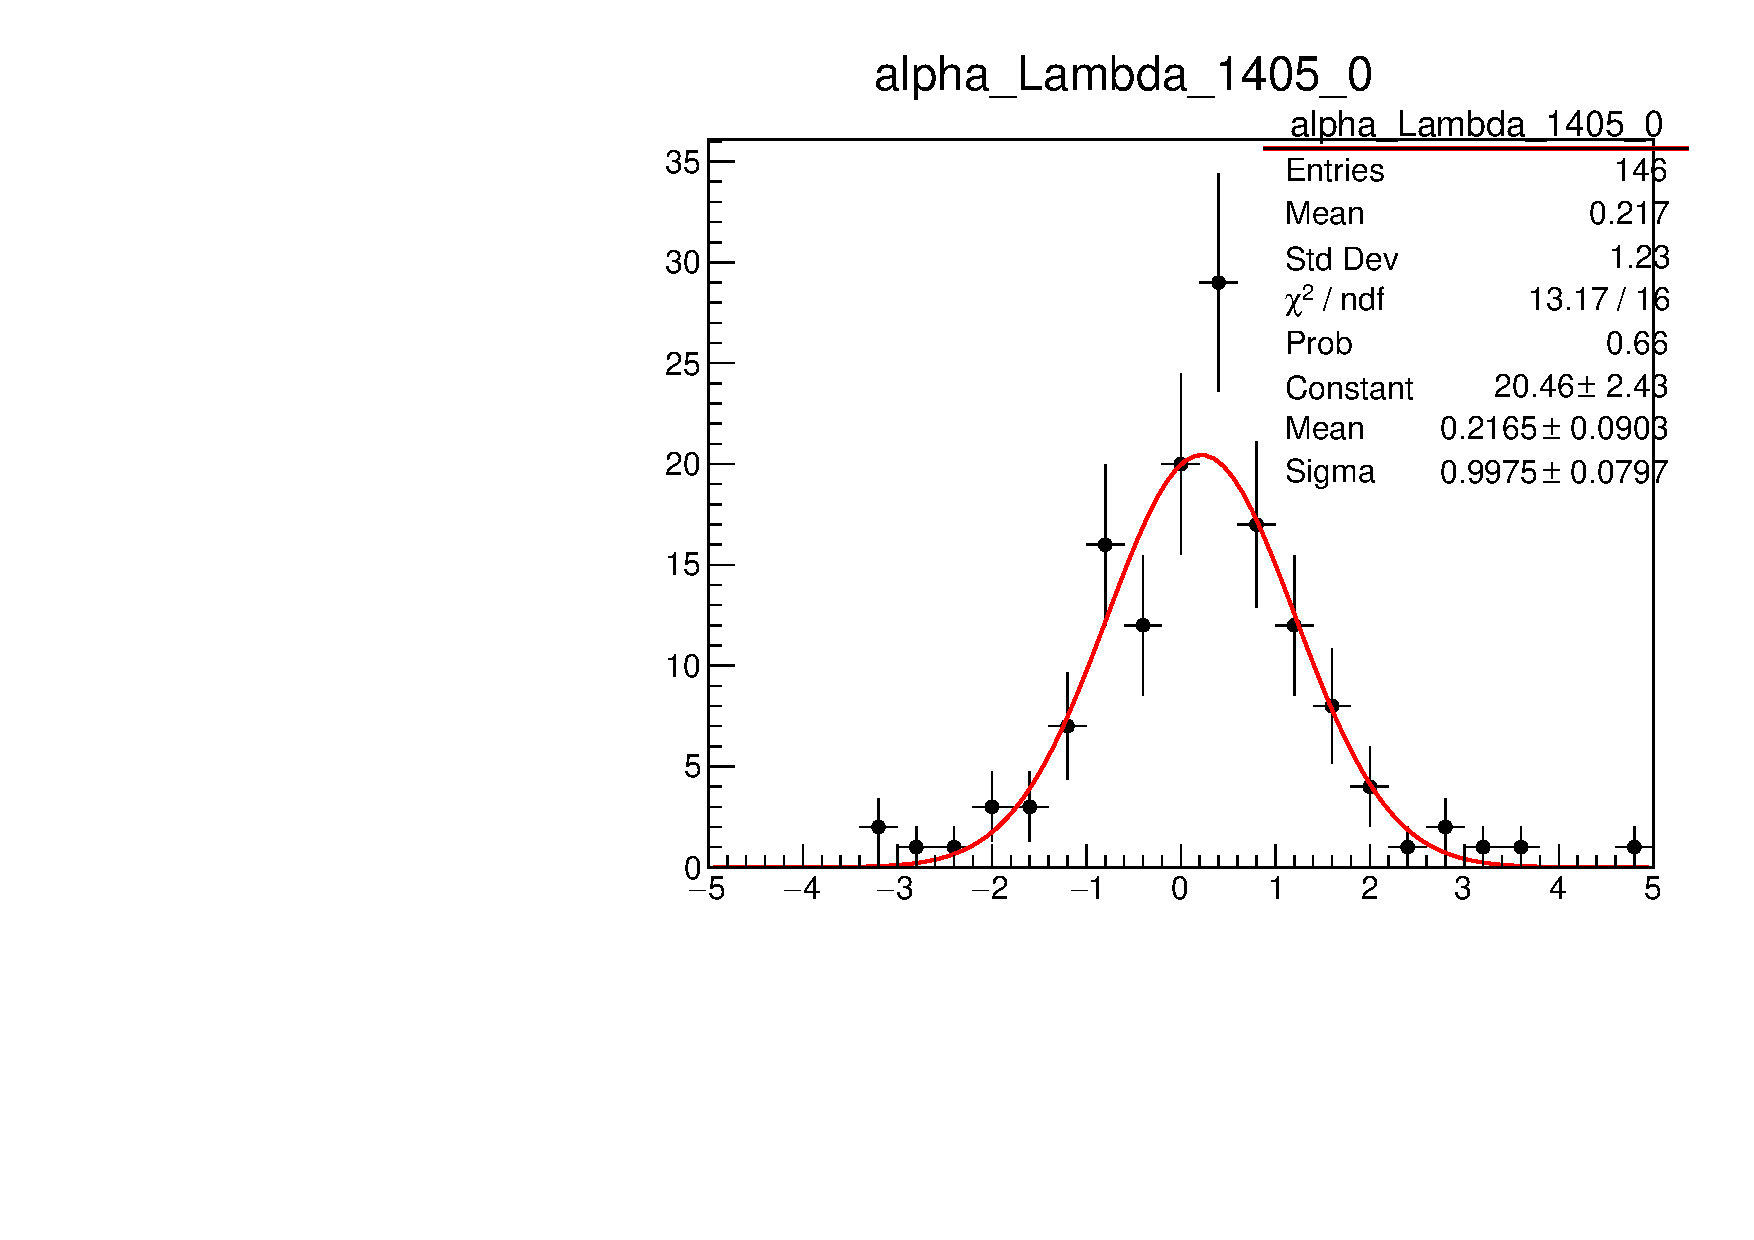
\includegraphics[width=0.24\textwidth]{figure/io_full_sim/alpha/pull_alpha_Lambda_1405_0.pdf}
    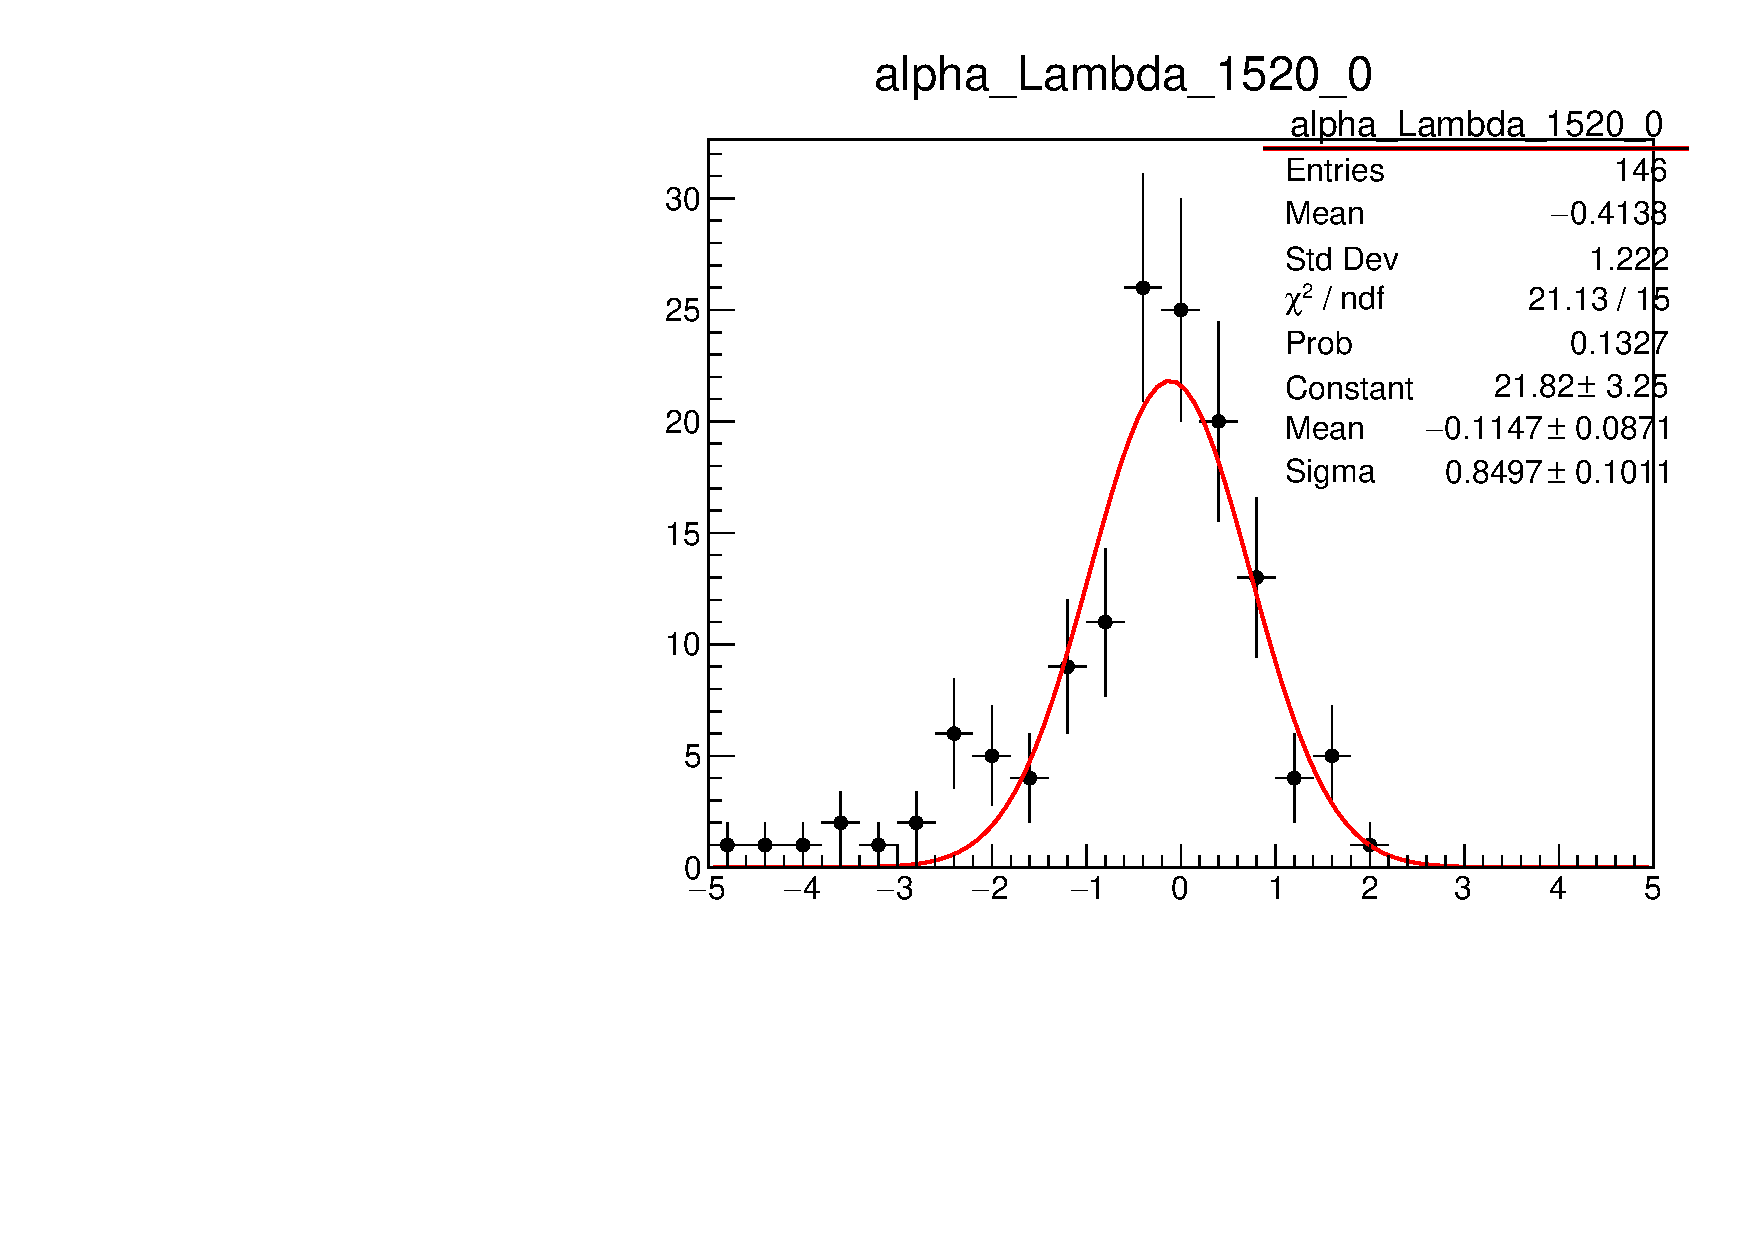
\includegraphics[width=0.24\textwidth]{figure/io_full_sim/alpha/pull_alpha_Lambda_1520_0.pdf}
    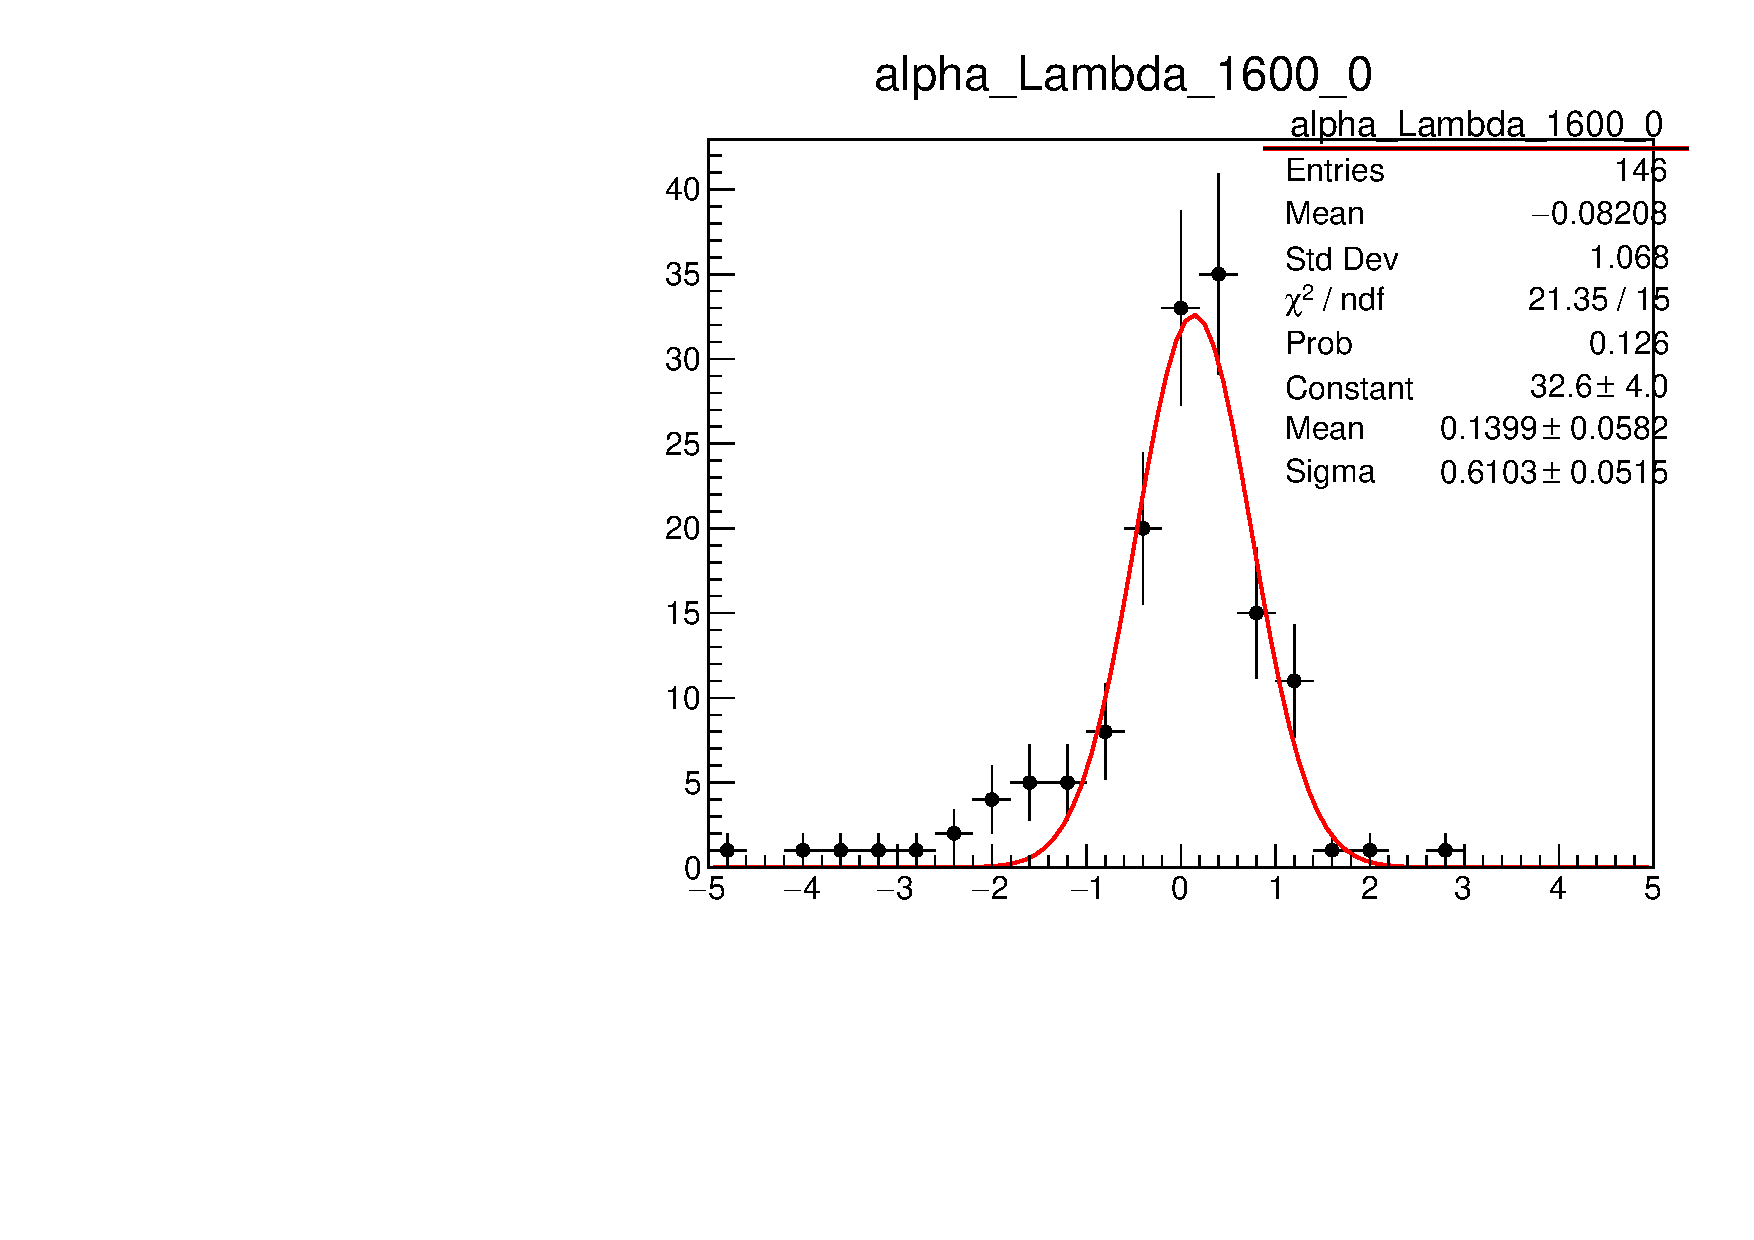
\includegraphics[width=0.24\textwidth]{figure/io_full_sim/alpha/pull_alpha_Lambda_1600_0.pdf}
    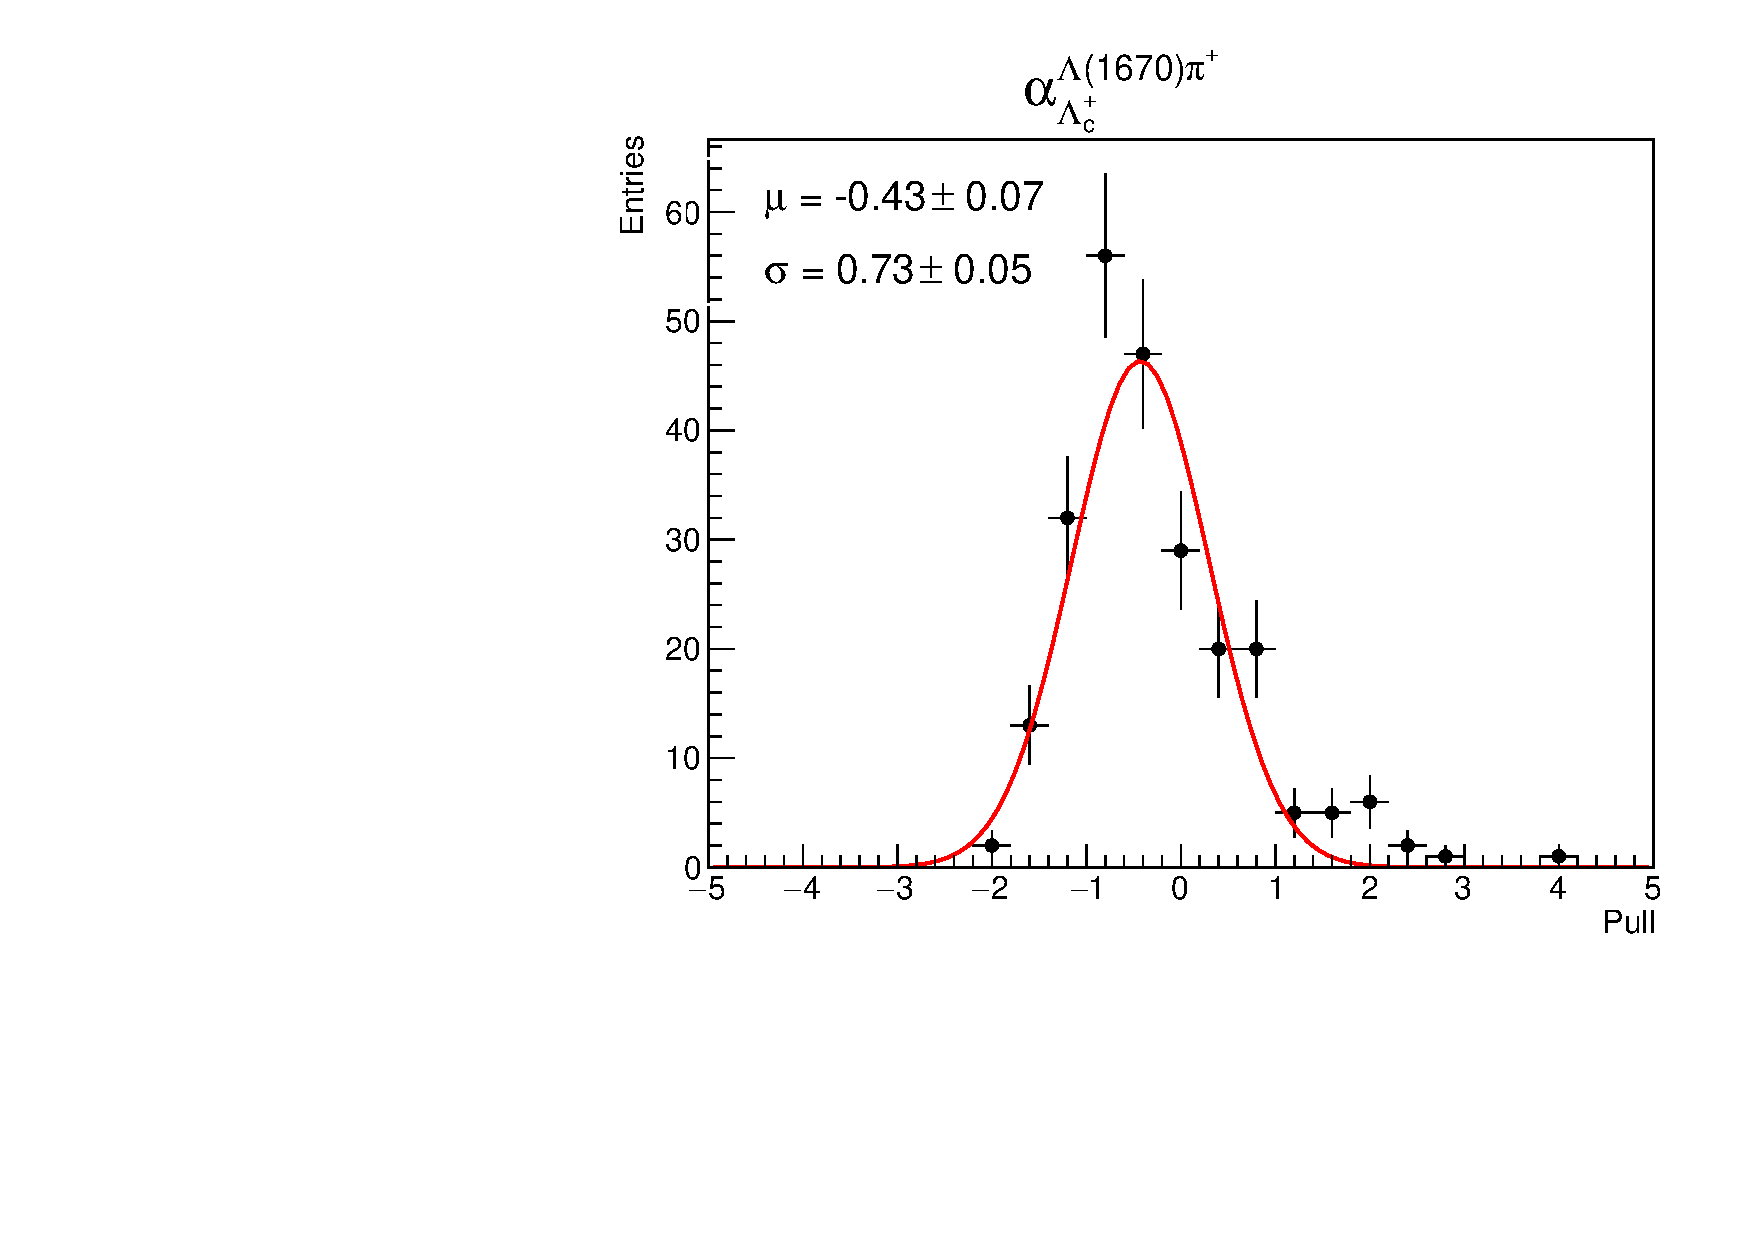
\includegraphics[width=0.24\textwidth]{figure/io_full_sim/alpha/pull_alpha_Lambda_1670_0.pdf}
    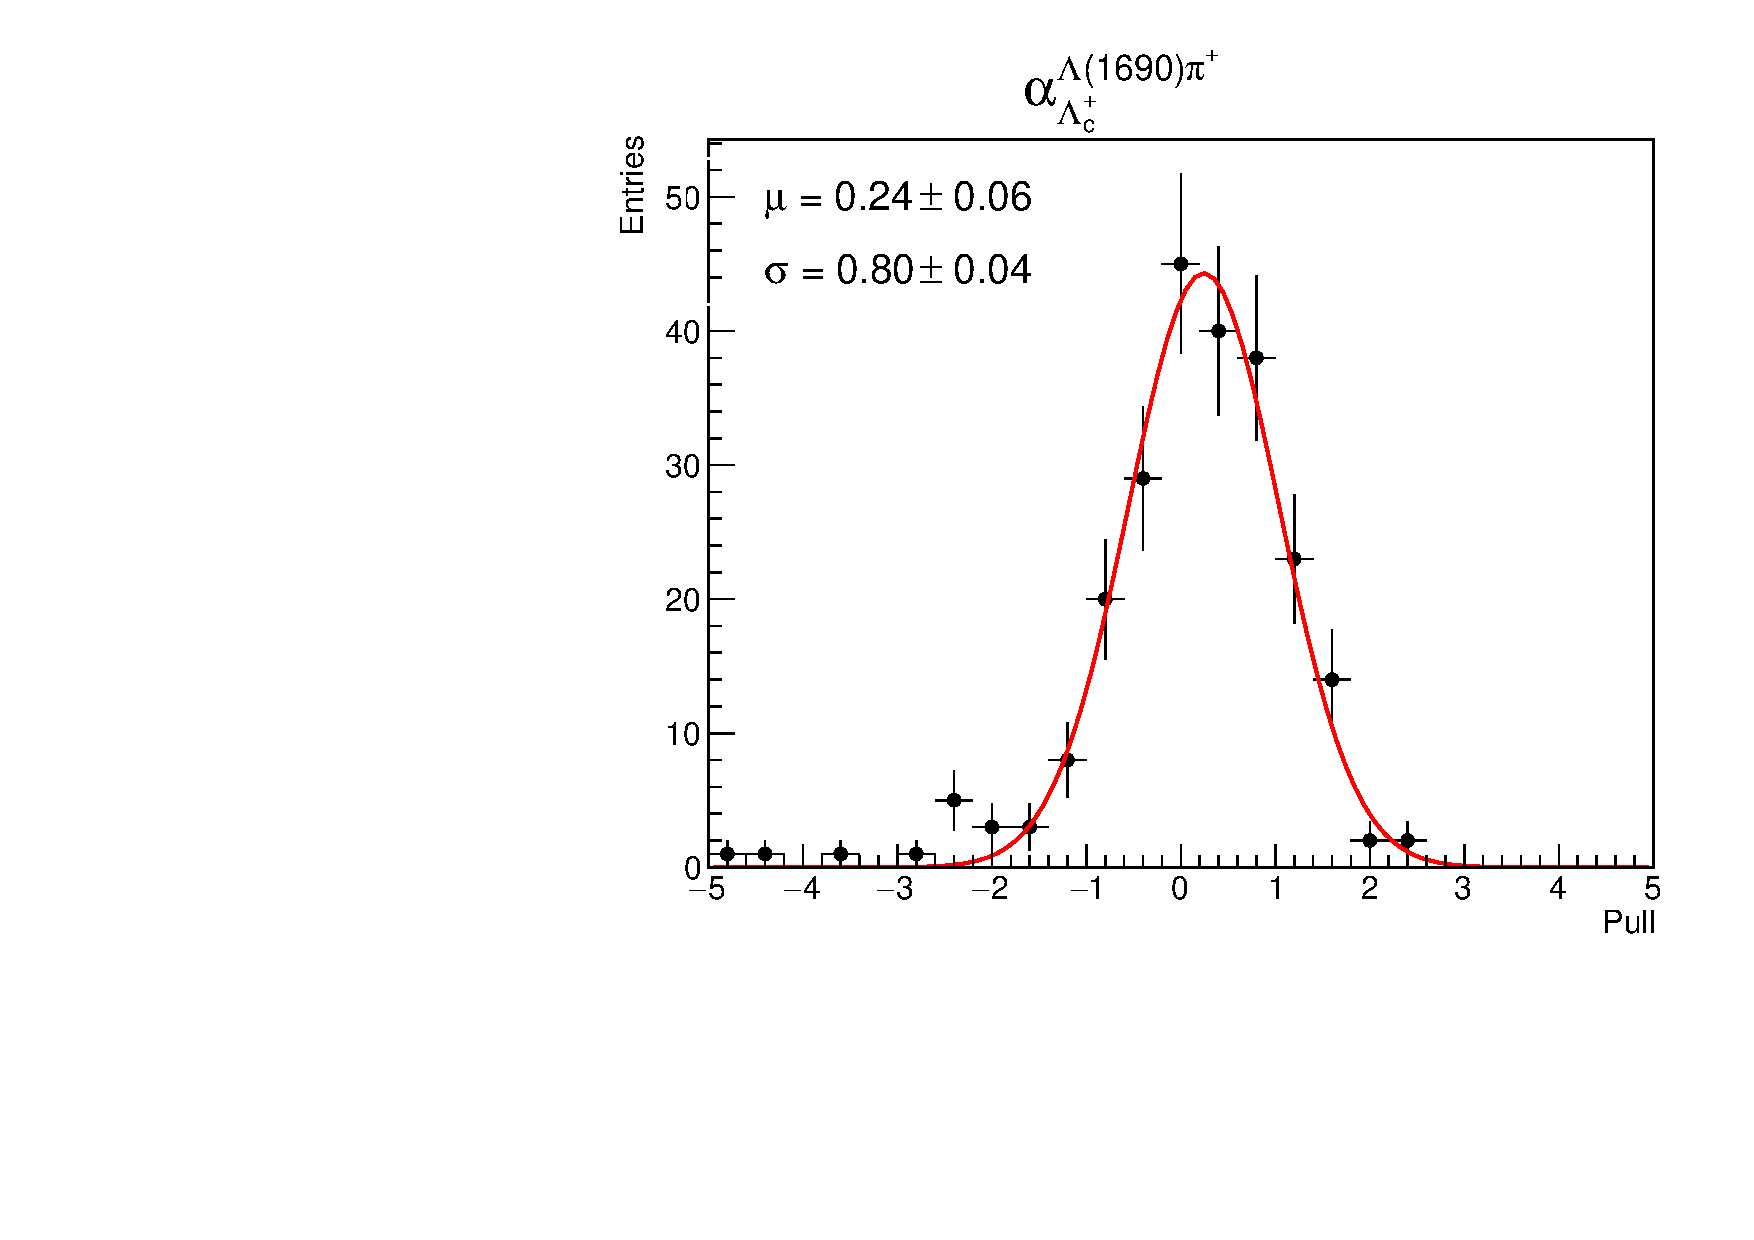
\includegraphics[width=0.24\textwidth]{figure/io_full_sim/alpha/pull_alpha_Lambda_1690_0.pdf}
    \includegraphics[width=0.24\textwidth]{figure/io_full_sim/alpha/pull_alpha_Lambda_2000_0.pdf}
    \includegraphics[width=0.24\textwidth]{figure/io_full_sim/alpha/pull_alpha_alpha_K_892_0.pdf}
    \includegraphics[width=0.24\textwidth]{figure/io_full_sim/alpha/pull_alpha_beta_K_892_0.pdf}
    \includegraphics[width=0.24\textwidth]{figure/io_full_sim/alpha/pull_alpha_gamma_K_892_0.pdf}
    \includegraphics[width=0.24\textwidth]{figure/io_full_sim/alpha/pull_alpha_lambda_K_892_0.pdf}
    \caption{Pull distributions for decay asymmetry parameters.}
\label{fig:io_wo_bkg_pull_asymmetry}
\end{figure}

\begin{figure}[h]\centering
    \includegraphics[width=0.24\textwidth]{figure/io_wo_bkg/gls/pull_gls_epem4600_Lmdc.aLmdc_g_ls_1r.pdf}
    \includegraphics[width=0.24\textwidth]{figure/io_wo_bkg/gls/pull_gls_epem4612_Lmdc.aLmdc_g_ls_1r.pdf}
    \includegraphics[width=0.24\textwidth]{figure/io_wo_bkg/gls/pull_gls_epem4626_Lmdc.aLmdc_g_ls_1r.pdf}
    \includegraphics[width=0.24\textwidth]{figure/io_wo_bkg/gls/pull_gls_epem4640_Lmdc.aLmdc_g_ls_1r.pdf}
    \includegraphics[width=0.24\textwidth]{figure/io_wo_bkg/gls/pull_gls_epem4660_Lmdc.aLmdc_g_ls_1r.pdf}
    \includegraphics[width=0.24\textwidth]{figure/io_wo_bkg/gls/pull_gls_epem4680_Lmdc.aLmdc_g_ls_1r.pdf}
    \includegraphics[width=0.24\textwidth]{figure/io_wo_bkg/gls/pull_gls_epem4700_Lmdc.aLmdc_g_ls_1r.pdf}
    \includegraphics[width=0.24\textwidth]{figure/io_wo_bkg/gls/pull_gls_epem4740_Lmdc.aLmdc_g_ls_1r.pdf}
    \includegraphics[width=0.24\textwidth]{figure/io_wo_bkg/gls/pull_gls_epem4750_Lmdc.aLmdc_g_ls_1r.pdf}
    \includegraphics[width=0.24\textwidth]{figure/io_wo_bkg/gls/pull_gls_epem4780_Lmdc.aLmdc_g_ls_1r.pdf}
    \includegraphics[width=0.24\textwidth]{figure/io_wo_bkg/gls/pull_gls_epem4840_Lmdc.aLmdc_g_ls_1r.pdf}
    \includegraphics[width=0.24\textwidth]{figure/io_wo_bkg/gls/pull_gls_epem4914_Lmdc.aLmdc_g_ls_1r.pdf}
    \includegraphics[width=0.24\textwidth]{figure/io_wo_bkg/gls/pull_gls_epem4946_Lmdc.aLmdc_g_ls_1r.pdf}
    \caption{Pull distributions for amplitude magnitudes of $e^+e^-\to\lcp\lcm$.}
\label{fig:io_wo_bkg_pull_magnitudes}
\end{figure}

\begin{figure}[h]\centering
    \includegraphics[width=0.24\textwidth]{figure/io_wo_bkg/gls/pull_gls_epem4600_Lmdc.aLmdc_g_ls_1i.pdf}
    \includegraphics[width=0.24\textwidth]{figure/io_wo_bkg/gls/pull_gls_epem4612_Lmdc.aLmdc_g_ls_1i.pdf}
    \includegraphics[width=0.24\textwidth]{figure/io_wo_bkg/gls/pull_gls_epem4626_Lmdc.aLmdc_g_ls_1i.pdf}
    \includegraphics[width=0.24\textwidth]{figure/io_wo_bkg/gls/pull_gls_epem4640_Lmdc.aLmdc_g_ls_1i.pdf}
    \includegraphics[width=0.24\textwidth]{figure/io_wo_bkg/gls/pull_gls_epem4660_Lmdc.aLmdc_g_ls_1i.pdf}
    \includegraphics[width=0.24\textwidth]{figure/io_wo_bkg/gls/pull_gls_epem4680_Lmdc.aLmdc_g_ls_1i.pdf}
    \includegraphics[width=0.24\textwidth]{figure/io_wo_bkg/gls/pull_gls_epem4700_Lmdc.aLmdc_g_ls_1i.pdf}
    \includegraphics[width=0.24\textwidth]{figure/io_wo_bkg/gls/pull_gls_epem4740_Lmdc.aLmdc_g_ls_1i.pdf}
    \includegraphics[width=0.24\textwidth]{figure/io_wo_bkg/gls/pull_gls_epem4750_Lmdc.aLmdc_g_ls_1i.pdf}
    \includegraphics[width=0.24\textwidth]{figure/io_wo_bkg/gls/pull_gls_epem4780_Lmdc.aLmdc_g_ls_1i.pdf}
    \includegraphics[width=0.24\textwidth]{figure/io_wo_bkg/gls/pull_gls_epem4840_Lmdc.aLmdc_g_ls_1i.pdf}
    \includegraphics[width=0.24\textwidth]{figure/io_wo_bkg/gls/pull_gls_epem4914_Lmdc.aLmdc_g_ls_1i.pdf}
    \includegraphics[width=0.24\textwidth]{figure/io_wo_bkg/gls/pull_gls_epem4946_Lmdc.aLmdc_g_ls_1i.pdf}
    \caption{Pull distributions for amplitude phases of $e^+e^-\to\lcp\lcm$.}
\label{fig:io_wo_bkg_pull_phase}
\end{figure}

\begin{table}[h]
    \caption{Fit results of pull distributions for $\alpha_0$ and $\Delta_0$ for each energy point.}
    \label{tab:fit_io_wo_bkg_pull_polarization}
    \resizebox{\textwidth}{!}{
        \begin{tabular}{cccccc}
            \hline\hline
        dataSet & $\mu_{\rm pull}$ & $\sigma_{\rm pull}$ & Nominal & Corrected & Difference \\\hline
        \multicolumn{6}{c}{$\alpha_0$} \\\hline
        4600 & 0.278 $\pm$ 0.059 & 0.914 $\pm$ 0.042 & -0.235 $\pm$ 0.037 & -0.225 $\pm$ 0.034 & 0.010\\
        4612 & -0.113 $\pm$ 0.063 & 0.971 $\pm$ 0.044 & -0.230 $\pm$ 0.093 & -0.240 $\pm$ 0.090 & 0.011\\
        4626 & 0.327 $\pm$ 0.067 & 1.033 $\pm$ 0.047 & -0.150 $\pm$ 0.044 & -0.135 $\pm$ 0.045 & 0.014\\
        4640 & 0.197 $\pm$ 0.064 & 0.997 $\pm$ 0.046 & -0.062 $\pm$ 0.046 & -0.053 $\pm$ 0.046 & 0.009\\
        4660 & 0.355 $\pm$ 0.068 & 1.046 $\pm$ 0.048 & 0.031 $\pm$ 0.052 & 0.050 $\pm$ 0.054 & 0.018\\
        4680 & 0.270 $\pm$ 0.067 & 1.043 $\pm$ 0.048 & 0.149 $\pm$ 0.033 & 0.158 $\pm$ 0.035 & 0.009\\
        4700 & -0.210 $\pm$ 0.060 & 0.922 $\pm$ 0.042 & 0.330 $\pm$ 0.070 & 0.315 $\pm$ 0.064 & 0.015\\
        4740 & -0.120 $\pm$ 0.067 & 1.044 $\pm$ 0.048 & 0.418 $\pm$ 0.159 & 0.399 $\pm$ 0.166 & 0.019\\
        4750 & -0.190 $\pm$ 0.060 & 0.926 $\pm$ 0.042 & 0.409 $\pm$ 0.103 & 0.389 $\pm$ 0.096 & 0.020\\
        4780 & -0.212 $\pm$ 0.060 & 0.934 $\pm$ 0.043 & 0.189 $\pm$ 0.078 & 0.173 $\pm$ 0.073 & 0.016\\
        4840 & -0.010 $\pm$ 0.060 & 0.935 $\pm$ 0.043 & 0.347 $\pm$ 0.107 & 0.346 $\pm$ 0.100 & 0.001\\
        4914 & -0.046 $\pm$ 0.085 & 1.276 $\pm$ 0.060 & 0.691 $\pm$ 0.196 & 0.682 $\pm$ 0.250 & 0.009\\
        4946 & -0.010 $\pm$ 0.057 & 0.868 $\pm$ 0.040 & 0.518 $\pm$ 0.225 & 0.515 $\pm$ 0.195 & 0.002\\\hline
        \multicolumn{6}{c}{$\sin\Delta_0$} \\\hline
        4600 & -0.080 $\pm$ 0.068 & 1.056 $\pm$ 0.048 & -0.178 $\pm$ 0.083 & -0.184 $\pm$ 0.088 & 0.007\\
        4612 & 0.165 $\pm$ 0.070 & 1.086 $\pm$ 0.050 & -0.393 $\pm$ 0.204 & -0.359 $\pm$ 0.222 & 0.034\\
        4626 & 0.045 $\pm$ 0.069 & 1.071 $\pm$ 0.049 & -0.228 $\pm$ 0.096 & -0.224 $\pm$ 0.102 & 0.004\\
        4640 & -0.153 $\pm$ 0.068 & 1.049 $\pm$ 0.048 & -0.433 $\pm$ 0.094 & -0.447 $\pm$ 0.098 & 0.014\\
        4660 & 0.280 $\pm$ 0.069 & 1.065 $\pm$ 0.049 & -0.483 $\pm$ 0.099 & -0.456 $\pm$ 0.105 & 0.028\\
        4680 & -0.255 $\pm$ 0.069 & 1.065 $\pm$ 0.049 & -0.470 $\pm$ 0.063 & -0.486 $\pm$ 0.067 & 0.016\\
        4700 & 0.152 $\pm$ 0.068 & 1.058 $\pm$ 0.048 & -0.568 $\pm$ 0.134 & -0.548 $\pm$ 0.141 & 0.020\\
        4740 & -0.002 $\pm$ 0.062 & 0.956 $\pm$ 0.044 & 0.231 $\pm$ 0.287 & 0.230 $\pm$ 0.274 & 0.000\\
        4750 & 0.252 $\pm$ 0.065 & 1.009 $\pm$ 0.046 & -0.370 $\pm$ 0.199 & -0.320 $\pm$ 0.201 & 0.050\\
        4780 & 0.232 $\pm$ 0.067 & 1.032 $\pm$ 0.047 & -0.395 $\pm$ 0.146 & -0.361 $\pm$ 0.150 & 0.034\\
        4840 & -0.126 $\pm$ 0.062 & 0.950 $\pm$ 0.044 & -0.502 $\pm$ 0.215 & -0.529 $\pm$ 0.205 & 0.027\\
        4914 & -0.147 $\pm$ 0.060 & 0.827 $\pm$ 0.042 & 0.389 $\pm$ 0.430 & 0.325 $\pm$ 0.356 & 0.063\\
        4946 & -0.019 $\pm$ 0.058 & 0.834 $\pm$ 0.041 & -0.295 $\pm$ 0.420 & -0.303 $\pm$ 0.350 & 0.008\\
        \hline\hline
        \end{tabular}
        }
\end{table}

\begin{table}[h]
    \caption{Fit results of pull distributions for FF of each resonance.}
    \label{tab:fit_io_wo_bkg_pull_ff}
    \resizebox{\textwidth}{!}{
        \begin{tabular}{cccccc}
            \hline\hline
            Resonance & $\mu_{\text{pull}}$ & $\sigma_{\text{pull}}$ & Nominal FF (\%) & Corrected FF (\%) & Difference (\%)\\\hline
            $\Delta(1232)^{++}$ & 0.11$\pm$0.07 & 0.94$\pm$0.05 & 27.31$\pm$1.04 & 27.20$\pm$0.98 & 0.11\\
            $\Delta(1600)^{++}$ & 0.25$\pm$0.06 & 0.95$\pm$0.06 & 7.44$\pm$1.73 & 7.00$\pm$1.64 & 0.44\\
            $\Delta(1600)^{++}$ & 0.43$\pm$0.07 & 0.97$\pm$0.05 & 4.77$\pm$1.73 & 4.02$\pm$1.67 & 0.75\\
            $\Delta(1700)^{++}$ & 0.51$\pm$0.06 & 0.87$\pm$0.05 & 11.98$\pm$1.37 & 11.29$\pm$1.18 & 0.69\\
            $K_{0}^{*}(1430)$ & 0.05$\pm$0.07 & 0.95$\pm$0.07 & 14.63$\pm$2.83 & 14.50$\pm$2.69 & 0.13\\
            $K_{0}^{*}(700)$ & 0.30$\pm$0.06 & 0.83$\pm$0.05 & 2.60$\pm$0.59 & 2.43$\pm$0.49 & 0.18\\
            $K^{*}(892)$ & -1.06$\pm$0.06 & 0.88$\pm$0.05 & 23.70$\pm$1.31 & 25.09$\pm$1.15 & -1.39\\
            $\Lambda(1405)$ & -0.03$\pm$0.07 & 1.01$\pm$0.06 & 4.45$\pm$1.16 & 4.48$\pm$1.17 & -0.03\\
            $\Lambda(1520)$ & -0.53$\pm$0.07 & 1.01$\pm$0.05 & 1.27$\pm$0.18 & 1.36$\pm$0.18 & -0.10\\
            $\Lambda(1600)$ & -0.05$\pm$0.06 & 0.91$\pm$0.05 & 4.77$\pm$1.06 & 4.82$\pm$0.97 & -0.05\\
            $\Lambda(1670)$ & 0.29$\pm$0.07 & 0.98$\pm$0.06 & 1.69$\pm$0.26 & 1.61$\pm$0.25 & 0.08\\
            $\Lambda(1690)$ & -0.30$\pm$0.09 & 1.27$\pm$0.07 & 0.91$\pm$0.24 & 0.98$\pm$0.30 & -0.07\\
            $\Lambda(2000)$ & 0.05$\pm$0.08 & 1.12$\pm$0.08 & 6.24$\pm$0.54 & 6.21$\pm$0.60 & 0.03\\\hline
            Sum& & & 111.76$\pm$4.68 & 111.00$\pm$4.41 & \\
        \hline\hline
        \end{tabular}
        }
\end{table}


\begin{table}[h]
    \caption{Fit results of pull distributions for decay asymmetry parameters.}
    \label{tab:fit_io_wo_bkg_pull_alpha}
    \resizebox{\textwidth}{!}{
        \begin{tabular}{cccccc}
            \hline\hline
            Parameters & $\mu_{\text{pull}}$ & $\sigma_{\text{pull}}$ & Nominal & Corrected & Difference\\\hline
            $\alpha_{\Lambda_c^+}^{\pi^{+}\Lambda(1520)}$ & 0.328$\pm$0.064 & 0.957$\pm$0.057 & -0.373$\pm$0.275 & -0.283$\pm$0.263 & 0.090\\
            $\alpha_{\Lambda_c^+}^{\pi^{+}\Lambda(1690)}$ & 0.243$\pm$0.055 & 0.799$\pm$0.042 & -0.875$\pm$0.121 & -0.846$\pm$0.097 & 0.029\\
            $\alpha_{\Lambda_c^+}^{K^{-}\Delta(1232)^{++}}$ & 0.063$\pm$0.073 & 1.042$\pm$0.070 & -0.707$\pm$0.097 & -0.701$\pm$0.101 & 0.006\\
            $\alpha_{\Lambda_c^+}^{K^{-}\Delta(1600)^{++}}$ & 0.246$\pm$0.075 & 1.119$\pm$0.054 & -0.113$\pm$0.216 & -0.059$\pm$0.242 & 0.053\\
            $\alpha_{\Lambda_c^+}^{K^{-}\Delta(1700)^{++}}$ & -0.593$\pm$0.068 & 1.003$\pm$0.071 & -0.141$\pm$0.069 & -0.181$\pm$0.069 & 0.041\\
            $\alpha_{\Lambda_c^+}^{\pi^{+}\Lambda(1405)}$ & 0.006$\pm$0.076 & 0.948$\pm$0.073 & -0.100$\pm$0.424 & -0.097$\pm$0.402 & 0.002\\
            $\alpha_{\Lambda_c^+}^{\pi^{+}\Lambda(1600)}$ & -0.190$\pm$0.075 & 0.991$\pm$0.060 & -0.749$\pm$0.144 & -0.777$\pm$0.142 & 0.027\\
            $\alpha_{\Lambda_c^+}^{\pi^{+}\Lambda(1670)}$ & -0.428$\pm$0.067 & 0.725$\pm$0.054 & 0.943$\pm$0.095 & 0.902$\pm$0.069 & 0.041\\
            $\alpha_{\Lambda_c^+}^{\pi^{+}\Lambda(2000)}$ & 0.157$\pm$0.072 & 1.031$\pm$0.064 & -0.824$\pm$0.089 & -0.810$\pm$0.092 & 0.014\\
            $\alpha_{\Lambda_c^+}^{K^{-}\Delta(1620)^{++}}$ & 0.141$\pm$0.075 & 1.095$\pm$0.062 & 0.222$\pm$0.259 & 0.259$\pm$0.284 & 0.037\\
            $\alpha_{\Lambda_c^+}^{p\overline{K}^*_0(700)}$ & 0.477$\pm$0.072 & 1.037$\pm$0.062 & 0.040$\pm$0.321 & 0.194$\pm$0.333 & 0.153\\
            $\alpha_{\Lambda_c^+}^{p\overline{K}^*_0(1430)}$ & 0.237$\pm$0.082 & 1.131$\pm$0.062 & -0.225$\pm$0.066 & -0.209$\pm$0.075 & 0.016\\
            $\alpha_{\Lambda_c^+}^{p\overline{K}^*(892)}$ & 0.272$\pm$0.069 & 0.890$\pm$0.082 & -0.791$\pm$0.097 & -0.765$\pm$0.086 & 0.026\\
            $\beta_{\Lambda_c^+}^{p\overline{K}^*(892)}$ & -0.433$\pm$0.087 & 1.149$\pm$0.073 & -0.599$\pm$0.239 & -0.702$\pm$0.275 & 0.103\\
            $\gamma_{\Lambda_c^+}^{p\overline{K}^*(892)}$ & 0.138$\pm$0.077 & 1.089$\pm$0.073 & 1.478$\pm$0.168 & 1.501$\pm$0.183 & 0.023\\
            $\Lambda_{\Lambda_c^+}^{p\overline{K}^*(892)}$ & -0.186$\pm$0.075 & 1.038$\pm$0.061 & -0.713$\pm$0.102 & -0.732$\pm$0.106 & 0.019\\
        \hline\hline
        \end{tabular}
        }
\end{table}

\begin{table}[h]
    \caption{Fit results of pull distributions for amplitude magnitudes and phases of $e^+e^-\to\lcp\lcm$.}
    \label{tab:fit_io_wo_bkg_pull_gls}
    \resizebox{\textwidth}{!}{
        \begin{tabular}{cccccc}
        \hline\hline
        Parameters & $\mu_{\text{pull}}$ & $\sigma_{\text{pull}}$ & Nominal & Corrected & Difference (\%)\\\hline
        epem4600$->$Lmdc.aLmdc$\_$g$\_$ls$\_$1i & -0.02$\pm$0.07 & 0.96$\pm$0.06 & -0.39$\pm$0.17 & -0.39$\pm$0.16 & -0.00 \\
        epem4600$->$Lmdc.aLmdc$\_$g$\_$ls$\_$1r & -0.40$\pm$0.06 & 0.90$\pm$0.05 & 4.08$\pm$0.42 & 4.25$\pm$0.38 & -0.17 \\
        epem4612$->$Lmdc.aLmdc$\_$g$\_$ls$\_$1i & 0.09$\pm$0.10 & 0.95$\pm$0.07 & -2.04$\pm$0.33 & -2.07$\pm$0.32 & 0.03 \\
        epem4612$->$Lmdc.aLmdc$\_$g$\_$ls$\_$1r & -0.09$\pm$0.07 & 0.91$\pm$0.06 & 0.23$\pm$0.10 & 0.24$\pm$0.09 & -0.01 \\
        epem4626$->$Lmdc.aLmdc$\_$g$\_$ls$\_$1i & 0.11$\pm$0.08 & 1.10$\pm$0.06 & -0.42$\pm$0.16 & -0.44$\pm$0.18 & 0.02 \\
        epem4626$->$Lmdc.aLmdc$\_$g$\_$ls$\_$1r & -0.33$\pm$0.08 & 1.11$\pm$0.06 & 3.35$\pm$0.34 & 3.46$\pm$0.38 & -0.11 \\
        epem4640$->$Lmdc.aLmdc$\_$g$\_$ls$\_$1i & 0.30$\pm$0.07 & 0.96$\pm$0.07 & -1.64$\pm$0.12 & -1.67$\pm$0.11 & 0.04 \\
        epem4640$->$Lmdc.aLmdc$\_$g$\_$ls$\_$1r & 0.11$\pm$0.07 & 1.07$\pm$0.06 & 0.22$\pm$0.05 & 0.21$\pm$0.05 & 0.01 \\
        epem4660$->$Lmdc.aLmdc$\_$g$\_$ls$\_$1i & 0.39$\pm$0.06 & 0.96$\pm$0.05 & -0.63$\pm$0.11 & -0.68$\pm$0.11 & 0.04 \\
        epem4660$->$Lmdc.aLmdc$\_$g$\_$ls$\_$1r & -0.06$\pm$0.07 & 1.03$\pm$0.05 & 2.17$\pm$0.22 & 2.18$\pm$0.23 & -0.01 \\
        epem4680$->$Lmdc.aLmdc$\_$g$\_$ls$\_$1i & 0.18$\pm$0.07 & 1.01$\pm$0.05 & -1.18$\pm$0.07 & -1.19$\pm$0.07 & 0.01 \\
        epem4680$->$Lmdc.aLmdc$\_$g$\_$ls$\_$1r & 0.25$\pm$0.07 & 1.01$\pm$0.06 & 0.24$\pm$0.03 & 0.23$\pm$0.03 & 0.01 \\
        epem4700$->$Lmdc.aLmdc$\_$g$\_$ls$\_$1i & -0.03$\pm$0.07 & 0.89$\pm$0.05 & -0.93$\pm$0.11 & -0.92$\pm$0.10 & -0.00 \\
        epem4700$->$Lmdc.aLmdc$\_$g$\_$ls$\_$1r & -0.18$\pm$0.07 & 1.02$\pm$0.07 & 0.31$\pm$0.07 & 0.33$\pm$0.07 & -0.01 \\
        epem4740$->$Lmdc.aLmdc$\_$g$\_$ls$\_$1i & 0.06$\pm$0.07 & 0.97$\pm$0.05 & 0.20$\pm$0.24 & 0.18$\pm$0.24 & 0.01 \\
        epem4740$->$Lmdc.aLmdc$\_$g$\_$ls$\_$1r & -0.13$\pm$0.06 & 0.88$\pm$0.05 & 1.67$\pm$0.29 & 1.70$\pm$0.26 & -0.04 \\
        epem4750$->$Lmdc.aLmdc$\_$g$\_$ls$\_$1i & 0.22$\pm$0.07 & 0.96$\pm$0.04 & -0.32$\pm$0.17 & -0.35$\pm$0.16 & 0.04 \\
        epem4750$->$Lmdc.aLmdc$\_$g$\_$ls$\_$1r & 0.13$\pm$0.06 & 0.88$\pm$0.04 & 1.62$\pm$0.20 & 1.59$\pm$0.18 & 0.03 \\
        epem4780$->$Lmdc.aLmdc$\_$g$\_$ls$\_$1i & 0.02$\pm$0.07 & 0.93$\pm$0.05 & -0.44$\pm$0.15 & -0.44$\pm$0.14 & 0.00 \\
        epem4780$->$Lmdc.aLmdc$\_$g$\_$ls$\_$1r & 0.18$\pm$0.06 & 0.90$\pm$0.05 & 1.97$\pm$0.23 & 1.93$\pm$0.21 & 0.04 \\
        epem4840$->$Lmdc.aLmdc$\_$g$\_$ls$\_$1i & -0.13$\pm$0.06 & 0.88$\pm$0.04 & -0.85$\pm$0.21 & -0.83$\pm$0.19 & -0.03 \\
        epem4840$->$Lmdc.aLmdc$\_$g$\_$ls$\_$1r & 0.19$\pm$0.06 & 0.65$\pm$0.04 & 0.28$\pm$0.10 & 0.27$\pm$0.07 & 0.02 \\
        epem4914$->$Lmdc.aLmdc$\_$g$\_$ls$\_$1i & 0.10$\pm$0.06 & 0.88$\pm$0.05 & 0.22$\pm$0.24 & 0.20$\pm$0.21 & 0.02 \\
        epem4914$->$Lmdc.aLmdc$\_$g$\_$ls$\_$1r & -0.13$\pm$0.06 & 0.88$\pm$0.06 & 1.23$\pm$0.30 & 1.27$\pm$0.26 & -0.04 \\
        epem4946$->$Lmdc.aLmdc$\_$g$\_$ls$\_$1i & -0.22$\pm$0.08 & 1.12$\pm$0.07 & -0.41$\pm$0.51 & -0.30$\pm$0.57 & -0.11 \\
        epem4946$->$Lmdc.aLmdc$\_$g$\_$ls$\_$1r & 0.25$\pm$0.04 & 0.54$\pm$0.03 & 0.27$\pm$0.14 & 0.24$\pm$0.08 & 0.04 \\
        \hline\hline
        \end{tabular}
        }
\end{table}